%
%
% UCSD Doctoral Dissertation Template
% -----------------------------------
% http://ucsd-thesis.googlecode.com
%
%
% ----------------------------------------------------------------------
% WARNING: 
%
%   This template has not endorced by OGS or any other official entity.
%   The official formatting guide can be obtained from OGS.
%   It can be found on the web here:
%   http://ogs.ucsd.edu/AcademicAffairs/Documents/Dissertations_Theses_Formatting_Manual.pdf
%
%   No guaranty is made that this LaTeX class conforms to the official UCSD guidelines.
%   Make sure that you check the final document against the Formatting Manual.
%  
%   That being said, this class has been routinely used for successful 
%   publication of doctoral theses.  
%
%   The ucsd.cls class files are only valid for doctoral dissertations.
%
%
% ----------------------------------------------------------------------
% GETTING STARTED:
%
%   Lots of information can be found on the project wiki:
%   http://code.google.com/p/ucsd-thesis/wiki/GettingStarted
%
%
%   To make a pdf from this template use the command:
%     pdflatex template
%
%
%   To get started please read the comments in this template file 
%   and make changes as appropriate.
%
%   If you successfully submit a thesis with this package please let us
%   know.
%
%
% ----------------------------------------------------------------------
% KNOWN ISSUES:
%
%   Currently only the 12pt size conforms to the UCSD requirements.
%   The 10pt and 11pt options make the footnote fonts too small.
%
%
% ----------------------------------------------------------------------
% HELP/CONTACT:
%
%   If you need help try the ucsd-thesis google group:
%   http://groups.google.com/group/ucsd-thesis
%
%
% ----------------------------------------------------------------------
% BUGS:
%
%   Please report all bugs at:
%   http://code.google.com/p/ucsd-thesis/issues/list
%
%
% ----------------------------------------------------------------------
% More control of the formatting of your thesis can be achieved through
% modifications of the included LaTeX class files:
%
%   * ucsd.cls    -- Class file
%   * uct10.clo   -- Configuration files for font sizes 10pt, 11pt, 12pt
%     uct11.clo                            
%     uct12.clo
%
% ----------------------------------------------------------------------



% Setup the documentclass 
% default options: 12pt, oneside, final
%
% fonts: 10pt, 11pt, 12pt -- are valid for UCSD dissertations.
% sides: oneside, twoside -- note that two-sided theses are not accepted 
%                            by OGS.
% mode: draft, final      -- draft mode switches to single spacing, 
%                            removes hyperlinks, and places a black box
%                            at every overfull hbox (check these before
%                            submission).
% chapterheads            -- Include this if you want your chapters to read:
%                              Chapter 1
%                              Title of Chapter
%
%                            instead of
%                              1 Title of Chapter
\documentclass[12pt,chapterheads]{ucsd}



% Include all packages you need here.  
% Some standard options are suggested below.
%
% See the project wiki for information on how to use 
% these packages. Other useful packages are also listed there.
%
%   http://code.google.com/p/ucsd-thesis/wiki/GettingStarted



%% AMS PACKAGES - Chances are you will want some or all 
%    of these if writing a dissertation that includes equations.
%  \usepackage{amsmath, amscd, amssymb, amsthm}

%% GRAPHICX - This is the standard package for 
%    including graphics for latex/pdflatex.
\usepackage{scrextend}
\usepackage{pslatex}
\usepackage{graphicx}

%% CAPTION
% This overrides some of the ugliness in ucsd.cls and
% allows the text to be double-spaced while letting figures,
% tables, and footnotes to be single-spaced--all OGS requirements.
% NOTE: Must appear after graphics and ams math
\makeatletter
\gdef\@ptsize{2}% 12pt documents
\let\@currsize\normalsize
\makeatother
\usepackage{setspace}
\doublespace
\usepackage[font=small, width=0.9\textwidth]{caption}

%% SUBFIG - Use this to place multiple images in a
%    single figure.  Subfig will handle placement and
%    proper captioning (e.g. Figure 1.2(a))
% \usepackage{subfig}

%% TIMES FONT - replacements for Computer Modern
%%   This package will replace the default font with a
%%   Times-Roman font with math support.
% \usepackage[T1]{fontenc}
% \usepackage{mathptmx}

%% INDEX
%   Uncomment the following two lines to create an index: 
\usepackage{makeidx}
\makeindex
%   You will need to uncomment the \printindex line near the
%   bibliography to display the index.  Use the command
% \index{keyword} 
%   within the text to create an entry in the index for keyword.
%   To compile a LaTeX document with an index the 'makeindex'
%   command will need to be run.  See the wiki for more details.

%% HYPERLINKS
%   To create a PDF with hyperlinks, you need to include the hyperref package.
%   THIS HAS TO BE THE LAST PACKAGE INCLUDED!
%   Note that the options plainpages=false and pdfpagelabels exist
%   to fix indexing associated with having both (ii) and (2) as pages.
%   Also, all links must be black according to OGS.
%   See: http://www.tex.ac.uk/cgi-bin/texfaq2html?label=hyperdupdest
%   Note: This may not work correctly with all DVI viewers (i.e. Yap breaks).
%   NOTE: hyperref will NOT work in draft mode, as noted above.
% \usepackage[colorlinks=true, pdfstartview=FitV, 
%             linkcolor=black, citecolor=black, 
%             urlcolor=black, plainpages=false,
%             pdfpagelabels]{hyperref}
% \hypersetup{ pdfauthor = {Your Name Here}, 
%              pdftitle = {The Title of The Dissertation}, 
%              pdfkeywords = {Keywords for Searching}, 
%              pdfcreator = {pdfLaTeX with hyperref package}, 
%              pdfproducer = {pdfLaTeX} }
% \urlstyle{same}
% \usepackage{bookmark}


%% CITATIONS
% Sets citation format
% and fixes up citations madness
\usepackage{microtype}  % avoids citations that hang into the margin


%% FOOTNOTE-MAGIC
% Enables footnotes in tables, re-referencing the same footnote multiple times.
\usepackage{footnote}
\makesavenoteenv{tabular}
\makesavenoteenv{table}


%% TABLE FORMATTING MADNESS
% Enable all sorts of fun table tricks
\usepackage{rotating}  % Enables the sideways environment (NCPW)
\usepackage{array}  % Enables "m" tabular environment http://ctan.org/pkg/array
\usepackage{booktabs}  % Enables \toprule  http://ctan.org/pkg/array



\begin{document}

%% FRONT MATTER
%
%  All of the front matter.
%  This includes the title, degree, dedication, vita, abstract, etc..
%  Modify the file template_frontmatter.tex to change these pages.
%
%
% UCSD Doctoral Dissertation Template
% -----------------------------------
% http://ucsd-thesis.googlecode.com
%
%


%% REQUIRED FIELDS -- Replace with the values appropriate to you

% No symbols, formulas, superscripts, or Greek letters are allowed
% in your title.
\title{Methods for Integrative Analysis of RNA Binding Proteins}

\author{Gabriel Asbury Pratt}
\degreeyear{2018}

% Master's Degree theses will NOT be formatted properly with this file.
\degreetitle{Doctor of Philosophy}

\field{Bioinformatics and Systems Biology}
%\specialization{Anthropogeny}  % If you have a specialization, add it here

\chair{Professor Gene Yeo}
% Uncomment the next line iff you have a Co-Chair
\cochair{Professor Sheng Zhong}
%
% Or, uncomment the next line iff you have two equal Co-Chairs.
%\cochairs{Professor Chair Masterish}{Professor Chair Masterish}

%  The rest of the committee members  must be alphabetized by last name.
\othermembers{
Professor Jens Lykke-Andersen\\
Professor Bing Ren\\
Professor Joseph Simpson\\
}
\numberofmembers{5} % |chair| + |cochair| + |othermembers|


%% START THE FRONTMATTER
%
\begin{frontmatter}

%% TITLE PAGES
%
%  This command generates the title, copyright, and signature pages.
%
\makefrontmatter

%% DEDICATION
%
%  You have three choices here:
%    1. Use the ``dedication'' environment.
%       Put in the text you want, and everything will be formated for
%       you. You'll get a perfectly respectable dedication page.
%
%
%    2. Use the ``mydedication'' environment.  If you don't like the
%       formatting of option 1, use this environment and format things
%       however you wish.
%
%    3. If you don't want a dedication, it's not required.
%
%
\begin{dedication}
  To my parents who taught me to be curious, my mentors who showed me the cool things to be curious about, my friends who kept me balanced through out all of this.  
\end{dedication}


% \begin{mydedication} % You are responsible for formatting here.
%   \vspace{1in}
%   \begin{flushleft}
% 	To me.
%   \end{flushleft}
%
%   \vspace{2in}
%   \begin{center}
% 	And you.
%   \end{center}
%
%   \vspace{2in}
%   \begin{flushright}
% 	Which equals us.
%   \end{flushright}
% \end{mydedication}



%% EPIGRAPH
%
%  The same choices that applied to the dedication apply here.
%
\begin{epigraph} % The style file will position the text for you.
  \emph{Progress isn't made by early risers.
                 It's made by lazy men trying to find easier ways to do something}\\
  ---Robert Heinlein
\end{epigraph}

% \begin{myepigraph} % You position the text yourself.
%   \vfil
%   \begin{center}
%     {\bf Think! It ain't illegal yet.}
%
% 	\emph{---George Clinton}
%   \end{center}
% \end{myepigraph}


%% SETUP THE TABLE OF CONTENTS
%
\tableofcontents
\listoffigures  % Comment if you don't have any figures
%\listoftables   % Comment if you don't have any tables



%% ACKNOWLEDGEMENTS
%
%  While technically optional, you probably have someone to thank.
%  Also, a paragraph acknowledging all coauthors and publishers (if
%  you have any) is required in the acknowledgements page and as the
%  last paragraph of text at the end of each respective chapter. See
%  the OGS Formatting Manual for more information.
%
\begin{acknowledgements}
To all my co-authors and lab mates I    couldn't have done this without you.    Specifically I want to call out Mike Lovci, who taught me how to analyze CLIP-seq data.  I’ve leaned on your tools more than you know.  Katannya Kapeli who was the first person to drag me through a full biological story.  Finally I wouldn’t have finished my PhD with out Eric Van Nostrand, who taught me everything else, but most importantly taught me how to walk carefully through analyses instead of just running ahead. I wouldn’t be half the researcher I am without out.

I also want acknowledge the people who put me on this path. My high school Genetics teacher Penny Pagels, who first introduced me to the field.  Chuck Murry who took a chance on a first year undergrad who wanted to work in a lab. My two main undergraduate mentors, Jonathan Golob, who exposed me to everything bioinformatics could be and Sharron Paige, who let me help on the coolest projects.

A short acknowledgement, cannot properly recognize everyone who has helped me along the way, or encompass what I’ve learned from everyone.  I am eternally grateful for all the time and energy you all have invested, and hope to pay it back some day.

\end{acknowledgements}


%% VITA
%
%  A brief vita is required in a doctoral thesis. See the OGS
%  Formatting Manual for more information.
%
\begin{vitapage}
\begin{vita}
  \item[2011] B.~S. in Computer Science, University of Washington, Seattle
  \item[2018] Ph.~D. in Bioinformatics and Systems Biology, University of California, San Diego
\end{vita}
\begin{publications}

        \item Gabriel A. Pratt, Eric L. Van Nostrand, Brian A. Yee, Alain Domissy, Steven M. Blue, Chelsea Gelboin-Burkhart, Thai B. Nguyen, Ines Rabano, Ruth Wang, Balaji Sundararaman, Keri Garcia, Rebecca Stanton, Gene W. Yeo. ``Guidelines and Best Practices for enhanced CLIP experiments and analysis''. \emph{In Submission}, 2017
        \item Eric L Van Nostrand§, Peter Freese§, Gabriel A Pratt§, Xiaofeng Wang§, Xintao Wei§, Rui Xiao§, Steven M Blue, Daniel Dominguez, Neal A.L. Cody, Sara Olson, Balaji Sundararaman, Lijun Zhan, Cassandra Bazile, Louis Philip Benoit Bouvrette, Jiayu Chen, Michael O Duff, Keri E. Garcia, Chelsea Gelboin-Burkhart, Abigail Hochman, Nicole J Lambert, Hairi Li, Thai B Nguyen, Tsultrim Palden, Ines Rabano, Shashank Sathe, Rebecca Stanton, Julie Bergalet, Bing Zhou, Amanda Su, Ruth Wang, Brian A. Yee, Ashley L Louie, Stefan Aigner, Xiang-dong Fu, Eric Lecuyer, Christopher B. Burge, Brenton R. Graveley, Gene W. Yeo. ``A Large-Scale Binding and Functional Map of Human RNA Binding Proteins'' \emph{In Submission}, 2017
        \item Eric L Van Nostrand, Chelsea Gelboin-Burkhart, Ruth Wang, Gabriel A Pratt, Steven M Blue, Gene W Yeo. ``CRISPR/Cas9-mediated integration enables TAG-eCLIP of endogenously tagged RNA binding proteins''. \emph{Methods}, 2016
      \item Fernando J Martinez, Gabriel A Pratt, Eric L Van Nostrand, Ranjan Batra, Stephanie C Huelga, Katannya Kapeli, Peter Freese, Seung J Chun, Karen Ling, Chelsea Gelboin-Burkhart, Layla Fijany, Harrison C Wang, Julia K Nussbacher, Sara M Broski, Hong Joo Kim, Rea Lardelli, Balaji Sundararaman, John P Donohue, Ashkan Javaherian, Jens Lykke-Andersen, Steven Finkbeiner, C Frank Bennett, Manuel Ares, Christopher B Burge, J Paul Taylor, Frank Rigo, Gene W Yeo. ``Protein-RNA Networks Regulated by Normal and ALS-Associated Mutant HNRNPA2B1 in the Nervous System.'' \emph{Neuron}, 2016
      \item Kristopher W Brannan, Wenhao Jin, Stephanie C Huelga, Charles AS Banks, Joshua M Gilmore, Laurence Florens, Michael P Washburn, Eric L Van Nostrand, Gabriel A Pratt, Marie K Schwinn, Danette L Daniels, Gene W Yeo. ``SONAR Discovers RNA-Binding Proteins from Analysis of Large-Scale Protein-Protein Interactomes.'' \emph{Molecular Cell}, 2016
      \item Katannya Kapeli§, Gabriel A. Pratt§, Anthony Q. Vu, Kasey R. Hutt, Fernando J. Martinez, Balaji Sundararaman, Ranjan Batra, Peter Freese, Nicole J. Lambert, Stephanie C. Huelga, Seung Chun, Tiffany Y. Liang, Jeremy Chang, John P. Donohue, Lily Shiue, Jiayu Zhang, Haining Zhu, Franca Cambi, Edward Kasarskis, Manuel Ares Jr., Christopher B. Burge, John Ravits, Frank Rigo, Gene W. Yeo. ``Distinct and shared molecular targets and functions of ALS-associated TDP-43, FUS, and TAF15 revealed by comprehensive multi-system integrative analyses.'' \emph{Nature Communications}, 2016
      \item Stefan Rentas, Nicholas T Holzapfel, Muluken S Belew, Gabriel A Pratt, Veronique Voisin, Brian T Wilhelm, Gary D Bader, Gene W Yeo, Kristin J Hope. ``Musashi-2 attenuates AHR signalling to expand human haematopoietic stem cells.'' \emph{Nature}, 2016
      \item Anne E Conway, Eric L Van Nostrand, Gabriel A Pratt, Stefan Aigner, Melissa L Wilbert, Balaji Sundararaman, Peter Freese, Nicole J Lambert, Shashank Sathe, Tiffany Y Liang, Anthony Essex, Severine Landais, Christopher B Burge, D Leanne Jones, Gene W Yeo. ``Enhanced CLIP Uncovers IMP Protein-RNA Targets in Human Pluripotent Stem Cells Important for Cell Adhesion and Survival.'' \emph{Cell Reports}, 2016
      \item Eric L Van Nostrand, Gabriel A Pratt, Alexander A Shishkin, Chelsea Gelboin-Burkhart, Mark Y Fang, Balaji Sundararaman, Steven M Blue, Thai B Nguyen, Christine Surka, Keri Elkins, Rebecca Stanton, Frank Rigo, Mitchell Guttman, Gene W Yeo. ``Robust transcriptome-wide discovery of RNA-binding protein binding sites with enhanced CLIP (eCLIP).'' \emph{Nature Methods}, 2016
      \item Balaji Sundararaman, Lijun Zhan, Steven M Blue, Rebecca Stanton, Keri Elkins, Sara Olson, Xintao Wei, Eric L Van Nostrand, Gabriel A Pratt, Stephanie C Huelga, Brendan M Smalec, Xiaofeng Wang, Eurie L Hong, Jean M Davidson, Eric Lécuyer, Brenton R Graveley, Gene W Yeo. ``Resources for the comprehensive discovery of functional RNA elements.'' \emph{Molecular Cell}, 2016
      \item T. Hung, G. A. Pratt, B. Sundararaman, M. J. Townsend, C. Chaivorapol, T. Bhangale, R. R. Graham, W. Ortmann, L. A. Criswell, G. W. Yeo, T. W. Behrens. ``The Ro60 autoantigen binds endogenous retroelements and regulates inflammatory gene expression.'' Science, 2015
      \item Suzanne R. Lee, Gabriel Pratt, Fernando Martinez, Gene W. Yeo, Jens Lykke-Andersen. ``Target discrimination in nonsense-mediated mRNA decay requires the ATPase activity of Upf1.'' \emph{Molecular Cell}, 2015
      \item Singh G, Gabriel Pratt, Yeo GW, Moore MJ. ``The Clothes Make the mRNA: Past and Present Trends in mRNP Fashion.'' \emph{Annual Review of Biochemistry}, 2015
      \item Lovci MT, Ghanem D, Marr H, Arnold J, Gee S, Parra M, Liang TY, Stark TJ, Gehman LT, Hoon S, Massirer KB, Gabriel Pratt, Black DL, Gray JW, Conboy JG, Yeo GW. ``Rbfox proteins regulate alternative mRNA splicing through evolutionarily conserved RNA bridges.'' \emph{Nature Structural and Molecular Biology}, 2013
      \item Sharon L. Paige, Sean Thomas, Cristi Stoick-Cooper, Hao Wang, Richard Sandstrom4, Lisa Maves, Lil Pabon, Hans Reinecke, Gabriel Pratt, Gordon Keller, Randall T. Moon, John Stamatoyannopoulos, and Charles E. Murry. ``A Temporal Chromatin Signature in Human Embryonic Stem Cells Identifies Novel Regulators
of Cardiovascular Development.'' \emph{Cell} 2013
      \item Golob, J. L., Kumar, R. M., Guenther, M. G., Pabon, L. M., Pratt, G. A., Loring, J. F., Laurent, L. C., Young, R. A., and Murry, C. E. ``Evidence That Gene Activation and Silencing during Stem Cell Differentiation Requires a Transcriptionally Paused Intermediate State.'' \emph{PLoS ONE}, 2011

\end{publications}
\end{vitapage}


%% ABSTRACT
%
%  Doctoral dissertation abstracts should not exceed 350 words.
%   The abstract may continue to a second page if necessary.
%
\begin{abstract}
Cross-linking immunoprecipitation (CLIP) has been used to profile the binding sites of over 100 RNA binding proteins (RBPs).  However computational pipelines, quality control metrics, and downstream analyses needed to process CLIP data at scale have yet to be well defined. Here we describe in detail the characterization of a single RBP, TAF15, which is known to be involved in amyotrophic lateral sclerosis.  We detail computational processing techniques, including integration of RNA-seq, microarray splicing, RNA bind-n-seq (RBNS) and stability assays to understand the function TAF15 in mouse and human brains.  Next we describe how to scale analyses from one RBP to many.  We present our ENCODE eCLIP processing pipeline, enabling users to go from raw reads to significant, reproducible peaks, that can be directly compared against ENCODE eCLIP experiments. In particular, we discuss processing steps designed to address common artifacts, including quantifying unique RNA fragments bound by both unique genomic- and repetitive element-mapped reads. Using manual quality annotation of 350 ENCODE eCLIP experiments, we develop metrics for quality assessment of eCLIP experiments before and after sequencing, including recommendations for library yield, number of unique fragments in library, binding information, and biological reproducibility. In particular, we quantify the linkage between sequencing depth and peak discovery, and derive methods for estimating sequencing depth based on pre-sequencing metrics. Finally we provide recommendations for the integration of RBP binding and RNA-seq experiments to generate splicing maps. These pipelines and QC metrics enable large-scale processing and analysis of eCLIP data, and enable rigorous and standard analysis of RBP binding data.  Finally we describe results from analysis of additional RBPs that illustrate the utility of studying the dynamics of RBP binding in different contexts.  Specifically we detail how understanding the location of UPF1 binding lead to a better understanding of the mechanism of action for UPF1 in nonsense medicated decay. We also detail how information on Musahi 2 binding improved understanding of the mechanism of haematopoietic stem cells expansion.
\end{abstract}


\end{frontmatter}






%% DISSERTATION

% A common strategy here is to include files for each of the chapters. I.e.,
% Place the chapters is separate files: 
%   chapter1.tex, chapter2.tex
% Then use the commands:
%   \include{chapter1}
%\chapter{Distinct and shared functions of ALS-associated proteins TDP-43, FUS and TAF15 revealed by multisystem analyses}

\section{ABSTRACT}

The RNA binding protein (RBP) TAF15 is implicated in amyotrophic lateral sclerosis (ALS). To compare TAF15 function to that of two ALS-associated RBPs, FUS and TDP-43, we integrate CLIP-seq and RNA Bind-N-Seq technologies, and show that TAF15 binds to ~4,900 RNAs enriched for GGUA motifs in adult mouse brains. TAF15 and FUS exhibit similar binding patterns in introns, are enriched in 3’ untranslated regions, and alter genes distinct from TDP-43. However, unlike FUS and TDP-43, TAF15 has a minimal role in alternative splicing. In human neural progenitors, TAF15 and FUS affect turnover of their RNA targets. In human stem cell-derived motor neurons, the RNA profile associated with concomitant loss of both TAF15 and FUS resembles that observed in the presence of the ALS-associated mutation FUS R521G, but contrasts with late-stage sporadic ALS patients. Taken together, our findings reveal convergent and divergent roles for FUS, TAF15 and TDP-43 in RNA metabolism.
 
\section{INTRODUCTION}
Amyotrophic lateral sclerosis (ALS) is a fatal disease characterized by progressive degeneration of motor neurons in the motor cortex, brainstem, and spinal cord. Although the precise pathogenesis of ALS remains unknown, aberrant RNA processing appears to be an important contributing factor. The RNA binding protein (RBP) TAR DNA-binding protein 43 (TDP-43) was initially recognized as a major constituent of pathological ubiquitinated protein aggregates in brain and spinal cord tissue of patients with sporadic ALS (sALS)\cite{Arai2006,Neumann2006a}. Dominant mutations in TDP-43 were subsequently identified in ALS patients\cite{Corrado2009,Daoud2009,DelBo2009,Kuhnlein2008,Lemmens2009,Rutherford2008} with evidence that these mutations were indeed causative of ALS pathogenesis\cite{Sreedharan2008}. Shortly thereafter, mutations in the gene encoding another RBP, fused in sarcoma (FUS, also known as translocated in liposarcoma or TLS), were identified in a subset of patients with familial ALS (fALS) and sALS\cite{Vance2009,Kwiatkowski2009}. Although mutations in FUS and TDP-43 are present in only a small fraction of ALS cases, abnormal activity of FUS and TDP-43 is observed in a large fraction of ALS cases.


The discovery of mutations in the genes encoding TDP-43 and FUS received much attention as these proteins have strikingly similar protein domain architectures\cite{Lagier-Tourenne2010}. This motivated a search for more structurally similar RBPs as candidate ALS genes and as a result, mutations in TATA box binding protein (TBP)-associated factor 15 (TAF15) were identified in patients with sALS and fALS\cite{Couthouis2011,Ticozzi2011}. FUS and TAF15 belong to the FET family of hnRNP proteins, which includes Ewing sarcoma breakpoint region 1 (EWSR1). As the protein structure of TAF15 is similar to that of FUS and TDP-4313, it was predicted that TAF15 would be functionally similar to these RBPs. Similar to FUS and TDP-43 , TAF15 is predominantly localized to the nucleus but shuttles to and from the cytoplasm, participates in transcription, is thought to affect alternative splicing, and has been found to form cytoplasmic inclusions in all FUS-FTLD subtypes and in some sALS patient tissues\cite{Couthouis2011,Ibrahim2013,Neumann2011}.


Another commonality among TDP-43, FUS, and TAF15 is that the vast majority of ALS-associated mutations identified in the genes encoding these RBPs are found in their C-terminal Gly-rich domains. An emerging hypothesis is that mutations within the Gly-rich region of these RBPs promote their pathological aggregation\cite{Vance2013,Guo2011}. Aggregation of FUS, TDP-43, and TAF15 proteins is often accompanied by loss of their nuclear localization, yet it is unclear whether protein aggregation or mislocalization to the cytoplasm is the initiating pathogenic event\cite{Schwartz2014}. In efforts to investigate the normal nuclear function of these RBPs, comprehensive RNA binding maps of TDP-43, FUS, and TAF15 in the normal mouse\cite{Rogelj2012,Lagier-Tourenne2012,Polymenidou2011} or human\cite{Ibrahim2013} central nervous system (CNS) have been determined. These studies revealed global roles for TDP-43, FUS, and TAF15 in alternative splicing and motif specificities for TDP-43 and FUS in the CNS. Furthermore, loss of TDP-43 or FUS expression affects the RNA levels of genes containing long introns\cite{Rogelj2012,Lagier-Tourenne2012,Polymenidou2011}. Our understanding of FUS, TDP-43, and TAF15 function in RNA processing has primarily come from examining these proteins individually and under different conditions, making comparisons difficult. This approach has limited our understanding of how the activities of these RBPs may converge on common pathways or act in parallel. A systematic comparison of FUS, TDP-43, and TAF15 to determine their shared and unique functions in mature and developing neurons would be valuable in understanding their contribution to development and ultimately disease.


Here we identify 4,873 RNA targets of TAF15 in mouse brain that reveal a TAF15 binding motif. Expanding on our previous studies\cite{Lagier-Tourenne2012,Polymenidou2011}, we find that FUS and TAF15 exhibit similar global RNA interaction profiles in vivo, but affect a strikingly small subset of common genes. Unexpectedly, TAF15 influences a small fraction of alternative splicing events compared to TDP-43 and FUS in the mouse CNS. In human neural progenitor cells, we find that TAF15 and FUS affect the stability of distinct mRNA populations, many of which are bound by TAF15 and FUS. Depletion of TAF15, FUS, and TDP-43 in human induced pluripotent stem cell (iPSC)-derived motor neurons also affects different genes. Subsets of TAF15 and FUS-regulated mRNAs, including ALS associated genes, are also differentially expressed in spinal cord motor neurons dissected from sALS patients and iPSC-derived motor neurons from ALS patients harboring a R521G mutation in FUS. Taken together, these findings uncover points of functional convergence and divergence of FUS, TAF15 and TDP-43.
 
\section{RESULTS}

\subsection{TAF15 binds RNAs enriched for GGUAAGU motifs in vivo}
To identify in vivo RNA substrates recognized by TAF15, we performed CLIP (cross-linking immunoprecipitation)-seq in whole brain tissue from adult mice using a commercially available antibody that specifically recognizes the N-terminus of the TAF15 protein. We isolated RNA from low and high molecular weight TAF15 protein-RNA complexes (Fig. 1a, bands A and B, respectively) and converted the RNA into sequencing libraries for transcript identification. No protein-RNA complexes were immunoprecipitated when using non-specific IgG or in the absence of UV crosslinking (Supplementary Fig. 1a). Interactions between TAF15 and FUS have previously been detected\cite{Thomsen2013,Sun2015}. Therefore we tested whether TAF15 and FUS interact post cell lysis. Uniquely tagged versions of TAF15 and FUS proteins were expressed separately in HEK293T cells, and upon mixing lysates from these cell lines, we found that V5-tagged TAF15 immunoprecipitates Myc-tagged FUS (Supplementary Fig. 1b, lane 10) and vice versa (Supplementary Fig. 1b, lane 14). This demonstrated that TAF15 and FUS can physically associate post cell lysis. For our TAF15 CLIP-seq experiments, the use of UV crosslinked cells and highly stringent lysis and wash conditions prevented co-immunoprecipitation of FUS (Supplementary Fig. 1a) and TDP-43 (Supplementary Fig. 1c) with TAF15, ensuring that FUS-RNA and TDP-43-RNA complexes were not inadvertently recovered. Given the high overlap in sequence similarity between the TAF15 target RNAs isolated from the low (band A) and high (band B) molecular weight complexes (Supplementary Fig. 1d), the libraries were combined (Fig. 1b and Supplementary  Fig. 1e), resulting in 5.9 million non-redundant sequenced reads that mapped to 13,633 annotated protein-coding pre-mRNAs having more than 10 reads (5,128,815 reads, 85.8\%), non-coding genes (139,382 reads, 2.3\%), and intergenic regions (706,897 reads, 11.8\%) in the mouse genome (mm9).


Using a published cluster-finding algorithm\cite{Polymenidou2011}, we identified 47,138 TAF15 binding clusters in 4,873 genes. We applied the HOMER algorithm to these clusters to discover in vivo TAF15 binding motifs. The consensus motif GGUAAGU was statistically significantly enriched in TAF15 clusters (Fig. 1c, p<10-535). Interestingly, this motif is similar to the 5′ splice site sequence, GURAGU\cite{Shapiro1987}, however enrichment of this motif in both the coding sequence and the 3′UTR provided evidence that we did not inadvertently extract the 5′ splice site sequence within introns. Distribution analysis also illustrated that the TAF15 motif is enriched within the center of the CLIP clusters in the transcriptome (Fig. 1d) and also within 3′UTRs (Fig. 1e). We searched for the TAF15 motif in clustered reads from published FUS21 and TDP-4322 CLIP-seq experiments and observed that the TAF15 motif was also enriched in transcriptome-wide FUS CLIP clusters and, to a lesser extent, in TDP-43 CLIP clusters residing in 3′UTRs (Figs. 1d and 1e). We conclude that TAF15 interacts with binding sites enriched for a GGUAAGU motif within thousands of genes in vivo.

\begin{figure}[ht]
  \centering
  \includegraphics[width=0.5\textwidth]{chapter_2_figures/Figure_1}
  \caption[Figure 1. CLIP-seq reveals that TAF15 binds GGUAAGU motifs in the mouse brain.]{(a) Autoradiograph of TAF15 protein-RNA complexes from the mouse brain immunoprecipitated with an antibody against TAF15 (left panel). RNA residing in the regions outlined by the red boxes was recovered for sequencing. TAF15-RNA complexes migrated at the expected size and were efficiently recovered because little protein remained in post-immunoprecipitation lysate (right panel, middle lane). (b) Flow-chart illustrating CLIP-seq reads analyzed to define TAF15 clusters. (c) De novo sequence motifs enriched above background within the transcriptome or specific genic regions with associated binomial p values. (d) Positional distribution of the TAF15 motif GGUAAGU within TAF15 (red), FUS (green), or TDP-43 (purple) CLIP clusters. Inset graph shows the percent enrichment of the TAF15 motif GGUAAGU within TAF15 targets (“Target”) or within the transcriptome (“Background”). (e) Positional distribution analysis of the TAF15 motif GGUAAGU as in (d) but specifically within CLIP clusters residing in 3′UTRs. Inset graph shows the percent enrichment of the TAF15 motif GGUAAGU within the 3′UTRs of TAF15 targets (“Target”) or within the 3′UTRs of the transcriptome (“Background”).\index{Figure_1}}
  \label{fig:Figure_1}
  \end{figure}

\begin{figure}[ht]
  \centering
  \includegraphics[width=0.5\textwidth]{chapter_2_figures/Figure_S1}
  \caption[Supplementary Figure 1. CLIP-seq for TAF15 in the mouse brain.]{(a) Western blot to validate that FUS is not co-immunoprecipitated by TAF15 using an anti-TAF15 antibody from mouse brain tissue that was (+) or was not (-) subjected to UV crosslinking (XL). IgG antibody served as a negative control. The asterisk corresponds to a non-specific band. (b) Post-lysis interaction by ectopically expressed TAF15 and FUS. Cell lysates from HEK293T cells expressing an empty control plasmid (white), V5-tagged TAF15 (blue), Myc-tagged FUS (yellow), or both TAF15-V5 and FUS-Myc (green) were mixed in various paired combinations as indicated. Mixed lysates were used for immunoprecipitation with IgG, anti-V5, or anti-Myc antibodies and immunoprecipitated proteins were analyzed by Western blot for V5 and Myc expression. (c) Co-immunoprecipitation in mouse brain tissue that was subjected to UV crosslinking using two different anti-FUS, an anti-TAF15, or IgG control antibodies. Antibodies were either produced in mouse (M) or rabbit (R). (d) Venn diagram showing the overlap in CLIP peaks between the ‘A’ and ‘B’ TAF15-RNA complexes. (e) Flow-chart showing the breakdown of sequence reads for the ‘A’ and ‘B’ TAF15-RNA complexes.\index{Figure_S1}}
  \label{fig:Figure_S1}
\end{figure}

\subsection{RNA Bind-n-Seq reveals TAF15 binding to GGUA motif in vitro}
To characterize the in vitro sequence specificity of TAF15, we applied RNA Bind-n-Seq (RBNS)\cite{Lambert2014} to recombinant TAF15 and as a comparison, to recombinant FUS protein. Briefly, truncated forms of recombinant TAF15 or FUS containing both the RNA recognition motif and zinc finger domain (amino acids 204-415 for TAF15 and amino acids 235-481 for FUS) were incubated with an RNA pool consisting of random 20mer RNAs flanked by short primers used to add adapters for high-throughput sequencing (Fig. 2a). For FUS, this truncated region was previously shown to exhibit high affinity for RNA\cite{Yang2015}. Complementary to in vivo interactions identified by CLIP-seq, this method evaluates TAF15 and FUS independently of its in vivo complex-interaction with RNA. For TAF15, RBNS discovered degenerate G-rich and GU-rich motifs and notably an (A/G)GGUA motif that resembled the GGUAAGU motif that was identified in vivo by CLIP (Fig. 2b). In fact, the shared GGUA 4mer was significantly enriched in hexamers that were overrepresented in both RBNS and TAF15 CLIP-derived clusters relative to the appropriate control backgrounds (Fig. 2c). Additionally, the same GGUA motif was enriched in the TAF15 clusters located within 3′UTRs of target genes (Supplementary Fig. 2a). RBNS applied to FUS domains identified a similar degenerate G-rich motif, a GC-rich motif, and a GGUGG motif (bottom motif in Fig. 2d) that resembled motifs identified in published in vivo CLIP studies\cite{Rogelj2012,Lagier-Tourenne2012}. A similar evaluation of the GUGG 4mer (or GGUG, not shown) confirmed enrichment within FUS in vivo CLIP-seq-derived clusters in the transcriptome (Fig. 2e) and in 3′UTRs (Supplementary Fig. 2b). Interestingly, we found that the distribution of the GUGG 4mer was also enriched in the hexamers derived from the TAF15 RBNS experiment (Supplementary Fig. 2c). Similarly, the GGUA 4mer was enriched in the FUS hexamers (Supplementary Fig. 2d). Although both of these motifs were found at a lower level of significance in the hexamers derived from experiments interrogating the other protein, our results suggest that TAF15 and FUS share some affinity with each other’s motifs. It is noteworthy that the affinities of TAF15 and FUS to k-mers containing GGUA and GGUG, although significantly different from background, is relatively weak compared to previously studied RBPs such as RBFOX2, MBNL1, and CELF126. We conclude that TAF15 interacts with a previously undiscovered GGUA core motif within significantly enriched clusters in vivo. Importantly, our results demonstrate that the interactions of FUS and TAF15 with their RNA binding sites can occur independently of co-factor associations.

\begin{figure}[ht]
  \centering
  \includegraphics[width=0.5\textwidth]{chapter_2_figures/Figure_2}
  \caption[Figure 2. RNA Bind-n-Seq confirms enrichment for GGUA motifs in RNAs that bind TAF15 in vitro.]{(a) Experimental overview of RNA Bind-n-Seq (RBNS). Truncated versions of TAF15 and FUS (highlighted in red and green, respectively) were tagged and incubated at different concentrations with a diverse pool of RNA oligonucleotides flanked by adapters. The tagged proteins were retrieved with streptavidin-coated beads and bound RNAs were sequenced. Input RNA was sequenced in parallel to quantify the proportions of bound RNA molecules. (b) RNA binding preferences for truncated TAF15 shown as motif logos made from aligning RBNS 6mers weighted by their enrichments. Motif proportions were determined by summing the enrichments of each motif’s aligned 6mers. (c) Scatter plot correlating the percent enrichment above background of 6mers in TAF15 mouse brain CLIP-seq vs. TAF15 RBNS R Z-scores. Red dots represent all significant 6mers containing the GUAA motif. Histograms show normalized distributions of 6mers containing (red) or not containing (black) the GUAA motif in CLIP-seq (right) or RBNS (top). p values shown are computed by a Kolmogorov-Smirnov statistic. (d) RNA binding preferences for truncated FUS as in (b). (e) Scatter plot and histogram analyses are as described in (c) using FUS mouse brain CLIP-seq vs. FUS RBNS R Z-scores. Green dots represent all significant 6mers containing the GUGG motif.\index{Figure_2}}
  \label{fig:Figure_2}
\end{figure}

\begin{figure}[ht]
  \centering
  \includegraphics[width=0.5\textwidth]{chapter_2_figures/Figure_S2}
  \caption[Supplementary Figure 2. RNA Bind-n-Seq confirms enrichment for GGUA motifs in RNAs that bind TAF15 in vitro.]{(a) Scatter plot correlating the percent enrichment above background of 6mers in TAF15 mouse brain CLIP-seq for peaks in the 3′UTR vs. TAF15 RBNS R Z-scores. Red dots represent all significant 6mers containing the GGUA motif. Histograms show normalized distributions of 6mers containing (red) or not containing (black) the GGUA motif in CLIP-seq (right) or RBNS (top). p values shown are computed by a Kolmogorov-Smirnov statistic. (b) Scatter plot as in (a) for 6mers in FUS mouse brain CLIP-seq peaks residing only in the 3′UTR vs. FUS RBNS R Z-scores. Green dots represent all significant 6mers containing the GUGG motif. (c) Scatter plot correlating the percent enrichment above background of 6mers in TAF15 mouse brain CLIP-seq vs. TAF15 RBNS R Z-scores. Red dots represent all significant 6mers containing the FUS GUGG motif. Histograms show normalized distributions of 6mers containing (red) or not containing (black) the GUGG motif in CLIP-seq (right) or RBNS (top). p values are shown. (d) Scatter plot as in (c) for 6mers in FUS mouse brain CLIP-seq vs. FUS RBNS R values. Green dots represent all significant 6mers containing the TAF15 GGUA motif.\index{Figure_S2}}
  \label{fig:Figure_S2}
\end{figure}


\subsection{TAF15 interacts with many FUS RNA targets}
Like FUS and TDP-43, TAF15 clusters were predominantly found within introns (Supplementary Fig. 3a), consistent with previously published results in HEK293 cells\cite{Hoell2011}, mouse neurons, and human brain tissue\cite{Ibrahim2013}. As intronic regions account for a substantial proportion of nucleotides in transcribed RNA, this distribution was expected and similar to other predominantly nuclear-localized RBPs such as RBFOX1 and NOVA1 (Supplementary Fig. 3a). Unlike TDP-43, we found that TAF15 and FUS binding was significantly enriched in the 3′UTR, akin to RBFOX1 and NOVA1 that also have proposed 3’ end formation roles\cite{Wang2008,Licatalosi2008} (Fig. 3a). To illustrate this, the 3′UTR of the neurobeachin (Nbea) transcript, encoding a protein involved in synaptic function and autism\cite{Olszewski2012}, is enriched for TAF15 and FUS binding (Fig. 3b). FUS had a similar binding profile as TAF15, whereas TDP-43 bound an intronic region upstream of the penultimate exon, but with no cluster in the 3′UTR (Fig. 3b).


We found that targets of RBFOX1 and NOVA1 do not overlap with TAF15 target genes (Supplementary Fig. 3b). In contrast, the majority of FUS (98\%) and TDP-43 (86\%) target RNAs were also TAF15 targets (Fig. 3c). For genes that were targets of both TAF15 and FUS, 38\% had at least one binding site that overlapped between TAF15 and FUS (Supplementary Fig. 3c). Our results indicate that TAF15 and FUS bind to the same genes with close proximity, consistent with our findings that the GUGG motif preferred by FUS was enriched in TAF15 CLIP clusters and the GGUA motif preferred by TAF15 was also enriched in FUS CLIP clusters (Supplementary Figs. 2c and 2d). TAF15 also exhibited a “saw-tooth” like pattern of deposition within genes containing long introns, such as the glutamate receptor delta-1 subunit precursor gene (Grid1), similar to FUS, but dissimilar to TDP-43\cite{Lagier-Tourenne2012} (Fig. 3d). We conclude that TAF15 and FUS binding are enriched in the 3′UTRs of target genes and both harbor the same “saw-tooth” like profiles in long introns.


\subsection{Distinct roles of TAF15, FUS, and TDP-43 on gene expression}
To identify TAF15-regulated RNAs, single-stranded antisense oligonucleotides (ASOs) complementary to TAF15 RNA or non-targeting control ASOs (Control) were delivered into the adult mouse striatum. TAF15 mRNA and protein were depleted by at least 90\% in mice treated with TAF15-targeting ASOs (Fig. 3e). RNA extracted from striata of three mice was subjected to strand-specific RNA-seq library generation and sequencing. On average, 24.8 million reads were obtained for each library, of which 86\% mapped to the mouse genome (mm9). We identified 194 and 91 genes (Supplementary Data 1) that were significantly (p<0.05) downregulated (Fig. 3f) and upregulated (Fig. 3g), respectively, when TAF15 protein was depleted. To examine overlapping and unique effects of TAF15, FUS, and TDP-43 on RNA expression, we re-analyzed RNA-seq datasets in which FUS and TDP-43 were depleted from the mouse striatum in the same manner as TAF15\cite{Lagier-Tourenne2012,Polymenidou2011}. Although Fus and Tdp-43 expression remained unchanged upon TAF15 depletion, Taf15 mRNA level appears to be slightly increased upon FUS depletion (Supplementary Fig. 3d). Similar to FUS and TDP-4321, we found that genes downregulated by loss of TAF15 exhibited exceptionally long introns (Supplementary Fig. 3e). Despite this similar trend in regulation, there was a poor overlap between the differentially regulated genes such that by our conservative re-analysis, only 8 genes (including Park2, Nrxn1, and Kcnip4) were commonly downregulated (Fig. 3f) and no genes were commonly upregulated (Fig. 3g). To distinguish between direct and indirect effects of RBP binding on gene expression, we measured the fraction of affected genes that were directly bound as determined by CLIP-seq. A significantly higher proportion of genes downregulated upon TAF15 or TDP-43 loss were direct targets of that RBP (Fig. 3h). Closer examination revealed that this association remains significant for the subset of downregulated genes that exhibited TAF15 (and to some extent TDP-43) binding in the 3′UTR (Supplementary Fig. 3f). In support of this result, genes that were downregulated upon TAF15 loss were more likely to contain the TAF15 ‘GGUAA’ motif in their 3′UTRs or introns (Supplementary Fig. 3g). Genes that were upregulated or were unaffected upon loss of FUS, TAF15, or TDP-43 were generally not binding targets (Figs. 3i and 3j). Thus, we conclude that although FUS, TAF15, and TDP-43 bind many of the same targets, only a small fraction of genes are similarly affected by loss of each of the three RBPs.

\begin{figure}[ht]
  \centering
  \includegraphics[width=0.5\textwidth]{chapter_2_figures/Figure_3}
  \caption[Figure 3]{. TAF15 and FUS exhibit similar RNA interaction profiles in the mouse brain. (a) Fold change in binding enrichment of TAF15, FUS, TDP-43, NOVA1 and RBFOX1 after normalization to the average length of proximal introns (dark blue), distal introns (light blue), exons (green), 5′UTRs (purple) or 3′UTRs (red). (b) An example of 3′UTR binding by TAF15 (red) and FUS (green) but not TDP-43 (purple) to Neurobeachin (Nbea) mRNA (chr3:55,428,730-55,433,169) in the mouse brain. RNA-seq results showing expression of Nbea is shown in blue. (c) Bar graph showing the percent of gene targets that are common (black bars) or unique (white bars) to TAF15 and FUS, TDP-43, or both FUS and TDP-43. (d) An example of intronic “saw-tooth” binding by TAF15 (red) and FUS (green) but not TDP-43 (purple) to the Glutamate receptor delta-1 subunit precursor (Grid1) mRNA (chr14:35,634,350-36,071,292) in the mouse brain. RNA-seq results showing expression of Grid1 is shown in blue. (e) Confirmation of reduced TAF15 expression in the mouse striatum by Western blot analysis (left) and qPCR (right). Knockdown was achieved by intrastrial injection of ASOs complementary to TAF15 or a non-murine/human gene (Control). Error bars represent standard deviation. (f-g) Venn diagrams showing overlap of genes downregulated (f) and upregulated (g) upon loss of TAF15, FUS, or TDP-43 in the mouse striatum. (h-j) Percent of genes that are downregulated (h), upregulated (i), or unchanged (j) upon ASO-mediated knockdown of the indicated RBP that has at least one binding site (Target, gray) or no binding sites (Non-target, black) by that RBP. Asterisks denote significant difference between target and non-target genes by Fisher’s exact test at p<0.05.\index{Figure_3}}
  \label{fig:Figure_3}
\end{figure}

\begin{figure}[ht]
  \centering
  \includegraphics[width=0.5\textwidth]{chapter_2_figures/Figure_S3}
  \caption[Supplementary Figure 3]{. TAF15 and FUS exhibit similar RNA interaction in the mouse brain. (a) Percent binding enrichment of TAF15, FUS, TDP-43, NOVA1 and RBFOX1 in proximal intron (dark blue), distal intron (light blue), exon (green), 5′UTR (purple) or 3′UTR (red) as compared to the observed percentage of nucleotides in the annotated transcriptome. (b) Bar graphs showing the percent of gene targets that are common (black bars) or unique (gray bars) to TAF15 and NOVA1, RBFOX1, or both NOVA1 and RBFOX1. (c) Bar graph showing the percent of CLIP clusters that are common, i.e. within 100 bp of each other (black bars) or unique (gray bars) to TAF15 and FUS, TDP43, or both FUS and TDP-43. (d) Bar graph of log2 fold change in gene expression (from RNA-seq, as measured by DESeq2) and the standard error for TAF15, FUS, and TDP-43 upon TAF15, FUS, or TDP-43 knockdown. (e) Mean intron length for all introns in genes that are either upregulated or downregulated by FUS, TAF15 or TDP-43. Error bars represent standard deviation. (f) Percent of genes that are downregulated, upregulated, or unchanged upon ASO-mediated knockdown of the indicated RBP that are either bound (Target, gray) or not bound (Non-target, black) by that RBP in the 3′UTR. Asterisks denote significant difference between target and non-target genes by Fisher’s exact test. Error bars represent standard deviation.\index{Figure_S3}}
  \label{fig:Figure_S3}
\end{figure}

\subsection{TAF15 has a marginal role in alternative splicing}
Using splicing-sensitive microarrays, we detected 182 alternative splicing (AS) events that were altered upon TAF15 depletion in mouse striatum (Fig. 4a). Although TAF15, TDP-43, and FUS proteins were reduced to similar levels, we observed fewer TAF15-dependent splicing events (n=187) compared with the number of splicing events altered by loss of FUS (n=327) or TDP-43 (n=690) (Supplementary Data 2). There was little overlap in AS events altered by loss of TAF15, FUS, or TDP-43 (Fig. 4b and Supplementary Fig. 4a). This suggests that, despite their high similarity in domain architecture and documented interactions with splicing factors\cite{Jobert2009a,Yamazaki2012}, FUS and TAF15 have distinct impacts on AS.


An AS event altered by TAF15 is exon 5 of the glycerophosphocholine phosphodiesterase 1 gene (GPCPD1; Fig. 4c), which was included upon TAF15 knockdown and harbors binding sites for TAF15 and FUS downstream of the 5′ flanking exon (indicated by an arrow). Another example, exon 24 in the calcium-activated potassium channel subunit alpha-1 gene (Kcnma1; Fig. 4d), was also included upon TAF15 loss and contained nearby TAF15 and FUS binding sites (indicated by an arrow). Although TDP-43 binding sites were present near these exons, they were distinct from TAF15 and FUS binding sites (Figs. 4c and 4d). A previous study reported that knockdown of TAF15 promoted the exclusion of exon 19 of the N-Methyl-D-Aspartate Receptor Subunit NR1 (Grin1) gene in mouse neurons15. TAF15 and FUS (but not TDP-43) binding sites were present proximal to this exon, but depletion of TAF15 did not cause a statistically significant change (p=0.106) in the exclusion of exon 19 of Grin1 in the mouse striatum (Supplementary Fig. 4b). This does not appear to be due to differences in tissue specificity as depletion of TAF15 in the mouse brain or spinal cord (Supplementary Fig. 4c) also had no significant effect on Grin1 exon 19 splicing (Supplementary Fig. 4d). We conclude that in contrast to our and others’ previous findings with FUS and TDP-43\cite{Rogelj2012,Lagier-Tourenne2012,Polymenidou2011,Tollervey2011} and a study regarding TAF1515, TAF15 alters the splicing of a relatively small subset of genes, of which the majority (70\%) are distinct from those regulated by either FUS or TDP-43.

\begin{figure}[ht]
  \centering
  \includegraphics[width=0.5\textwidth]{chapter_2_figures/Figure_4}
  \caption[Figure 4]{. TAF15 influences alternative splicing for a small subset of transcripts. (a) Bar graph showing the number of alternative splicing events altered upon ASO-mediated depletion of TDP-43, FUS, or TAF15 in the mouse striatum, as detected by splicing-sensitive microarray analyses. (b) Heatmap of alternative cassette events in (a) altered by FUS, TAF15, or TDP-43 depletion. Hierarchical clustering analysis was performed using separation (Sep) scores. Higher Sep scores (red) indicate inclusion events and lower Sep scores (blue) indicate exclusion events. (c) RT-PCR for exon 5 of glycerophosphocholine phosphodiesterase 1 (Gpcpd1) (chr2:132,382,646-132,390,412) to assess alternative splicing in TAF15 knockdown samples compared to controls. Quantification of biological replicates is shown. Error bars represent standard deviation. Binding of TAF15 (red), FUS (green), and TDP-43 (purple) in the mouse brain is shown below. (d) RT-PCR of exon 24 in the potassium channel, calcium activated large conductance subfamily M alpha, member 1 (Kcnma1) (chr14:24,149,961-24,156,401) to assess alternative splicing in TAF15 knockdown samples compared to controls. Quantification of biological replicates is shown. Error bars represent standard deviation. Binding of TAF15 (red), FUS (green), and TDP-43 (purple) in the mouse brain is shown below.\index{Figure_4}}
  \label{fig:Figure_4}
\end{figure}

\begin{figure}[ht]
  \centering
  \includegraphics[width=0.5\textwidth]{chapter_2_figures/Figure_S4}
  \caption[Supplementary Figure 4]{. Effect of TAF15 depletion on alternative splicing. (a) Venn diagrams showing common and unique inclusion (top) or exclusion (bottom) cassette events upon loss of FUS (green), TAF15 (red), or TDP-43 (purple). (b) RT-PCR of exon 19 of Glutamate receptor ionotropic, NMDA 1 (Grin1; chr2:25,294,438-25,294,549) to assess alternative splicing in TAF15 knockdown samples compared to controls. Quantification of biological replicates is shown. Error bars represent standard deviation. Binding of TAF15 (red), FUS (green), and TDP-43 (purple) in the mouse brain is shown below. (c) Confirmation of reduced TAF15 expression in the mouse brain or spinal cord by Western blot analysis (top) and qPCR (bottom). Knockdown was achieved by intracerebroventricular injection of ASOs complementary to TAF15 or a non-murine/human gene (Control). (d) Splicing validation by RT-PCR for exon 19 of Grin1 upon ASO-mediated TAF15 depletion in the mouse brain or spinal cord compared to a Control ASO. Quantification of biological replicates is shown. Error bars represent standard deviation. n.s. indicates no significant difference.\index{Figure_S4}}
  \label{fig:Figure_S4}
\end{figure}

\subsection{TAF15 and FUS affect mRNA stability in neural progenitors}
To evaluate the role of TAF15 in early neuronal development, we used human neural progenitor cells (NPCs) differentiated from iPSCs in which TAF15 protein levels and, for comparison, FUS protein levels, were individually depleted by lentiviral shRNAs (Figs. 5a and 5b). As TAF15 has a relatively minor role in AS, we investigated a potential role for TAF15 in RNA stability. NPCs were treated with the transcriptional inhibitor Actinomycin D for varying times after which total RNA was collected and prepared for RNA-seq libraries (Fig. 5a). Half-life measurements were determined from a regression-based analyses of gene expression assuming first order decay kinetics. For each shRNA treatment, the median value for the coefficient of determination (R2) describing the log-linear fit across the time course for each gene, across all genes, was 0.54; this value was significantly higher (p~0, by Kolgomorov-Smirnov two-tailed test) than the value (0.12) obtained by randomly shuffling the expression values for each time point within each gene (Fig. 5c, Supplementary Fig. 5a and 5b). To minimize false positives, we evaluated genes for which the R2 value was greater than 0.6. We identified 299 and 330 genes that were highly stabilized (increased half-life), as well as 132 and 44 genes that were highly destabilized (decreased half-life) upon loss of TAF15 and FUS, respectively (Fig. 5d, Supplementary Data 3).


We arbitrarily selected mRNAs that were most stabilized or destabilized by loss of TAF15 (marked by asterisks in Fig. 5e) and performed RNA immunoprecipitation followed by quantitative RT-PCR to determine whether these mRNAs were directly bound by TAF15 and FUS. TAF15 bound to most mRNAs (4 of 5) that were stabilized upon loss of TAF15 (URB1, SNX9, CLN8, SMURF2; Fig. 5f), of which URB1, CLN8 and SMURF2 also exhibited FUS interactions. Additionally, TAF15 bound to most mRNAs (4 of 5) that were destabilized upon loss of TAF15 (ATXN7L3B, PRKRIR, RAPGEF1, CGGBP1; Fig. 5g). Notably, FUS bound to all these mRNAs (including TCERG1), but FUS depletion did not appear to have an effect on mRNA stability of these transcripts (Fig. 5e, Supplementary Data 4). ANAX2 and TIAL1, whose mRNAs were unaltered by TAF15 loss, were also examined for TAF15 and FUS binding (Supplementary Fig. 5c). A gene ontology (GO) analysis of genes affected at the mRNA stability level upon TAF15 knockdown revealed statistical enrichment for genes implicated in DNA-dependent transcription control (p<10-26) (Supplementary Data 5). An example of TAF15 mRNA turnover target involved in transcriptional control and also neurological diseases is the CGG binding protein 1 (CGGBP1), which binds to CGG repeats in the promoter of the fragile X mental retardation 1 (FMR1) gene resulting in reduced expression\cite{Muller-Hartmann2000}. We conclude that TAF15 and FUS control mRNA turnover in NPCs of distinct mRNA substrates.

\begin{figure}[ht]
  \centering
  \includegraphics[width=0.5\textwidth]{chapter_2_figures/Figure_5}
  \caption[Figure 5]{. Loss of TAF15 or FUS affects mRNA stability in human neural precursor cells. (a) Schematic of workflow. (1) Human iPSCs were differentiated into neural progenitor cells (NPCs) and stained for neuronal lineage markers DCX (left, green), NESTIN (right, red), SOX2 (right, green) to confirm differentiation. Dapi (blue) was used to locate nuclei. Scale bar: 25 μm. (2) NPCs were infected with virus expressing shRNAs against TAF15 or FUS and then treated with Actinomycin D for indicated duration. (3) Poly(A)-selected RNA was converted into libraries for sequencing and sequencing reads were used to calculate mRNA half-lives. (b) Validation of shRNA-mediated knockdown of FUS or TAF15 in NPCs by Western blot analysis. Representative Western blot is shown from one replicate with quantifications from biological triplicate knockdown experiments. (c) For each gene, the coefficient of determination (R2) reflecting the fit of the RPKM values to a log linear regression was computed. The cumulative distribution functions of the R2 values for all genes in the TAF15 depletion experiment are depicted for real and shuffled values. (d) Table displaying the number of mRNAs whose half-lives were destabilized, stabilized, or unchanged by depletion of TAF15 or FUS. Half-life changes, measured as log2 (knockdown/control), that were greater than 1 were considered. (e) Heatmap of normalized RPKMs for stabilized and destabilized mRNAs upon shRNA-mediated knockdown of TAF15 or FUS. RPKMs are normalized for each gene to its RPKM at time 0. An asterisk indicates  that the gene was examined for binding in (f). (f) RNA immunoprecipitation was performed using antibodies against IgG (Control), TAF15 and FUS in NPCs. The relative fold change compared to the IgG control for genes that are stabilized by TAF15 loss, was determined by qPCR. Values are means ± standard deviation for biological duplicates. Asterisk denotes a significant difference compared to IgG by Student’s t test where **p<0.005 and *p<0.05. (g) RNA immunoprecipitation analysis as in (g) for mRNAs that were destabilized upon TAF15 loss. \index{Figure_5}}
  \label{fig:Figure_5}
\end{figure}

\begin{figure}[ht]
  \centering
  \includegraphics[width=0.5\textwidth]{chapter_2_figures/Figure_S5}
  \caption[Supplementary Figure 5]{. Transcriptome-wide analysis of mRNA decay upon loss of TAF15 or FUS. (a, b) For each gene, the coefficient of determination (R2) reflecting the fit of the RPKM values to a log linear regression was computed. The cumulative distribution functions of the R2 values for all genes in the FUS depletion and scrambled shRNA treated experiments are depicted for real and shuffled values. (c) RNA immunoprecipitation was performed using antibodies against IgG (Control), TAF15 and FUS in NPCs. The relative fold change compared to the IgG control for ANAX2 and TIAL1, RNAs that are not altered by TAF15 loss, was determined by qPCR. Values are means ± SD for biological duplicates. Asterisk denotes a significant difference compared to IgG by Student’s t test where p<0.05 and n.s. indicates no significant difference. \index{Figure_S5}}
  \label{fig:Figure_S5}
\end{figure}

\subsection{TAF15 and FUS affect different genes in human motor neurons}
To discover the molecular events modulated by loss of TAF15, FUS and TDP-43 in an ALS-relevant cell-type, we generated motor neurons (MNs) from wild-type human iPSCs using a directed differentiation protocol\cite{Chambers2009}. Briefly, a combination of SMAD signaling inhibitors, Noggin, and the ALK5 inhibitor SB431542 was used to yield a population of cells enriched for HB9, ISLET1, and TUJ1 (neuron-specific class III)-positive MNs with a minor fraction of OLIG2-positive oligodendrocytes (Figs. 6a and 6b). We subjected the MNs to lentivirus-packaged shRNAs targeting TAF15, FUS, or TDP-43. As our in vivo findings indicated that TAF15 and FUS binds to similar RNA substrates, we also simultaneously depleted FUS and TAF15. Mature RNA and protein levels (Figs. 6c, 6d and Supplementary Fig. 6a) of the targeted RBPs were significantly reduced and TAF15 and FUS protein levels did not exhibit reproducible changes (either up or down) in FUS and TAF15 depletions, respectively (Supplementary Fig. 6a). Reduction of TAF15, FUS, or TDP-43 alone or in combination (TAF15 and FUS) in iPSC-derived MNs did not cause noticeable changes in cell morphology or death. We generated RNA-seq data from these cells, obtaining an average of 32.4 million uniquely mapped reads.


Similar to our in vivo depletion studies, we observed a minor overlap in the genes downregulated (61 genes) or upregulated (6 genes) upon loss of all three RBPs (Fig. 6e, Supplementary Data 6). In contrast to our findings in the adult mouse striatum, introns within downregulated genes affected by loss of TAF15 and FUS in MNs were not significantly longer than upregulated or unaffected genes (data not shown). Expectedly, ~76\% and 85\% of the genes in the FUS-only and TAF15-only knockdown experiments were also downregulated in the double knockdown. However, we found that a subset of genes (n=144) were downregulated only upon combined loss of TAF15 and FUS in human MNs (Fig. 6f), indicating a potential redundancy between TAF15 and FUS in controlling gene expression. These genes that were downregulated upon combined TAF15 and FUS loss were enriched for GO terms reflecting extracellular cellular matrix composition, cell proliferation, wound healing, and cytokine activity.

\subsection{Genes affected by RBP loss are similar to ALS-linked FUS mutant}
To investigate if the molecular changes observed upon loss of FUS, TAF15, or both proteins were relevant to ALS pathogenesis, we obtained fibroblasts from two ALS patients with the causative R521G mutation in FUS. The fibroblasts were reprogrammed into iPSCs and subjected to cellular, molecular, and genetic characterization to confirm that they are pluripotent (Supplementary Fig. 6b), exhibit a normal karyotype, and harbor the presence or absence of the mutation at nucleotide position 1561 (Supplementary Fig. 6c). Three individual clones from two FUS R521G patient-derived iPSC lines (two clones were from one line) and two control iPSCs (from healthy, age-matched non-mutant individuals) were directly differentiated to MNs. RNA isolated from these cells were subjected to RNA-seq library preparation and sequencing to obtain an average of 20 million reads, of which 90\% mapped uniquely to the human genome (hg19). To ensure that the differentiation process yielded MNs at similar stages of differentiation and similar subtypes of cells, we compared expression of a panel consisting of genes representing housekeeping, astrocyte, oligodendrocytes, neural precursor, and neuronal subtypes. The similarities in expression profiles among the MN cell lines confirmed that differentiation of the iPSC lines were consistent and hence enabled downstream comparative analysis (Supplementary Fig. 6d). We identified 901 downregulated and 805 upregulated (Supplementary Data 7) genes that were differentially affected in the FUS R521G MNs compared to wild-type control MNs. Interestingly, although the majority of mutant-dependent gene expression changes were unique, there existed statistically significant overlaps in the genes downregulated in the FUS R521G MNs (relative to control) with genes downregulated upon loss of FUS (p<10-9) or TAF15 (p<10-3)  (Fig. 6g). Importantly, this overlap increased in number when we compared the genes affected by simultaneous depletion of both FUS and TAF15 (p<10-22) (Fig. 6g). In contrast, we observed no significant overlap in genes upregulated by any condition (Fig. 6g). Overall, these findings are consistent with our observations that FUS and TAF15 are redundant in their effects on molecular targets and implies a partial loss of molecular function by the FUS R521G mutation.

\subsection{Downregulated genes correlate with a sALS RNA signature}
To obtain insights into whether the genes affected by loss of ALS-associated RBPs resemble disease-specific RNA signatures, we turned to a RNA-seq dataset generated from laser-capture microdissected (LCM) spinal cord samples from sALS patients who had bulbar or arm onset of disease that was caudally progressing and thus had abundant residual MNs in the lumbar region at the time of death\cite{Batra2016}. The RNA-seq dataset consisted of samples from 13 sALS and 9 control patients. 3,876 genes were significantly differentially regulated, of which 71\% and 29\% were upregulated and downregulated, respectively, in the sALS patient compared to normal samples (Supplementary Data 8). The differentially expressed genes were effectively able to separate the disease patients from the control patients (Supplementary Fig. 6e). Next, we tested the hypothesis that ALS RBP-mediated RNA changes resemble the RNA signature that distinguishes sALS and normal samples. For all the comparisons performed, we observed a significant overlap (p<0.05, hypergeometric test) in genes that were upregulated in sALS samples and downregulated in FUS, TAF15, TDP-43, or FUS and TAF15 double knockdowns (Supplementary Fig. 6f). We also observed a significant inverse correlation of significantly changing genes between sALS samples and FUS, TDP-43, or FUS and TAF15 double knockdowns (Fig. 6h, R2 between -0.14 and -0.32, p<0.05), but not between sALS samples and the FUS R521G mutant MNs (Supplementary Fig. 6g). Despite the divergent sets of regulated genes whose mRNA levels are dependent on ALS-associated RBPs, we found that 2,747 genes were upregulated in sALS patient samples. Unlike in vitro differentiated MNs, the sALS patient samples represent more mature MNs at a late stage of disease progression. Our findings indicate that in late stage sALS patient samples with TDP-43 pathology37, a subset of genes that are separable from those found in ALS iPSC-derived FUS R521G MNs, are abnormally higher compared to control patients. Among the commonly differentially regulated genes between knockdown and sALS samples GO terms for extracellular space and matrix organization were statistically enriched (p<0.01).

\begin{figure}[ht]
  \centering
  \includegraphics[width=0.5\textwidth]{chapter_2_figures/Figure_6}
  \caption[Figure 6]{. Comparison of motor neuron RNA signatures upon TAF15, FUS, or TDP-43 loss to two models of ALS. (a) Schematic of workflow to reprogram iPSCs and differentiate into motor neurons (MNs). (b) Immunofluorescence of human iPSC-derived MNs for motor neuron marker HB9 (green), post-mitotic neuronal marker TUJ1 (green), neural stem cell marker ISLET1 (red), and oligodendrocyte marker OLIG2 (red). Dapi stain marks cell nuclei (blue). Scale bar: 25 μm. (c) qRT-PCR and (d) Western blot validation of shRNA-mediated depletion of TAF15, FUS, and TDP-43 in MNs. Error bars represent standard deviation from biological duplicate experiments. (e,f) Venn diagrams showing overlap of up- and down-regulated genes in MNs upon depletion of TAF15, TDP-43, FUS or simultaneously, FUS and TAF15 (FUS+TAF15). (g) Venn diagrams showing overlap of up- and down-regulated genes between MNs with the FUS R521G mutation and knockdown of TAF15, FUS or FUS+TAF15. Statistical significance was determined by a hypergeometric test using genes expressed in MNs as background. (h) Scatter plots comparing gene expression changes (log2 RPKM) in MNs from sALS patient samples compared to loss of TAF15, FUS, TDP43 or FUS+TAF15. Each quadrant of a scatter plot shows genes (red dots) and gene counts (N, in red) that are significantly changing in sALS and RBP depletion experiments. Genes from a randomly ordered comparison are also shown (black dots) along with gene counts (N, in black). R2 and p values from linear regression analyses of genes significantly changing in both sALS and RBP knockdown experiments are shown.\index{Figure_6}}
  \label{fig:Figure_6}
\end{figure}

\begin{figure}[ht]
  \centering
  \includegraphics[width=0.5\textwidth]{chapter_2_figures/Figure_S6}
  \caption[Supplementary Figure 6]{. Characterization of motor neuron model systems of sALS. (a). Densitometric quantification of Western blots in Fig. 6d. Asterisk denotes a significant difference compared to control (scramble) shRNA by Student’s t test at p<0.05. Error bars represent standard deviation. (b) Immunofluorescence staining of ALS-patient and wild-type (WT) sibling control iPSCs for pluripotency markers TRA1-60, OCT4, TRA1-81, and SOX1. Dapi stain marks cell nuclei (blue). Scale bar = 100 μm.  (c) Sanger sequencing results of iPSC lines in (b) showing the wild-type (c1561) or R521G mutation (c1561g) in the FUS gene. (d) Heatmap comparing the expression in log2 RPKMs of 93-gene RNA signature of glial, astrocyte, oligodendrocyte and neuronal subtype markers in HEK293T cells, iPSC-derived human motor neurons (MNs) where TAF15, TDP-43, FUS, or both TAF15 and FUS have been knocked down (KD) in WT cells, and iPSC-derived MNs from ALS-patient fibroblasts harboring the FUS R521G mutation (FUS R521G) or the sibling control (FUS R521G Kin Control) and a scrambled shRNA treated FUS R521G Kin control (Line 3). Low expression is grey and high is purple. (e) Clustergram of log2 RPKMs from sALS patient samples (blue) and control samples (red) used in the differential gene analysis. (f) Venn diagrams showing overlap of genes upregulated in sALS patient samples and genes downregulated upon loss of TAF15, FUS, TDP-43, or FUS+TAF15. P values were derived by hypergeometric test. (g) Scatter plot comparing gene expression changes in log2RPKMs in MNs from sALS patient samples compared to expression in FUS R521G mutants. Each quadrant of a scatter plot shows genes (red dots) and gene counts (N, in red) that are significantly changing in sALS and RBP depletion experiments. Genes from a randomly ordered comparison are also shown (black dots) along with gene counts (N, in black). R2 and p values from linear regression analyses of genes significantly changing in both sALS and RBP knockdown experiments are shown.\index{Figure_S6}}
  \label{fig:Figure_S6}
\end{figure}

\section{DISCUSSION}
Genetic and clinical evidence strongly supports causative roles for FUS, TDP-43 and TAF15 in ALS. Here, we identify common and unique pathways normally controlled by these proteins utilizing diverse in vitro and in vivo neuronal systems (Supplementary Fig. 7). In the adult mouse brain, we identified TAF15 binding sites within ~4,900 RNA substrates, and a GGUAAGU TAF15 binding motif not reported in previous studies\cite{Ibrahim2013,Hoell2011}. We used RNA Bind-n-Seq technology to confirm a GGUA motif that was enriched within in vivo TAF15 binding sites. Together, we conclude that TAF15 and FUS can interact with their RNA motifs within in vivo RNA substrates without requiring complex co-factor associations. Overall, the RNA binding pattern of TAF15 resembled that of FUS, but was distinct from TDP-43, even when all three RBPs targeted the same genes. TAF15 and FUS exhibited sawtooth-like binding patterns on long introns, a pattern reminiscent of co-transcriptional splicing\cite{Ameur2011}. Genes downregulated upon loss of either TAF15 or FUS contained exceptionally longer introns. Additionally, TAF15 and FUS binding sites were also over-represented within 3′UTRs, possibly reflecting 3′ end processing functions such as RNA turnover, transport, and translation. Upregulation of genes upon FUS and TAF15 loss is likely a secondary effect as these genes are generally not targets. Lastly, unlike TDP-43 and FUS, loss of TAF15 appeared to have a minor impact on alternative splicing in the adult mouse brain.

In models of early human neuronal development, we identified that TAF15 and FUS affected the mRNA turnover of distinct subsets of RNA targets in human neuronal progenitor cells. Furthermore,  loss of FUS, TAF15 or TDP-43 in human MNs derived from the same cells resulted in distinct changes in gene expression for each RBP. Additionally, simultaneous depletion of FUS and TAF15 resulted in the downregulation of  hundreds of additional genes. FUS and TAF15 have been shown to interact with each other\cite{Thomsen2013,Sun2015} (Supplementary Fig. 1b) as well as other common proteins such as RNA Pol II\cite{Schwartz2012,Kwon2013}, spliceosome machinery\cite{Sun2015,Jobert2009a,Yamazaki2012}, and transcription factors\cite{Bertolotti1996}. One possibility is that if FUS is unable to recruit regulatory factors to an RNA target, this function may be compensated for by TAF15.

To gain insight into disease, we compared the results of our loss-of-function studies to two models of ALS. The first model is MNs from ALS patients carrying the pathogenic FUS R521G mutation. Expression of FUS R521G from the mouse MAPT locus has been recently reported to cause neuronal toxicity in neurons of mice\cite{Sharma2016}. Previously, FUS R521G was also associated with a partial loss-of-function in RNA regulation in mouse spinal cords\cite{Sephton2014}. We did observe a small yet significant overlap in genes downregulated upon loss of TAF15, FUS, or both proteins and genes altered by FUS R521G. This overlapping set of genes may reflect the partial loss-of-function properties of FUS R521G43. As mRNAs downregulated upon loss of these RBPs in mouse brain are often direct binding targets of those RBPs, we speculate that the FUS R521G mutation, which causes cytoplasmic FUS mislocalization, resembles a partial loss-of-function of the RBPs in a model of early development. Nevertheless, the majority of expression changes caused by FUS R521G were mutant-specific such that they did not overlap with genes altered by loss of TAF15, FUS, or both proteins. One interpretation is that these FUS R521G-specific gene changes may contribute the pathological, gain-of-function activities of mutant FUS that was observed to cause motor neuron dysfunction in mice\cite{Sharma2016}.


To model late stage ALS disease we utilized RNA-seq data obtained from spinal cord samples collected post-mortem by laser-capture microdissection from sALS patients. These samples harbored ubiquinated TDP-43 cytoplasmic inclusions and were from patients with no mutations in known ALS causative genes, including FUS, TDP-43 or TAF15. Intriguingly, our comparisons of RNA signatures revealed an inverse correlation in a separate set of genes that were upregulated in the sALS samples but were downregulated upon loss of ALS-associated RBPs in in vitro derived MNs. This indicates that these genes, whose levels are normally dependent and maintained by FUS, TAF15, and TDP-43, are aberrantly higher in late-stage ALS. A possible mechanism for gene upregulation is the breakdown of negative feedback loops as is observed for the effect of TDP-43 on its own expression\cite{Budini2011,Polymenidou2012}. We did not, however, observe a difference in TDP-43 mRNA levels between sALS and control neurons. Another plausible scenario is that in late stages of the disease, cytoplasmic inclusions of TDP-43 lead to stabilization of trapped, cytoplasmic RNA targets. Future studies to identify the mislocalized RNA targets in cytoplasmic bodies that are protected from degradation, such as stress granules, may yield further insight into disease-relevant targets at late stages in the disease.


In summary, our study delineates convergent and divergent RNA processing functions of ALS-associated FUS, TAF15, and TDP-43 in normal and disease settings. Our comprehensive results shed light on multiple and distinct pathways by which these RBPs regulate gene expression in diverse neuronal systems and provide a framework for how they relate to ALS and other neurodegenerative diseases.

\begin{figure}[ht]
  \centering
  \includegraphics[width=0.5\textwidth]{chapter_2_figures/Figure_S7}
  \caption[Supplementary Figure 7]{. Summary of findings. (1) Multiple model systems were employed to examine the neuronal functions of the ALS-associated RBPs TAF15, FUS, and TDP-43 through loss-of-function studies and compare these findings to models of ALS. Genome-wide studies such as (2) CLIP-seq revealed similar binding profiles for FUS and TAF15, but not TDP-43, and identified a novel TAF15 binding motif that was validated by RBNS. (3) TAF15 loss causes minimal changes in alternative splicing compared to FUS and TDP-43, but generally promotes exon skipping (bold line). TAF15 and FUS affect the stability of distinct mRNAs. (4) There is a small yet significant overlap of RNA signatures from motor neurons (MNs) depleted of TAF15, FUS, or TDP-43 with MNs differentiated from FUS R521G ALS patient fibroblasts (representative of an early stage of sALS) or obtained from sALS patient spinal cords (representative of a late stage of sALS).\index{Figure_S7}}
  \label{fig:Figure_S7}
\end{figure}

\section{METHODS}
\subsection{Injections of ASO in mice}
Sterotaxtic injections of ASO complementary to TAF15 were performed in eight-week old female C57Bl/b mice to deplete TAF15. ASOs were delivered specifically to the striatum or brain/spinal cord by intrastriatal (12.5 μg) or intracerebroventricular injection (300 μg), respectively, as described previously\cite{Lagier-Tourenne2012,Rigo2014}. Female mice were regularly monitored for 14 days until sacrificed and the tissues were harvested and frozen in TRIzol (Invitrogen). Control mice received a control ASO without any known target in the mouse genome under the same conditions. The ASOs were phosphorothioate “gapmers” with sequences as follows (capitalized nucleotides containing 2’-O-(2-methoxy)ethyl modifications): GGTCTcctccatagcTGCCT (TAF15; brain and striatum), TGGCAatattttacaACGCA (TAF15; spinal cord), CTCAGTAACATTGACACCAC (Control). All procedures were performed using a protocol approved by the Institutional Animal Care and Use Committee of Ionis Pharmaceuticals and the University of California at San Diego.

\subsection{Generation of neural precursor cells and motor neurons}
Human induced pluripotent stem cells (iPSCs) derived from dermal fibroblasts cells of a healthy individual (RRN08) were induced into neural precursor cells using a pan-neuronal protocol as previously described21. Briefly, stem cells were grown on Matrigel-coated plates (BD) in mTeSR1 growth media (Stem Cell Technologies). Stem cell colonies were grown on ultra low-attachment plates in DMEM/F12 + GlutaMAX supplemented with N2 and FGF-2 (20 ng/ml). After one week, neural rosettes were manually picked, replated, and maintained in DMEM/F12 + GlutaMAX supplemented with N2, B27, and FGF-2 (20 ng/ml).

\subsection{Generation of human motor neurons}
Human motor neurons used in the shRNA knockdown experiments were differentiated from iPSCs (CVB) using a protocol modified from Chambers et al.36. Briefly, human iPSCs were maintained in hEB Media (Knockout D-MEM + 10\% Knockout Serum Replacement (Life Technologies) + 10\% Plasmanate (Biocare) + GlutaMAX + NEAA (Life Technologies) and supplemented with 10 μM SB431542 and 1 μM Dorsomorphin dihydrochloride (Tocris) on feeder-free dishes. Cells were maintained in SB431542 and Dorsomorphin until day 18 of differentiation. On days 4, 5, and 6 of differentiation, hEB media was mixed with N2 Base media (D-MEM/F12 + GlutaMAX, 1\% N2 Supplement + 4.5 mM D-Glucose, 0.05 mM Ascorbic Acid (Sigma)) at a ratio of 70:30, 50:50, and 50:50, respectively. On days 7 and 8 of differentiation, cells were maintained in 50:50 combination of hEB media and maturation media (D-MEM/F12 + GlutaMAX, 2\% N2 Supplement, 4\% B27 Serum-Free Supplement (Invitrogen), 9.0 mM D-Glucose, 0.1 mM Ascorbic Acid (Sigma)) supplemented with 2 ng/mL each of ciliary neurotrophic factor (CNTF), brain-derived neurotrophic factor (BDNF), and glial cell-derived neurotrophic factor (GDNF) (Peprotech). From day 7 to day 22 of differentiation, cells were treated with 200 nM Smoothened Agonist (SAG; EMD Biosciences) and 1.5 μM Retinoic Acid (RA; Sigma). On day 18, cells were dissociated using Accutase, and transferred to dishes coated with Poly-D-Lysine (Sigma) + Laminin (Life Technologies) and maintained in maturation media supplemented with RA and SAG. On day 22, cells were maintained in maturation media containing 2 μM DAPT (Tocris). On day 26, cells were maintained in maturation media only. Throughout the differentiation protocol media was changed daily. The identity and purity of motor neurons were analyzed by immunofluorescence for markers of stem cells, motor neurons, astrocytes, and glial cells.

\subsection{Generation of motor neurons from fibroblast-derived iPSCs}
Adult human primary fibroblasts were obtained by Franca Cambia, Edward Kasarskis, and Haining Zhu (University of Kentucky). Informed consent was obtained from all subjects before sample collection. The use of patient fibroblasts for research was approved by the University of Kentucky Institutional Review Board (IRB 05-0265). Briefly, adult human primary fibroblasts were cultured at 37°C and 5\% CO2 in DMEM supplemented with 10\% FBS, NEAA, and L-glutamine. To generate iPS cells, control and ALS patient fibroblasts were transduced with CytoTune iPS Sendai Reprogramming Kit, as described in manufacturer’s protocol (Invitrogen). Colonies were manually passaged onto Matrigel-coated plates and grown in mTeSR1 growth media. After several passages, colonies were expanded using Accutase (Innovative Cell Technologies) and grown as a monolayer prior to differentiation. Motor neuron differentiation was performed as described above with the following modifications: CHIR99021 (Tocris) was added at 4 μm until day 7 and the cells were either fixed for immunostaining or harvested for RNA in TRIzol (Life Technologies) 35 days post neural induction. Three ALS patient lines GY6.2, GY7.3, and GY7.6 are referred to as FUS R521G Line 1, Line 2 and Line 3 respectively, and two wild-type sibling control lines KIN1ALS17.3 and KIN1ALS17.4 are referred to as WT sibling control Line 1 and Line 2, respectively.

\subsection{Lentiviral infections and transfections}
Lentiviral shRNA constructs (Open Biosystems) complementary to human TAF-15 (TRCN0000020140, TRCN0000020141 or TRCN0000020143,), human FUS/TLS (TRCN0000010450, TRCN0000039824, or TRCN0000039825), and human TDP-43 (TRCN0000016038) in the pLKO.1 vector system were used to produce lentivirus as previously described\cite{Yeo2009}. Virus produced from a pLKO.1 construct containing a control sequence was used as the control. At 60-70\% confluency, NPCs were infected with virus (MOI=3) for 24 hours, followed by a complete media change and further incubation for 72 hours until cells were either collected and frozen in TRIzol (Invitrogen) or pelleted and frozen in liquid nitrogen for RNA and protein analysis, respectively. For lentiviral infection of motor neurons, media containing virus (MOI=5) was added to cells on day 28 of the motor neuron differentiation protocol. After 24 hours, a complete media change was performed and cells incubated for an additional 48 hours. A second round of infection, similar to the first, began on day 31. On day 34 of MN differentiation, corresponding to a six-day exposure period to shRNA expression, cells were either collected and frozen in TRIzol (Invitrogen) or pelleted and frozen in liquid nitrogen for RNA and protein analysis, respectively. For transfection of HEK293T cells, cells were plated in DMEM high glucose media (Life Technologies) supplemented with 10\% FBS. Cells were transfected with plasmid expressing human FUS-Myc cloned into pcDNA5 or TAF15-V5 cloned into pEF5-DEST using FuGENE 6 (Promega) according to the manufacturer’s protocol for 24 hours and then harvested for protein analysis.

\subsection{CLIP-seq library preparation and sequencing}
Brains from 8-week-old female C57Bl/6 mice were rapidly dissociated by forcing the tissue through a cell strainer with a pore size of 100 μm (BD Falcon) before ultraviolet crosslinking. CLIP-seq libraries were constructed as previously described47 using 10 μg of a polyclonal antibody against TAF15 (300A 308, Bethyl Laboratories). Libraries were subjected to sequencing on a HiSeq2000 platform for 50 cycles. For each CLIP-seq library, the brain of one mouse was used.

\subsection{Computational analysis of CLIP-seq experiments}
CLIP-seq alignment and peak calling were performed as previously described21. Briefly, reads with the sequencing adapter or homopolymeric runs were trimmed and then mapped to the repeat-masked mouse genome (mm9) using Bowtie (version 0.12.2) with parameters −q −p 4 −e 100 −a −m 10 −best–strata. Reads that were flagged as PCR duplicates were removed. Significant clusters of reads were identified using a Poisson distribution with two different frequencies to determine a p-value.  First, a transcriptome-wide frequency was calculated by dividing the total length of all pre-mRNAs by the total number of CLIP reads mapping to the whole pre-mRNA transcriptome. Second, a gene-specific frequency was calculated by dividing the size of the gene-specific pre-mRNA by the total number of CLIP reads mapping to that gene-specific pre-mRNA. A significant cluster was annotated if it had sufficient reads to exceed a Bonferroni-corrected p<10e-4 using both frequencies against the Poisson distribution

\subsection{De novo motif analysis}
Motif analysis was performed as previously described\cite{Lovci2013}. Briefly, HOMER\cite{Heinz2010} was used to call de novo motifs using the command “findMotifs.pl <foreground> fasta <outloc> -nofacts –p 4 –rna –S 20 –len 5,6,7,8,9 –noconvert –nogo –fasta <background>.  Where foreground was a fasta sequences taken from all called clusters, or all called clusters in a specific transcriptome region and background was  randomly located clusters within the same genic regions as predicted TAF15 clusters.

\subsection{Peak Annotations}
Transcriptome regions and gene classes were defined using annotations found in GENCODE version 17\cite{Harrow2012}. Depending on the analysis, clusters were either associated by the GENCODE annotated 5′UTR, 3′UTR, exon, or intronic regions. If a cluster overlapped multiple regions or a single part of a transcript was annotated as multiple regions, clusters were iteratively assigned first as exon, then 3′UTR, 5′UTR, and finally as proximal or distal introns (as defined as 500 bp or greater from an exon-intron boundary). Overlapping peaks were calculated using bedtools\cite{Quinlan2010,Dale2011a}.

\subsection{Enrichment of peaks relative to region size}
To compute the fold enrichment of peaks in a given region, the fraction of peaks in that region was calculated as described above. The fractional region size was derived by dividing the total number of base pairs in that region relative to the total number of base pairs in all regions. Fold enrichment was computed using the equation log2 (FCLIP / Fregion).

\subsection{Distance of peaks from motifs}
Distance from peaks was computed by using the annotatePeaks function in HOMER\cite{Heinz2010} with the arguments “annotatePeaks.pl <peaks> mm9 -m <motif>, -hist 10-size 1000 –noann”.  Identification of peaks and motifs were determined as described above.

\subsection{RNA Bind-n-Seq (RBNS)}
RBNS was performed as previously described26. Briefly, truncated reading frames of FUS (amino acids 204-415) and TAF15 (amino acids 235-418), which contain all RNA binding domains, were cloned downstream of a tandem GST-SBP tag into a modified pGex6p-1 vector (GE). Truncated proteins were recombinantly expressed and purified via the GST tag, and used for RBNS, which was performed at 5 concentrations (0 nM, 5 nM, 20 nM, 80 nM, and 320 nM) with a pool of randomized 20mer RNAs, flanked by short primers. Preparation of the randomized RNA pool and all reaction conditions were identical to previous descriptions\cite{Lambert2014}. Further computational analysis details can be found in Supplementary Methods.

\subsection{RNA-seq library preparation, sequencing, and analysis}
Total RNA was extracted from mouse tissues and human cells using TRIzol (Invitrogen) according to the manufacturer’s instructions. 0.5-3 μg of total RNA was DNase treated and subjected to poly(A) selection or Ribo-Zero treatment followed by library preparation using TruSeq Stranded mRNA and Total RNA Sample Preparation Kit (Illumina). Barcoded libraries were pooled at equal concentrations and sequenced on the HiSeq 2000 or HiSeq2500 platform for 50 cycles. RNA-seq reads were trimmed of polyA tails, adapters, and low quality ends using Cutadapt\cite{Martin2011} with parameters --match-read-wildcards --times 2 -e 0 -O 5 --quality-cutoff' 6 -m 18 -b TCGTATGCCGTCTTCTGCTTG -b ATCTCGTATGCCGTCTTCTGCTTG -b CGACAGGTTCAGAGTTCTACAGTCCGACGATC -b TGGAATTCTCGGGTGCCAAGG -b AAAAAAAAAAAAAAAAAAAAAAAAAAAAAAAAAAAAAAAAAAAAAAAAAA -b TTTTTTTTTTTTTTTTTTTTTTTTTTTTTTTTTTTTTTTTTTTTTTTTTT. Reads were then mapped against a database of repetitive elements derived from RepBase (version 18.05) using Bowtie (version 1.0.0) with parameters -S -q -p 16 -e 100 -l 20\cite{Langmead2009}. Reads that did not map to Repbase sequences were aligned to the hg19 human genome (UCSC assembly) using STAR (version 2.3.0e)\cite{Dobin2013a} with parameters --outSAMunmapped Within –outFilterMultimapNmax 10 –outFilterMultimapScoreRange 1.  Counts were calculated with featureCounts\cite{Liao2014} and RPKMs were computed. Differential expression was calculated using DESeq2\cite{Love2014}, individually pairing each knockdown experiments with their respective controls.

\subsection{Test of overlapping significance between gene sets}
Genes from each differential expression experiment were considered significant if |log2 fold change| < log2(1.5) and the adjusted p<0.05. Significant genes between two sets were overlapped and the total set of genes was defined as genes that were expressed (RPKM>1) in the corresponding control experiment. A hypergeometic test was performed to determine if the overlap of two gene sets was statistically significant. Regression analysis was performed using the scipy linear regression function on genes that were significantly differentially expressed in both samples.

\subsection{RT-PCR of splicing events}
To validate alternative splicing events, RT-PCR (24–27 amplification cycles) was carried out using poly-A–selected and reverse transcribed (Superscript III, Invitrogen) cDNA from mice (n=3) treated with either a control ASO or ASO targeting the indicated RBP. Isoform products were visualized using the Agilent 2200 TapeStation System (Agilent Technologies) or on an agarose gel and quantified using ImageJ to calculate ratios between inclusion and exclusion products. Statistical significance in differences between control and ASO samples was calculated by Student’s t test. Primer sequences are listed in Supplementary Data 9.

\subsection{Quantitative RT-PCR}
qRT-PCR was performed using Power SYBR Green Master Mix (Life Technologies) using poly-A–selected and reverse transcribed (Superscript III, Invitrogen) cDNA on an iQ5 real-time PCR detection system (Bio-Rad). For each biological replicate, qRT-PCR was carried out in technical triplicates. GAPDH and Actin were used as reference genes for human and mouse targets, respectively. Analysis was performed using the iQ5 optical system software (Bio-Rad; version 2.1). Expression values were normalized to the reference gene and expression values were expressed as a fold-change relative to control samples. Inter-group differences were assessed by two-tailed Student's t test. Primer sequences were designed using Primer3 software\cite{Untergasser2012} or obtained from PrimerBank\cite{Wang2012a}. Primer sequences are listed in Supplementary Data 9.

\subsection{RNA immunoprecipitation qPCR (RIP-qPCR)}
NPCs were resuspended in lysis buffer (50 mM Tris pH 7.4,100 mM NaCl, 1\% NP-40, 0.1\% SDS, 0.5\% Sodium Deoxycholate) supplemented with 1x Protease Inhibitor cocktail (Roche) and 80U of RNAse Inhibitor (Roche). Clarified lysates were pre-cleared with Protein G agarose beads (Life Technologies). Aliquots of the supernatant (equivalent to 5\% of supernatant) were saved as input protein and RNA. The remainder of the supernatant was incubated with 10 μg of antibody at 4°C for 4 hours. The protein-RNA-antibody complex was precipitated by incubation with Protein G magnetic beads overnight at 4°C. Beads were washed twice with lysis buffer and three times with wash buffer (5 mM Tris pH 7.5, 150 mM NaCl, 0.1\% Triton X 100). Ten percent of the bead slurry was reserved for Western blot analysis. The remaining bead slurry was resuspended in TRIzol (Life Technologies) and RNA was extracted as per the manufacturer’s instructions. Input and immunoprecipitated RNA was converted into cDNA and gene expression was measured by qPCR. RIP-qPCR studies were performed in biological duplicates. Primer sequences are listed in Supplementary Data 9.

\subsection{Antibodies for Western blot analysis}
The primary antibodies used are as follows: FUS/TLS (ProteinTech 1:1,000), FUS/TLS (Santa Cruz Biotechnology, clone 4H11, sc-47711, 1:100), TAF15 (Bethyl Laboratories 300A-308, 1:1,000), TDP-43 (Proteintech, 10782, 1:2,000), and GAPDH (Abcam, AB8245, 1:10,000). Images have been cropped for presentation. Full size images are presented in Supplementary Fig. 8.

\subsection{Immunofluorescence}
Cells were fixed in 4\% paraformaldehyde for 20 min, washed 3 times in PBS, and simultaneously blocked and permeabilized with 5\% donkey serum and 0.1\% Triton-X100 in PBS for 1 hour at room temperature. Cells were then rinsed once in PBS and incubated with primary antibody overnight at 4°C. After 5 washes with PBS, secondary antibodies consisting of goat anti-rabbit Alexa Fluor 488 and goat anti-mouse Alexa Fluor 555 (Life Technologies) were added at a dilution of 1:1,000 for 2 hours at room temperature. Following incubation, the cells were rinsed 3 times with PBS, and nuclei were labeled with 1 μg/ml DAPI for 10 min. The following primary antibodies were used: HB9 (1:100, DSHB), Islet1 (1:500, Santa Cruz Biotechnology), Oct4 (1:500, Cell Signaling), Olig2 (1:500, Millipore), Sox2 (1:500, Cell Signaling), Tra1-60 (1:1000, Millipore), Tra1-81 (1:1000, Millipore), Tuj1 (1:500, Millipore).

\subsection{RBNS Computational Analysis}
RBNS analysis was performed as previously described\cite{Conway2016}. Briefly, motif enrichment (R) values were calculated for 6mers as the motif frequency in the RBP-selected pool over the frequency in the input RNA library. R values were considered significant if they had a Z-score ≥ 2 (mean and standard deviation calculated over all 6mers). Values in Fig. 2 and Supplementary Fig. 2 are for the protein concentration library with the highest overall enrichment (80 nM for both proteins). RBNS datasets have been deposited at the ENCODE DCC under accession IDs ENCSR936LOF for FUS and ENCSR827QYL for TAF15.


Motif logos were generated following an iterative procedure on the most enriched 6mer library precipitated from the GST-SBP tagged protein: the most enriched 6mer was given a weight equal to its enrichment over the input library (=R-1), and all occurrences of that 6mer were masked in both the precipitated and input libraries. All enrichments were recalculated on the masked read sets to obtain the most enriched remaining 6mer and its corresponding weight, with this process continuing until the R Z-score was less than 2. All 6mers determined from this procedure were aligned to minimize mismatches to the most enriched 6mer, and a new motif was generated if the number of mismatches was greater than 2. The frequencies of each nucleotide in the position weight matrix, as well as the overall percentage of each motif, were determined from the weights of the individual aligned 6mers that went into that motif.


For comparison with CLIP-seq data, RBNS enrichments were determined from the concentration with the largest enrichment. For enrichment in CLIP-seq 6mers, FASTQ sequences were extracted from all clusters, and a matched number of random clusters from the same genomic region (5′UTR, exon, 3′UTR, proximal introns, and distal introns). EMBOSS compseq was performed on the real and background set, and a delta between real and background k-mers was calculated with the equation:
$\delta kmer = {f_{CLIP}/N_{CLIP}} - {f_{background}}/N_{background})/ {\sqrt((1/N_{CLIP} + 1/ N_{background}}* g * (1-g)))$, for $g = {(f_{CLIP}+f_{background})/(N_{CLIP}+N_{background} )}$
where N is the number of times the motif occurs in the set and f is observed frequency of the motif. To plot enrichment, all 6mers with the 4mer of interest were highlighted and a KDE plot was created for all 6mers. The Kolmogorov–Smirnov two-tailed test determined statistical significance in differences between distributions.

\subsection{RNA stability analysis}
NPCs were infected with virus as described above. 96 hours post infection, cells were treated with Actinomycin D (10 μg/mL) for the indicated times. Cells were washed with cold PBS and harvested for RNA extraction using TRIzol (Life Technologies) or protein for Western blot analysis. 1 μg of total RNA was subjected to DNase treatment and poly(A) enrichment, and used to prepare RNA-seq libraries as described above. To calculate RNA half-lives, RPKMs from each experiment were calculated and decay rates were generated by fitting RPKMs for each gene to a log-linear regression using the equation  $ln⁡{N(t)}=ln_{N_0} + -\lambda t$ , where t is time and N(t) is the RPKM at time t. Half-lives were derived from the decay rate using the equation t1/2 = ln(2)/ λ. Genes were included in the analysis if their decay rate was positive (i.e., RPKMs decreased over time) and the linear regression line had a R2 fit greater than 0.6.

\subsection{Correlation of gene expression to CLIP binding and motifs}
Mouse brain CLIP-seq data for FUS and TDP-43 were previously described21,22. The binding location of each peak was assigned using the peak annotation method as described above. For each RBP, mouse brain CLIP-seq data and mouse striatum knockdown RNA-seq data was used to classify genes into the following categories: target and regulated, non-target and regulated, target and not regulated, and non-target and not regulated. A Fisher’s exact test was performed determine if binding and regulation were significantly correlated. Motif analysis was performed similarly, by determining if a TAF15 ‘GGUAA’ or FUS ‘GUGG’ motif was present in the 3′UTRs or introns of genes.

\subsection{Splicing-sensitive microarray analysis}
Total RNA from three individual control and TAF15 ASO-treated mice were prepared for hybridization to splicing-sensitive microarrays (Affymetrix). Separation scores (Sep scores) were generated as previously described\cite{Huelga2012}. For clustering of splicing events, a splicing event was included in clustering if, for any of the three experiments, TAF15, FUS, or TDP-43 knockdown was significantly (|Sep score|>0.5, q-value<0.05), differentially expressed. Hierarchal clustering was performed using Seaborn/SciPy on the Sep scores for each splicing event. Overlap analysis of splicing-sensitive microarray results and TAF15 mouse CLIP-seq data was performed as previously described61.

\subsection{Gene ontology analysis}
Significantly enriched gene ontology (GO) terms were identified using a hypergeometric test that compared the number of genes that were either regulated (RNA-seq data) or bound (CLIP-seq data) in each GO term to genes expressed (background) in each GO term. The background gene set was defined as genes that were expressed (RPKM>1) in the corresponding control experiment.

\subsection{Data availability statement}
The accession number for the sequencing data deposited in GEO for this paper is GSE77707.

\section{ACKNOWLEDGMENTS}
The authors would like to thank members of the Yeo lab, especially Stefan Aigner for critical reading of the manuscript. S.C.H. and G.P. were funded by National Science Foundation Graduate Research Fellowships. G.P. was also partially supported by the National Institute of General Medical Sciences of the National Institutes of Health under Award Number T32GM008666. This work was supported by grants from the National Institutes of Health (HG004659, NS075449, and HG007005 to G.W.Y; NS077284 to H.Z), the California Institute of Regenerative Medicine (RB3-05009 and RB4-06045 to G.W.Y.) and ALS Association (VC8K27 to G.W.Y; 6SE340 to H.Z.). This work was partially supported by NIH grant HG007005 to C.B.B. We would also like to thank Ionis Pharmaceuticals for sharing reagents and unpublished results. G.W.Y. is an Alfred P. Sloan Research Fellow.

\section{AUTHOR CONTRIBUTIONS}
GWY conceived the study. SCH, JPD, LS, and MA performed splicing microarray analyses. PF, NJL, and CBB performed the RNA Bind-n-Seq experiments. TYL performed the CLIP experiments. AV, FJM, JC, and KK generated iPSC lines and performed neural differentiation. BS assisted with the RNA stability experiments. KRH and GP performed the bioinformatics analyses. FR and SC performed the antisense-oligonucleotide experiments. HZ, JZ, FC, and EK provided the FUS R521G fibroblasts. RB and JR contributed sporadic ALS and control patient RNA-seq data and analyses. KK, GP, and GWY analyzed data and wrote the manuscript.

\section{COMPETING FINANCAL INTERESTS}
F.R. is a paid employee of Ionis Pharmaceuticals.

%\chapter{Chapter 3}

\section{ABSTRACT}

Enhanced cross-linking immunoprecipitation (eCLIP) featuring a size-matched input control has been recently applied to profile the binding sites of more than one hundred RNA binding proteins (RBPs). However computational pipelines and quality control metrics needed to process CLIP data at scale have yet to be well defined. Here, we describe our ENCODE eCLIP processing pipeline (https://github.com/YeoLab/eclip), enabling users to go from raw reads to processed peaks that are enriched above paired input, reproducible across biological replicates, and can be directly compared against the public ENCODE eCLIP resource. In particular, we discuss processing steps designed to address common artifacts, including properly quantifying unique RNA fragments bound by both unique genomic- and repetitive element-mapped reads. Using manual quality annotation of 350 ENCODE eCLIP experiments, we develop metrics for quality assessment of eCLIP experiments prior to and after sequencing, including library yield, number of unique fragments in the library, total binding relative information, and biological reproducibility. In particular, we quantify the commonly believed linkage between depth of sequencing and peak discovery, and derive methods for estimating required sequencing depth based on pre-sequencing metrics. Finally we provide recommendations for the common question of integrating RBP binding information with RNA-seq to generate splicing maps representing the positional effect of binding on alternative splicing. These pipelines and QC metrics enable large-scale processing and analysis of eCLIP data, and will help to standardize rigorous analysis of RBP binding data.
 
\section{INTRODUCTION}
RNA binding proteins (RBPs) are major factors in the post-transcriptional regulation of gene expression. Recent estimates indicate that approximately 1,500 RBPs exist in the human genome\cite{Rutherford2008}. Collectively, these RBPs affect base modification, splicing, translation, nuclear export, subcellular localization, and stability of messenger RNAs, as well as processing of non-coding RNAs including microRNAs, ribosomal RNAs, and repetitive elements such as retrotransposons \cite{Bartel2004,Henras2015,Hung2015,Zarnack2013}. Manipulation of protein-RNA interactions is important in many aspects of human development, underscored by the identification of causal mutations in RBPs for diseases such as amyotrophic lateral sclerosis, fragile X syndrome, and cancers including medulloblastoma and chronic lymphocytic leukemia \cite{Daoud2009,Verkerk1991,Pugh2012,Wang2011}.

A critical first step in elucidating the function of RBPs is the identification of its RNA targets in vivo. Approaches such as UV crosslinking and immunoprecipitation followed by sequencing (CLIP-seq or HITS-CLIP) have enabled the transcriptome-wide discovery of RBP-RNA interactions at high resolution \cite{WAGENMAKERS1980,Greenberg1979,Ule2003}. These protein-RNA maps can reveal insights into the molecular roles of RBPs \cite{Yeo2009,Ule2003}. However, traditional CLIP-seq suffers from low ligation and crosslinking efficiencies, leading to poor experimental success rates and low reproducibility \cite{VanNostrand2016}. Variants of CLIP have addressed this in many ways, including increasing crosslinking efficiency with 4-thiouridine (PAR-CLIP) \cite{Hafner2010} and the incorporation of unique molecular identifiers (UMIs) to identify PCR duplicates (iCLIP) \cite{Konig2010}). Recently, enhanced CLIP (eCLIP) \cite{VanNostrand2016} and infrared-CLIP (ir-CLIP)\cite{Zarnegar2016} describe major improvements in the efficiency of generating sequencing libraries that led to dramatic increases in experimental success. This improved efficiency has enabled the incorporation of a paired size-matched input control experiment in eCLIP, which increases specificity in identifying high-confidence binding sites \cite{VanNostrand2016}. This approach has opened the door to large-scale profiling of RBP targets in vivo, enabling the ENCODE consortium’s efforts to profile 126 RBPs by eCLIP (Van Nostrand et al., in preparation).

With this considerable increase in the scale of eCLIP experimentation, there is a concomitant demand for improved methods to process eCLIP datasets and assess the quality of eCLIP datasets in an automated and scalable manner. Due to the variation in methodologies and low number of RBPs profiled in typical studies, current CLIP-seq quality control (QC) has traditionally been performed on a case-by-case basis, looking at individual binding locations \cite{Konig2010, Ule2003}, comparing results to known motifs \cite{Ray2013,Cook2011} or referring to previously published binding sites or known functions for the same RBP \cite{Weyn-Vanhentenryck2014,Zarnack2013}. Indeed, the first pass of quality scoring for ENCODE eCLIP datasets was performed by manual inspection \cite{VanNostrand2016}. However, these methods cannot often be performed for previously unstudied RBPs and do not scale, necessitating more structured metrics for the analysis of large-scale eCLIP datasets.

A similar requirement for robust, scalable quality metrics led the Chromatin ImmunoPrecipitation followed by sequencing (ChIP-seq) field to create a set of guidelines for sequencing depth, experimental design, and data quality. Including the use of Irreproducible Discovery Rate (IDR) analysis to determine reproducibility between biological replicates and provide highly confident and reproducible binding sites \cite{Li2011,Kharchenko2008,Jung2014}). These approaches were invaluable to standardizing the large-scale data generation performed as part of the ENCODE project and have become useful tools for the genomics community at large \cite{Dunham2012,Landt2012}. Strikingly, a re-analysis of public ChIP-seq data using these standards found that 20\% of published datasets were of low quality, confirming the value of such metrics in increasing robustness and reproducibility of trusted public datasets \cite{Marinov2013}.

Here we describe the development and implementation of data quality metrics and standards for eCLIP experiments performed as part of the ENCODE consortium efforts (Fig. 1A). Each of these datasets was manually assessed during data production, creating a reference set of high- and low-quality eCLIP experiments for proper evaluation of derived metrics. First, we developed experimental quality metrics to rigorously assay eCLIP experimental success prior to sequencing. Next, we developed a uniform processing pipeline to analyze 350 eCLIP datasets and evaluate the downstream effects of various processing choices \cite{VanNostrand2016}. Using these datasets, we derived effective computational quality control metrics to aid in analysis decisions. Finally, similarly to previous CLIP-seq pipelines \cite{Wang2014,Zhang2011,Uren2012,Althammer2011,Lovci2013,Corcoran2011}, we provide a portable set of eCLIP processing tools to reproduce data generated by the ENCODE project, process data newly generated data, and create ‘splicing maps’ of position-dependent regulatory activities. These tools and metrics will serve as a reference for future experiments within the ENCODE project and for the increasing number of other labs performing eCLIP.
 
\section{RESULTS}

\subsection{Experimental Quality Control Considerations}
The generation of high-quality, reliable RBP-RNA interaction datasets requires careful validation of two key experimental components: successful immunoprecipitation of the desired RBP, and successful library generation and sequencing. For these two components, we developed recommended metrics that enable rigorous validation of experimental success.

First, eCLIP experiments require the successful immunoprecipitation of a RBP of interest. This prerequisite requires the identification of a RBP-specific immunoprecipitation-grade antibody, which we previously addressed by screening over 700 antibodies to identify 438 “IP-grade” antibodies against 365 RBPs in K562 cells \cite{Sundararaman2016}. However, when we performed eCLIP we found that 18\% (54 out of 302) IP-grade antibodies failed to successfully immunoprecipitate the desired RBP in K562 cells (Supplemental Fig. S1A-B). This is perhaps unsurprising as eCLIP has numerous on-bead enzymatic steps and additional wash steps. Nevertheless this indicates that it is critical to perform an IP-western experiment as part of the standard eCLIP experimental protocol, as successful IP during eCLIP is not a given based on successful IP with other protocols. As such, we incorporated IP-western as a routine component of the eCLIP procedure, and IP-western images are provided for each ENCODE eCLIP experiment as part of the antibody metadata available at https://www.encodeproject.org.

A high-quality library is defined as one that is complex (i.e., it contains many unique RNA fragments relative to PCR duplicated fragments or other artifacts) and is critical for a successful eCLIP experiment. Thus, a quantitative metric for library complexity that can be applied prior to sequencing enables rapid culling of poor quality experiments and could help guide a desired sequencing depth by estimating an upper bound on the number of recovered RNA fragments. We previously introduced the extrapolated CT (eCT) metric that estimates the number of PCR cycles needed to obtain sufficient material for sequencing. This metric had appealing characteristics, as it was RBP-specific, showed high correlation with PCR duplication rate, and could be directly compared against eCLIP experiments performed with IgG isotype controls or antibodies in null cell lines \cite{VanNostrand2016,VanNostrand2017}.

However, we found that additional refinements were required to use eCT to derive recommendations for the optimal depth of sequencing. Although the initial eCT calculation assumed an idealized 2-fold amplification rate per PCR cycle, we observed that this rate is frequently lower in practice. To properly estimate PCR efficiency during eCLIP, we noted that at our standard sequencing depths some experiments had saturated the discovery of unique fragments, which enabled us to accurately estimate the total number of pre-PCR unique fragments for these datasets. Using 6 datasets with a PCR duplication rate of greater than 90\%, we observed that the best fit between the number of observed unique fragments, and the estimated number of unique fragments, occurred at a PCR efficiency of 1.84 (Supplemental Fig. S1C,D). We defined an accurate-eCT (a-eCT) as the eCT calculated with 1.84-fold amplification per cycle instead of 2-fold.

To validate the a-eCT metric, we considered datasets that were beginning to saturate (PCR duplication rate greater than 60\%). We observed that a-eCT showed strong predictive power for the number of unique RNA fragments observed ($R^2$ = .48, p $<$ 3.7e-38) (Fig. 1B), an improvement on the prior eCT metric (MSE 0.16 vs 0.82), confirming that a-eCT provides a robust estimate of library complexity (Supplemental Fig. S1E).

Next, we compared a-eCT against our manual annotation of experiment quality (Fig. 1A), and observed that experiments that pass manual quality assessment have a significantly lower a-eCT than experiments that failed manual quality assessment with mean a-eCTs of 13.2 vs 14.4 respectively (Fig. 1C, students t-test; p $<$ 10-7). Low a-eCT (corresponding to a highly complex library) did not always indicate high-quality eCLIP datasets, with failures due to poor reproducibility, lack of significant binding signal, and other failure modes (further discussed below). However, a high a-eCT value was a strong predictor of failure, typically due to a lack of the required number of unique fragments to produce reproducible binding regions. To establish a maximum a-eCT threshold beyond which data are unreliable, we observed that the mean a-eCT for IgG control eCLIP experiments (which only pull down background RNA) was 19.6. With that threshold applied, 18 out of 21 datasets with an a-eCT $>$ 19.6 also independently failed manual QC. In all datasets examined no successful experiment had an a-eCT > 20.7, while there were still 9 experiments that did not pass manual quality control that had a higher a-eCT (Fig. 1C).

In addition to providing a maximum cutoff for experiment quality, the strong predictive power among saturated datasets suggests that a-eCT can be used to estimate the total number of unique immunoprecipitated RNA fragments prior to sequencing (Fig. 1B). Considering all RBPs profiled, we observed a wide range of unique fragments from nearly 2 billion estimated for HNRNPU, to less than 320,000 for DROSHA (Fig. 1D). Thus, a-eCT can also be used to help guide desired sequencing depth, as high sequencing depth for samples with high a-eCT is essentially wasted sequencing of PCR duplicates (see further discussion below).


\begin{figure}[ht]
  \centering
  \includegraphics[width=0.5\textwidth]{chapter_3_figures/Figure_1}
  \caption[Figure 1]{. Estimation of unique RNA fragments recovered by a-eCT. (A) Schematic of standard ENCODE experiment including manual quality control. (B) Scatter plot indicates accurate-eCT (a-eCT) (see Methods) versus unique fragments observed (including non-PCR duplicate reads mapped either to unique genomic loci or repetitive elements, in millions of reads mapped) for all ENCODE eCLIP experiments. Non-saturated ($<$60\% PCR duplicates) datasets are indicated in blue, and saturated ($>$60\% PCR duplicates) datasets are indicated in red. Dashed line indicates the number of unique molecules expected based on a-eCT. (C) Points indicate the a-eCT value of all ENCODE eCLIP experiments, separated into IgG controls (blue), datasets that failed manual quality assessment (red) and datasets passing manual assessment (green). Dotted line indicates average a-eCT of IgG control experiments (19.6). (D) Representative RBPs are listed along with their a-eCT and corresponding estimate of the number of unique RNA molecules isolated in eCLIP. UTP3 (in red) did not pass quality control metrics.\index{Figure_1}}
  \label{fig:Figure_1}
  \end{figure}

\begin{figure}[ht]
  \centering
  \includegraphics[width=0.5\textwidth]{chapter_3_figures/Figure_S1}
  \caption[Supplementary Figure 1]{. Estimation of unique RNA fragments recovered by a-eCT. (A-B) Example immunoprecipitation (IP) western blots for proteins (A) DCP1B and (B) PES1 with successful IP using simplified conditions that exclude enzymatic library preparation steps, but failed to IP during full eCLIP. (C) Plot indicates sum of squared error for varying PCR efficiency when comparing true observed number of unique molecules to estimated number of unique molecules for six highly saturated ($>$90\% PCR duplicated) experiments. (D-E) Scatter plot of estimated unique molecules at two estimates of PCR efficiency, 2 (red) and 1.84 (blue) versus unique fragments obtained after sequencing. Shown are (D) six highly saturated ($>$90\% PCR duplicated) experiments, or (E) 255 moderately saturated experiments ($>$60\% PCR duplicated).\index{Figure_S1}}
  \label{fig:Figure_S1}
\end{figure}

\subsection{eCLIP Processing Pipeline}
Processing of raw eCLIP sequencing data is complex, as adapter sequences, double-adapter ligation products, retrotransposable elements and other multi-copy sequences, PCR duplicates, and underlying differences in RNA abundances all contribute to false negatives and false positives at both the read mapping and peak identification stages. To address these issues, we developed a rigorous standard eCLIP processing and analysis pipeline (Fig. 2A) \cite{VanNostrand2016}.

First, adapter sequences are aggressively trimmed to decrease potential false-negative mapping and to remove reads $<$18nt in length, which typically retains 91\% of sequenced reads (Fig. 1B). We observed that if adapter trimming is not performed correctly, the remaining adapter sequences often lead to mapping failures. To illustrate, 53\% of eCLIP fragments for the RBP RBFOX2 in HepG2 cells uniquely map to the genome if proper adapter trimming is performed, but only 35\% map if adapter trimming is not performed (Supplemental Fig. S2A).

Next, we considered repetitive elements and other multi-copy RNAs. These can represent true RBP associations: for RPS11 an average of 80\% of fragments mapped to repetitive elements including 68\% to the 18S rRNA, which is biologically consistent as RPS11 is a component of the 40S ribosomal subunit \cite{Taylor2009}. However, we observed that inclusion of these fragments in standard peak calling created significant artifacts, as these elements can have thousands of degenerate copies throughout the genome that lead to spurious peaks. For example, TIA1 and PTBP1 both bind the 3’ UTR of the MYADM mRNA, with enriched fragment density observed at a SINE element that is highly homologous to thousands of loci throughout the genome (Fig. 2C). If repetitive element fragments are not removed this SINE element is detected as a spurious peak between two authentic binding sites in both experiments (Fig. 2C). Thus, we developed two approaches: a standard peak calling and analysis approach that removes repeat-mapping fragments and only incorporates fragments that uniquely map to the genome, and another pipeline that quantitatively measures mapping to multi-copy element families (see below) (Fig. 2A). On average, 42\% of fragments were removed due to repetitive element mapping, and 33\% of sequenced fragments were uniquely mapped (with a standard deviation of 0.16 across 362 ENCODE eCLIP datasets passing manual quality control) (Fig. 2B). Although high, this variability is largely due to RBPs that associate with specific multi-copy RNAs (although we note that in cases of extremely low RNA yield, we have observed that bacterial RNA present in nitrocellulose membranes can contribute to the lack of mapping to the human genome) \cite{VanNostrand2017b}.

After mapping, PCR duplicate fragments are removed (using UMIs incorporated in library preparation prior to PCR amplification) to yield unique genomic fragments. An average of 66\% of unique genomic fragments remained after removal of PCR duplicates, although we observed an extreme range from 99.5\% of fragments remaining for hnRNPK in K562 cells to 4.6\% of fragments remaining for SF3B1 in K562 cells (Fig. 2B). We note that proper PCR duplicate removal is essential, as the presence of PCR duplicate reads can lead to regions of artificially high fragment coverage (often referred to as ‘skyscrapers’) that can be falsely identified as significant peaks, as in the case of hnRNPC (Fig. 2D). Overall, on average of 22\% of sequenced fragments remained after removing reads that were too short, non-uniquely mapping or PCR duplicates (Fig. 2B).

As multi-copy signals are not captured with our standard pipeline we developed an independent approach to quantify fragments that map to either multi-copy RNAs or unique genomic elements (Van Nostrand et al. in preparation). Datasets subjected to mapping to either repetitive or unique segments of the genome retained an average of 73\% of sequenced fragments for all RBPs, and were highly consistent, ranging from 71\% of sequenced fragments retained for SF3B1 in K562 to 85\% of sequenced fragments retained for CENPI in HepG2 (Fig. 2B). The fraction of PCR duplicate removed fragments was highly variable, with an average of 46\% of sequenced fragments retained after duplicate removal (see further discussion below) (Fig. 2B). In manual quality assessment of these datasets, we identify 25 experiments that did not pass based on standard analysis but were deemed high quality due to significant association to specific repetitive elements (Van Nostrand et al. in preparation).

Finally, significant peaks are identified using a two-step approach in which we first identify clusters enriched relative to local background, followed by input normalization. Input normalization is critical for the removal of common false-positive signals at abundant transcripts and enriches for motifs as well as RBP-responsive targets \cite{VanNostrand2016}. Cluster identification is performed using CLIPper, which uses spline-fitting to identify regions of enriched read density relative to both unspliced and spliced transcript-level background \cite{Lovci2013}. Reverse transcriptase enzymes will often terminate at the crosslinked nucleotide (due to amino acid adducts that remain after proteinase K treatment), which can be utilized to map crosslink sites with single-nucleotide resolution \cite{Konig2010}. As such, CLIPper was run using only the second, paired-end read in ENCODE eCLIP datasets, which is the read that begins at the putative site of reverse transcription termination. This yielded an average of 142,360 clusters per dataset, with a range from 647,011 clusters for hnRNPC in HepG2 to 1,910 clusters for SERBP1 in K562 (Fig. 2E). The read density within these regions is then compared in IP versus paired size-matched input to identify significantly enriched peaks \cite{VanNostrand2016}. We observed that a significant fraction (averaging 13\%) of clusters are depleted in IP relative to size-matched input, matching previous observations \cite{VanNostrand2016}. Applying a stringent threshold of requiring clusters to satisfy both fold-enrichment ≥ 8 and p ≤ 10-3 significance in IP versus size-matched input yielded an average of 7,146 high-confidence peaks, with a range from 48,173 peaks for PRPF8 in HepG2 to 43 peaks for AUH in HepG2 (Fig. 2E). On average, 6\% of clusters met this stringent threshold for enrichment (Fig. 2F). While we find that filtered clusters frequently fail both thresholds (an average of 68\% of clusters fail to meet both the fold-enrichment and significance threshold) (Supplemental Fig. S2B).

To identify reproducible and significantly enriched peaks across biological replicates, we used a modified Irreproducible Discovery Rate (IDR) method (Supplemental Fig. S2C). IDR requires that peaks are ranked by an appropriate metric, but we found undesirable results ranking peaks by either significance (due to the dependence on underlying expression) or fold-enrichment (due to the large variance of fold-enrichment when few reads are observed in input). Thus, we adapted relative entropy to better estimate the strength of binding in IP relative to input by defining the information content of a peak as $p_i*\log_2\frac{p_i}{q_i})$, where $p_i$ and $q_i$ are the fraction of total reads in IP and input respectively that map to $peak_i$. To confirm that this metric captures true binding signal, we considered the RBFOX2 eCLIP datasets. We observed 14,595 reproducible clusters when we ranked by fold enrichment, whereas 32,431 clusters were reproducible when we ranked by information content (Fig. S2D). Given the increased number of reproducible clusters detected, we used information content to perform standard IDR analysis to identify reproducibly bound regions \cite{Li2011}. We then identified the set of non-overlapping peaks from both replicates that maximized information content to define a final set of reproducibly enriched peaks that corresponded to CLIPper-identified regions (see Methods). This method revealed that an average of 53.1\% of peaks were identified as significantly enriched in individual replicates, confirming high reproducibility for most experiments (Fig. 2G).


\begin{figure}[ht]
  \centering
  \includegraphics[width=0.5\textwidth]{chapter_3_figures/Figure_2}
  \caption[Figure 2]{. Development of the eCLIP processing pipeline. (A) Schematic of eCLIP processing for both unique genomic mapping and repetitive element mapping. (B) Points indicate the fraction of reads remaining after trimming (blue), mapping to either repetitive elements or unique segments of the genome (green), PCR duplicate removal on both repetitive elements and unique elements (red), mapping to only unique genomic elements (purple), and PCR duplicate removal on only unique genomic elements (yellow) for all ENCODE eCLIP experiments. (C) Effect of repetitive element masking on the gene MYADM. Tracks indicate raw read number for TIA1 (HepG2) and PTBP1 (HepG2) eCLIP datasets. Significant (fold-enrichment ≥ 8 and p-value ≤ 0.001) peaks are shown. SINE elements are derived from the RepeatMasker UCSC Genome browser track. The highlighted area indicates a peak overlapping a SINE element that is no longer detected after repetitive element removal. (D) Tracks indicate HNRNPC eCLIP read density in HepG2 in GPR126 for (top) without and (bottom) with PCR duplicate removal. Highlighted region represents ‘skyscraper’ that is lost during PCR duplicate removal. (E) Scatter plot of clusters versus significant peaks remaining after filtering (fold-enrichment ≥ 8 and p-value ≤ 0.001 in IP versus input). Histograms indicate cluster or peak distribution respectively. (F) Points indicate fraction of clusters meeting the above thresholds for p-value and fold-enrichment. (G) Plot indicates the number of significantly enriched peaks in replicate 1 of each eCLIP experiment versus the number of enriched and reproducible peaks in the total experiment after IDR analysis.\index{Figure_2}}
  \label{fig:Figure_2}
\end{figure}

\begin{figure}[ht]
  \centering
  \includegraphics[width=0.5\textwidth]{chapter_3_figures/Figure_S2}
  \caption[Supplementary Figure 2]{. Development of the eCLIP processing pipeline. (A) Circles indicate fraction of reads effectively mapped in HepG2 RBFOX2 experiments if adapter trimming is not performed (blue), or is correctly performed (green) (B) Points indicate fraction of clusters removed due to specific filtering criteria, generally not enriched above input (red), enriched, but fail to meet p-value and fold change cutoff (blue), fails to meet only fold change cutoff (green) and fails to meet only p-value cutoff (purple) (C) Schematic of adaption of Irreproducible Discovery Rate (IDR) analysis to identification of reproducible eCLIP peaks. First, input-normalized clusters are identified separately for two biological replicates. Next, these peaks are ranked by relative information content, defined as $I_i=p_i*\log_2(\frac{p_i}{q_i})$, for proportion of IP reads within peak i represented by pi and fraction of input reads within the peak as qi. Next, standard IDR analysis is performed on the ranked peak lists to identify reproducible regions at IDR cutoff of 0.01. Next, we considered all CLIPper-identified subregions within these IDR regions, and calculated the fold-enrichment in IP versus input for each subregion in each replicate. Subregions were ranked by the geometric mean of fold-enrichment between the two replicates, and the set of non-overlapping subregions that were significantly enriched (p$<$0.001 in both replicates) with geometric mean of fold-enrichment ≥ 8 in both replicates were obtained as the set of reproducible peaks. (D) Plot indicates each peak ranked by IDR score, when IDR score is calculated by ranking peaks based on (blue) fold-enrichment above input or (green) information content.\index{Figure_S2}}
  \label{fig:Figure_S2}
\end{figure}


\subsection{Depth of sequencing does not significantly affect peak quality}
How deeply to sequence a CLIP-seq dataset is a major consideration (particularly at large scale), as samples must be sequenced sufficiently to robustly detect true binding signals while minimizing experimental cost. To develop recommendations for required sequencing depth, we considered two questions: first, how does sequencing depth affect identification of true binding sites, and second, how many reads are required to detect binding sites in any gene when accounting for variability in gene expression.

First, we asked whether peaks discovered at deeper sequencing depths were still likely to be biologically relevant. To do this we looked at RBFOX2, which is known to bind to the GCAUG motif. Overall, we observed significant enrichment for RBFOX2 binding to its motif, with 36\% of RBFOX2 peaks overlapping the motif vs a mean of 6\% of peaks overlapping the motif in all other datasets (Supplemental Fig. S3A). We then down-sampled the unique genomic fragments, re-called peaks, and asked how many peaks discovered at each down-sampling step overlapped the RBFOX2 motif. We observed that peaks discovered using only 10\% of unique genomic fragments showed the highest motif overlap (38\% on average), whereas peaks that were only discovered when going from 90\% to 100\% of unique genomic fragments were less likely to contain GCAUG (27\% on average) (Fig. 3A). Although this suggests that signal to noise is highest among the most abundantly covered peaks, we note that later discovered peaks were still 2.8- to 7.0-fold enriched above non-RBFOX2 datasets, indicating they still contain significant true binding signal (Fig. 3A). Supporting this, we observed that conservation of later-discovered peaks was similar to those discovered earlier with a mean phastcons conservation score of 0.136 versus 0.132 (Supplemental Fig. S3B). Considering an independent dataset, PRPF8, we observed similar results when testing its known association with the 5’ splice site: although peaks discovered at low sequencing depth were less enriched for true signal, we continued to see significant true positive signal throughout the range of down-sampling, indicating that it is true that deeper sequencing allows for the continued discovery of high quality peaks (Supplemental Fig. S3C, D).

Second, we considered the identification of binding sites as a function of sequencing depth. To explore if there was a correlation between sequencing depth and the discovery of peaks in lowly expressed genes, we calculated the correlation between gene expression and the number of reads in each peak for RBFOX2. We observed that lowly expressed genes had fewer reads per peak (as expected), whereas highly expressed genes displayed a large variation in the number of reads per peak, with only a weak correlation overall for both RBFOX2 ($R^2$ = .03) (Fig. 3B). All other RBPs showed a similar week correlation (mean $R^2$ = 0.24) (Supplemental Fig. S3E).

Next, we asked whether peaks at lowly expressed genes could be detected at standard sequencing depths. Surprisingly, we found that lowly expressed genes (defined as those with TPM $<$ 1) need on average only 870,000 unique genomic fragments to allow for detection of a peak in the gene, and this estimate was similar when varying the fraction of peaks required to be discovered or TPM thresholds (Fig. 3C, Supplemental Fig. S3F-H). As ENCODE eCLIP datasets have a mean sequencing depth of 4,509,000 unique genomic fragments, these results suggest that an inability to detect peaks on lowly expressed genes is not a major concern in eCLIP data sequenced to standard depths.

\begin{figure}[ht]
  \centering
  \includegraphics[width=0.5\textwidth]{chapter_3_figures/Figure_3}
  \caption[Figure 3]{. Dependency of peak discovery on sequencing depth. (A) Plot of fraction of peaks containing a GCAUG motif for peaks identified in a series of subsamples of eCLIP unique genomic fragments for RBFOX2 in HepG2 and K562. Shown are RBFOX2 HepG2 replicate 1 (red) and replicate 2 (green), and RBFOX2 K562 replicate 1 (orange) and replicate 2 (blue). The dashed grey line indicates the mean fraction of GCAUG-containing peaks observed across all released eCLIP datasets. (B) One point for each gene indicates the TPM (Transcripts Per Million reads) of the gene (x-axis) and the number of reads (normalized by peak size) in the peak with the highest number of reads for RBFOX2 in HepG2. Dashed line indicates simple linear regression. (C) Joy plot indicates (top) the distribution of unique genomic fragment values for released ENCODE eCLIP experiments, versus (bottom) the distribution of total eCLIP unique genomic fragments in the downsampled subsample where the first peak was identified in each gene, separated into\index{Figure_3}}
  \label{fig:Figure_3}
\end{figure}

\begin{figure}[ht]
  \centering
  \includegraphics[width=0.5\textwidth]{chapter_3_figures/Figure_S3}
  \caption[Supplementary Figure 3]{. Dependency of peak discovery on sequencing depth.
    (A) Points indicate fraction of significant peaks detected in between the 90\% to 100\% subsampled fraction that contain a GCAUG motif for all RBPs except RBFOX2 (blue) versus RBFOX2 (green) or fraction of all RBFOX2 peaks that contain GCAUG motif (red) (B) Plot indicates mean mammalian phastons conservation for all peaks newly discovered in each downsampled subsample for RBFOX2 eCLIP in HepG2 replicate 1 (red) and replicate 2 (green) and K562 replicate 1 (orange) and replicate 2 (blue). (C-D) Downsampling analysis for PRPF8 eCLIP in HepG2 replicate 1 (blue) and replicate 2 (green), and K562 replicate 1 (red) and replicate 2 (purple). (C) Plot indicates the fraction of peaks newly discovered in each downsampled subsample that overlap the 5’ splice site. The dashed grey line indicates mean fraction overlap with 5’ splice sites for all 179 non-PRPF8 released ENCODE datasets. (D) Lines indicate the average conservation for newly discovered peaks at the indicated downsampling fraction. (E) Points indicate the R2 (blue) and slope (green) for the linear regression between gene TPM and maximum peak read density for all released ENCOE eCLIP experiments. Each point represents an individual dataset as shown in Fig. 3B. (F) Density plot indicates the log10 number of reads in experiment (y-axis) when a gene with a specific log10 TPM is first detected to contain a peak (x-axis) for all released ENCODE eCLIP experiments. Green shading indicates the number of genes detected for each bin of read depth and TPM combination. The shaded region indicates number of reads needed to detect peaks when gene TPM $<$ 1. (left) Curve indicates the number of unique genomic fragments per released ENCODE eCLIP experiment. (G) Cumulative distribution function plot indicates the number of reads needed to first detect peaks for the set of genes in indicated bins separated by gene TPM: TPM $<$ .01 (blue), .01 ≤ TPM $<$ 1.0 (green), 1.0 ≤ TPM $<$ 10.0 (red), 10.0 ≤ TPM $<$ 100.0 (purple), 100.0 ≤ TPM (gold). (H) Plots indicate the cumulative fraction of genes with peaks discovered at given experimental sequencing depth, for the indicated cutoffs for peak enrichment in IP versus input (p-value ≤ .001 and fold-enrichment ≥ 8 (blue), p-value ≤ .01 and fold-enrichment ≥ 4 (green), p-value ≤ .05 and fold-enrichment ≥ 0 (red).\index{Figure_S3}}
  \label{fig:Figure_S3}
\end{figure}

\subsection{Saturation analysis suggests optimal sequencing depth}
Our analysis above indicates that continued sequencing until fragment saturation can recover true binding sites even at extremely high read depths. However, sequencing until fragment saturation is not typically economically reasonable. Thus, we set out to quantify diminishing returns upon deeper sequencing to identify the sequencing depth that optimally balances the tradeoff between gaining additional binding information and increased sequencing depth for an average eCLIP experiment (Fig. 4A).

First we developed a metric to quantify the diminishing returns of deeper sequencing in eCLIP datasets. Considering the discovery of significant peaks, we queried how many peaks were newly discovered when comparing peaks observed when 90\% or 100\% of fragments in a dataset were used to identify peaks. We observed that 71\% of experiments passing manual QC saturated the discovery of significant peaks (defined as the discovery of fewer than 5\% new peaks in the above metric), suggesting that simple peak detection was saturating for most but not all high-quality datasets (Fig. 4B).

We next considered whether binding information by total information content was saturating even when peak discovery was not. Summing the total information content across all peaks, we observed that information recovered saturated for 98\% of manually accepted datasets (using the same 5\% or less discovery metric between 90\% and 100\% of fragments used to call peaks in a dataset) (Fig. 4B). Thus, these results suggest that although additional peaks can be identified, the vast majority of binding information is already captured. We next asked at what sequencing depth total information content tends to saturate. We found that 90\% of all eCLIP datasets that passed manual quality assessment had saturated information discovery by 7.7M unique fragments (corresponding to 4.1M unique genomic fragments) (Fig. 4C, Supplemental Fig. S4A).

Next, we developed a model to estimate the number of sequenced reads that would typically be necessary to obtain the 7.7M suggested number of unique fragments. We observed that an average of 8.9\% and 4.7\% of reads are lost during adapter trimming and mapping, respectively (Fig. 2B). We also noted that when datasets are not near saturation (fraction usable $>$90\%) the PCR duplicate removal rate was on average 5.0\% (Supplemental Fig. S4B). Thus, in situations where there is a highly complex library, the number of unique fragments from sequenced reads can be estimated as $U=(1-P(a))(1-P(m))(1-P(d))*S$, where $U$ is the number of unique fragments, $S$ is the number of sequenced reads, and $P(a)$, $P(m)$, and $P(d)$ are the probabilities of losing a read due to adapter trimming, mapping and PCR duplicate removal, respectively. This model works well when datasets have a low PCR duplication rate (fraction usable $>$90\%) ($R^2$ = 0.91) (Supplemental Fig. S4C). However, because PCR duplicates often account for a large fraction of fragments lost, this method performs poorly when taking saturated datasets into account ($R^2$ = .55) (Supplemental Fig. S4C).

To address this limitation, we modeled PCR duplicate removal. Considering a pre-amplified library with E unique fragments PCR amplified to obtain a final library of ~100 femtomoles, we model the random sampling of individual reads as Poisson distributed. Specifically, the probability that a fragment is observed at least once can be calculated as $P(\leq1)=(1-e^{-\lambda})$, where $\lambda$ can be modeled as $\frac{M}{E}$ where $M$ represents the number mapped fragments and E represents the number of unique pre-amplified fragments (which can be estimated from a-eCT). Thus, the number of unique fragments $U$ obtained from $M$ mapped reads can be estimated as $U=E(1-e^{-(\frac{M}{E})})$ (Fig. 4D). This model predicted the actual number of unique fragments in each dataset with generally high accuracy (Fig. 4E, $R^2$ = .0.75). To further test this model, we compared the estimated number of unique fragments against the observed number of unique fragments identified in downsampling experiments as described above, and observed high correspondence for most datasets (median $R^2$ = 0.91) (Supplemental Fig. S4D). Thus, the Poisson model provides a highly accurate estimate for unique fragments obtained that is independent of sequencing and relies solely on the experimentally-obtained a-eCT.

Finally, merging the two above approaches allows us to back-calculate the number of sequencing reads S necessary to observe 7.7M unique fragments
$S=-E*\frac{ln(1-(U/E))}{P(a)P(m)}$. Using estimates for $P(a)$, $P(m)$ above yields final model $S=-E*\frac{\ln{1-\frac{7,700,000}{E}}}{0.868}$ where $E=\frac{100_{fm}*6.022*10^8_{\frac{molecules}{fm}}}{1.84^{aeCT}}$  (Fig. 4F). Considering the full range of a-eCT values, we observe that 10M fragments are sufficient for the majority of values, with slightly higher requirements for a-eCT values between 12 and 15 (Fig. 4G). Above a-eCT of 15 (where there are fewer than 7.7M estimated unique fragments in the pre-amplified library) we recommend targeting sequencing to observe 90\% of unique fragments (Fig. 4G, Supplemental Table S1). We find that the same depth of sequencing has proven sufficient for size-matched input experiments as well.


\begin{figure}[ht]
  \centering
  \includegraphics[width=0.5\textwidth]{chapter_3_figures/Figure_4}
  \caption[Figure 4]{. eCLIP Sequencing Depth Recommendations. (A) Schematic of method used to estimate number of suggested reads for sequencing based on a-eCT calculation. (B) Points indicate saturation rate for peak or total information content between the 90\% retained and 100\% (full dataset) subsampled fraction for all submitted ENCODE eCLIP experiments. Grey dashed line is 5\% saturation cutoff. (C) (right) Lines show percent of additional information recovered when adding 10\% additional reads for hnRNPC (red), RBFOX2 (blue), and QKI (green) in HepG2. Dotted line indicates the ‘saturation’ point at which less that 5\% additional information is gained. (left) Cumulative fraction plot indicates the distribution of unique fragments when each eCLIP dataset reaches saturation. Colored points indicate depth of sequencing when hnRNPC, RBFOX2 and QKI saturate. (D) Plot indicates the relationship between mapped reads pre-PCR duplicate removal (x-axis) or unique fragments remaining post-PCR duplicate removal (y-axis) for actual downsampling experiments (green) or modeled using a Poisson estimate (red) for RBFOX2 in HepG2. (E) Scatter plot indicates observed versus estimated usable reads using Poisson model for all eCLIP datasets. (F) Schematic indicates how datasets with varying a-eCT values can be modeled to estimate required sequencing depth to obtain 7.7 million unique molecules. (G) Plot of a-eCT versus estimated number of input reads needed to obtain 7.7M unique molecules. For datasets with less than 7.7M estimated unique fragments (a-eCT $>$ 14.7), plot indicates the estimated number of reads to observe 90\% of total unique molecules (green). \index{Figure_4}}
  \label{fig:Figure_4}
\end{figure}

\begin{figure}[ht]
  \centering
  \includegraphics[width=0.5\textwidth]{chapter_3_figures/Figure_S4}
  \caption[Supplementary Figure 4]{. eCLIP Sequencing Depth Recommendations. (A) Plot indicates the distribution of unique genomic fragments when each eCLIP dataset reaches saturation. Colored points indicate depth of sequencing when hnRNPC, RBFOX2 and QKI saturate. (B) Plot of fraction of unique fragments remaining after PCR duplicate removal is performed on mapped fragments in datasets with PCR duplicate rate of $<$10\% (C) Plot indicates (x-axis) the actual number of unique fragments versus (y-axis) the estimated number of unique reads using a naïve read estimation model with static fragment loss estimates for adapter trimming, mapping, and PCR duplicate removal. Shown are non-saturated (PCR duplication rate $<$ 10\%, blue) and all other datasets (red). (D) Histogram indicates R2 fits for all experiments using Poisson PCR duplicate read loss model (inset focuses R2 between 0 and 1). \index{Figure_S4}}
  \label{fig:Figure_S4}
\end{figure}

\subsection{Automated QC Metrics verify data quality}
We next developed a set of quality control metrics for ENCODE eCLIP experiments to assess the quality of individual datasets as well as the reproducibility across biological replicates (Fig. 5A). We ultimately arrived at two metrics for individual datasets: a minimal unique fragment cutoff, and a “total information in peaks” cutoff. To evaluate these metrics, we used manual quality assessment of datasets to define a reference set of high- and low-quality eCLIP datasets.

The number of unique fragments per dataset varies widely, depending on library complexity and sequencing depth (as described above). We observed that a required number of 1.5M unique fragments maximized the predictive power for datasets passing manual quality assessment (f-score = .86) (Supplemental Fig. S5A). Only 7 of 516 manually passed datasets do not meet this threshold: two (TBRG4, PABPC4) are not yet saturated and thus could be rescued by re-sequencing, whereas the 5 other datasets (one replicate of SLBP, two replicates of SF3B1, and SUPV3L1) are already highly saturated, but were considered high quality due to presence of signal at a small number of specific RNAs matching previous studies of these RBPs (histones, the U2 snRNP, and mitochondrial RNA respectively) (\cite{Townley-Tilson2006,Hodges1994,Borowski2013}. Conversely, 30 of 184 manually failed datasets do not meet the criteria (Fig. 5B). Thus, although the classification power of this model is low (AUC = 0.61), datasets not meeting this threshold were more than 16-fold more likely to fail manual quality assessment (Supplemental Fig. S5B).

Next, we considered a metric based on whether the dataset contained significant binding signal. As described above, we observed that the relative information of a peak better captures the binding information of peaks across genes with widely varying expression levels. Thus, to validate that a dataset contains significant binding information, we calculated the sum of relative information across all peaks in the dataset. We observed that this total information content score maximized the f-score of manually annotated high- and low-quality datasets at a total information content of .044 (f-score = .89) (Fig. 5C, Supplemental Fig. S5C). The information content model was highly accurate (AUC = 0.75), accurately classifying 77\% of ENCODE datasets with 0.48 specificity and 0.92 sensitivity (Supplemental Fig. S5D).

Next, we developed criteria to assay biological reproducibility, using two metrics based upon the Irreproducible Discovery Rate (IDR) approach that has previously been used to assay reproducibility of ChIP-seq peaks: reproducibility between real and pseudo-replicates (Rescue Ratio) (Supplemental Fig. S5E) and confirmation that the number of reproducible peaks between both replicates is similar (Self-Consistency Ratio) (Supplemental Fig. S5F) (Landt et al. 2012). We found that cutoffs previously used for ChIP-seq data could be similarly applied to eCLIP \cite{Landt2012}, and observed that 81.4\% of experiments have a passing rescue ratio of $<$2 (Supplemental Fig. S5G) and 70\% of experiments have a passing self-constancy ratio of $<$2 (Supplemental Fig. S5H). 221 experiments pass both thresholds, while 89 are borderline (passing one of the two thresholds), and 40 fail both thresholds (Supplemental Fig. S5I). Notably, these IDR metrics have high specificity, as 180 out of 221 (79\%) of experiments that meet unique fragment and total information content cutoffs and were manually judged to be high quality passed this IDR critera. In contrast, IDR detects potential false positives by correctly failing 9 out of 28 (32\%) datasets that met read depth and information content metrics, but failed manual inspection (Fig. 5D).

Finally, we combined these metrics into one overall automated quality call requiring that each experiment passes minimum read and entropy cutoffs as well as either being classified as passing or borderline based on IDR metrics (Fig. 5E). Overall our model accurately classified 83\% of eCLIP datasets with a sensitivity of 0.84 and a specificity of 0.79 (Fig. 5F), better than any individual classification scheme.


\begin{figure}[ht]
  \centering
  \includegraphics[width=0.5\textwidth]{chapter_3_figures/Figure_5}
  \caption[Figure 5]{. QC Guidelines for paired eCLIP experiments. (A) Schematic of eCLIP data quality standards. (B) Swarm plot indicates number of unique fragments observed in each eCLIP dataset separated by failing (red) or passing (green) manual quality inspection. Dashed line indicates 1.5 million read quality threshold that maximizes predictive power on manual classification (Supplemental Fig. 5A), and inset indicates confusion matrix for this threshold versus manual inspection. Three datasets judged to be high quality despite low unique fragment number are indicated. (C) Similar swarm plot indicates the total information content across all peaks in each eCLIP dataset that passes the unique fragment threshold in (B), separated by failing (red) or passing (green) manual quality inspection. Dashed line indicates the information content threshold that maximizes predictive power on manual classification (Supplemental Fig. 5C), and inset indicates confusion matrix for this threshold versus manual inspection. (D) Bar chart indicates the count of all ENCODE experiments that pass or fail manual or automated QC approaches, broken into three groups based on their IDR thresholding metric status: passed (blue), borderline (green), and failed (red). (E) Schematic detailing final recommended quality assessment decision flowchart. (F) Confusion matrix of final classification scheme versus manual quality assessment.\index{Figure_5}}
  \label{fig:Figure_5}
\end{figure}

\begin{figure}[ht]
  \centering
  \includegraphics[width=0.5\textwidth]{chapter_3_figures/Figure_S5}
  \caption[Supplementary Figure 5]{. QC Guidelines for paired eCLIP experiments. (A) Plot indicates f-score for classification of datasets relative to manual quality assessment based on unique fragments present. Maximal classification of datasets was obtained at a cutoff of 1.5 million unique fragments. (B) ROC curve for classifying datasets based upon varying minimum unique fragment thresholds. (C) Plot indicates f-score for classification of datasets based on the total information content in all significantly enriched peaks. Only datasets passing the unique fragment cutoff in (A) were considered. (D) ROC curve for classifying datasets based upon varying total information in peak cutoff. (E) Schematic for calculation of Irreproducible Discovery Rate rescue ratio. (F) Schematic for calculation of IDR self-consistency ratio. (G) Bar plot indicates rescue ratio for all ENCODE eCLIP experiments. (H) Bar plot indicates self-consistency ratio for all ENCODE eCLIP experiments. Dashed line indicates a cutoff of 2 previously used for ChIP-seq analysis. (I) Bars indicate the number of ENCODE eCLIP experiments that either pass both rescue ratio and self-consistency ratio (pass, blue), passed just one of the two tests (borderline, green) or failed both tests (fail, red).\index{Figure_S5}}
  \label{fig:Figure_S5}
\end{figure}

\subsection{eCLIP Pipeline Implementation}
We previously described the implementation of our eCLIP processing pipeline \cite{VanNostrand2016}. However, implementation of the pipeline is non-trivial, and difficult to reproduce in other computational environments. To address the problem we have made available a reference version of the pipeline runs locally on a cluster through a pipeline definition in Common Workflow Language (CWL). Our eCLIP processing pipeline handles fastq demultiplexing, PCR duplicate removal and peak calling including input normalization (Fig. S6A). Additionally, we produce an automated quality control report, describing the metrics developed throughout the paper. A major advantage to this structure is to both simplify and standardize the definition of all associated metadata, which is now explicitly structured in a single input manifest. Key output files match those deposited at the ENCODE Data Coordination Center, and include mapped reads (in compressed bam format), and identified clusters and significant peaks (in bed format). Due to being created with CWL this pipeline is highly portable, able to run on any mac or Linux installation with minimal effort. 

\begin{figure}[ht]
  \centering
  \includegraphics[width=0.5\textwidth]{chapter_3_figures/Figure_S6}
  \caption[Supplementary Figure 5]{. CWL Pipeline Design. Schematic of eCLIP CWL processing pipeline\index{Figure_S5}}
  \label{fig:Figure_S6}
\end{figure}

\subsection{Integration of eCLIP with RNA-seq to generate regulatory maps}
Once direct binding sites are identified with eCLIP or related methods, it is common to integrate this information with independent datasets (such as transcriptome profiling upon RBP knockdown or over-expression) to gain insight into which interactions drive differential regulation of the bound transcript. This has proven particularly insightful for regulation of splicing, where RBP binding can cause either inclusion or exclusion of alternative exons depending on whether binding occurs in the upstream or downstream intron \cite{Yeo2009}. This location-dependent splicing regulation is often visualized as a ‘splicing map’, and the generation of splicing maps for different RBPs has become an important visualization tool to provide mechanistic hints into the global regulation of alternative splicing by RNA binding proteins. However, we observed that multiple decision points regarding integration of eCLIP data into the splicing map, for example using either read density or peaks (each of which can be normalized in various ways) can yield significantly different maps \cite{Witten2011,Huelga2012}. The scale of data generated here enabled us to query the effects of these choices across multiple datasets.

The first decision regards what events to consider in a splicing map. For visualization purposes, only a meta event is shown - for example, cassette exon events (the most commonly visualized splicing maps) are represented as a three exon region to show the upstream splice site, the 5’ and 3’ splice sites of the cassette exon, and the downstream splice site, although analogous approaches can be used to visualize alternative 5’ and 3’ splice sites or retained intron events (Fig. 6A, top). A set of exons is then defined to build the map, typically based off of a set of RBP-responsive events that show significant splicing alteration upon RBP knockdown or over-expression. In generating these sets of exons, we noted that it was common for splicing analysis pipelines to identify overlapping alternative exons. However, if two or more skipped events overlap at any position, these positions become susceptible to integrating the same CLIP signal multiple times (Supplemental Fig. S7A). To avoid this, we conservatively group overlapping events and select only those with the highest inclusion junction count. We found that standard differential splicing analysis tools yielded an average of 20\% overlapping events, indicating that this can represent a significant artifact if not considered (Supplemental Fig. S7B).

Next, we explored options for incorporating eCLIP data. First, we considered splicing maps built off of density of significantly enriched peaks \cite{Huelga2012}. These maps are typically simplest to calculate, as peak density over the meta region is simply summed across all events. We found that this approach yielded clear maps for RBPs such as RBFOX2 with a large number of bound differential events (Supplemental Fig. S7C). However, the main drawback of this approach is limited power, as the mean number of peaks covering a skipped exon region in a ENCODE datasets is only 31 (Supplemental Fig. S7D). Indeed, for SRSF9, a map made using read density shows enrichment at events excluded upon SRSF9 knockdown; however, because there are only 4 peaks overlapping skipped exon regions, peak based analysis shows no significant sites (Fig. 6A).

We hypothesized that incorporating read density instead of simply peak location could improve splicing map power. Considering eCLIP data, we first noted that traditional splicing maps built on iCLIP and CLIP data do not contain normalization against a paired input \cite{Konig2010}. We observed that this approach could be applied to eCLIP data for RBPs such as HNRNPK that already have high signal-to-noise, where the map showed a significant enrichment for binding signal at exons included upon knockdown that recapitulates the general repressive role for HNRNP proteins (Fig. 6B, Supplemental Fig. S7E). However, we noted that if one generated a splicing map from input alone, there exists significant variation in binding density (with particular enrichment of signal at exons in general) (Fig. 6C, Supplemental Fig. S7F), suggesting that input normalization could improve signal-to-noise in identifying regions enriched above background.

To explore input normalization within CLIP density maps, we applied two normalization strategies: background subtraction and information content-based normalization (Fig. 6D). Background subtraction first normalizes the binding density across each event, and then subtracts the input density from a corresponding IP experiment. In this case, the binding profile at event is weighted equally, resulting in a map that reflects the global shape of binding at the cost of muting regions with signal from a small number of events (Fig. 6E, Supplemental Fig. S7G). As an alternative approach, we calculated the relative information (in IP versus input) at each position for each queried event. The distribution across all events is then used to create the splicing map (using the mean and standard error calculated across all events for each position). As relative information is dependent on abundance, in this approach more abundant binding events will contribute more to the overall splicing map, events with high input, and low IP abundances contribute less strongly to reduction in overall signal, which can be a desired property in some cases (Fig. 6F, Supplemental Fig. S7H-J).

In both cases, we observed that individual highly abundant positions at single events could dominate the composite signal. Manual inspection suggested that these often arise from miRNAs, pseudogenes, and other multi-copy or highly abundant transcripts present within these intronic regions. To address this, we performed outlier removal on the top and bottom 2.5\% signal at each position across the splicing map. For example, we observed a site of significant enrichment approximately 250bp downstream of knockdown-excluded skipped exons for HNRNPC. However, after removing a single outlier element, the HNRNPC splicing map shows primarily 3’ splice site and exonic signal at exons included upon knockdown, consistent with the splicing-repressive role of HNRNP proteins (Fig. 6G, Supplemental Fig. S7K-L)

Finally we explore the utility of utilizing CLIP crosslink-diagnostic events that allow for the detection of the exact theoretically crosslinking site \cite{Rossbach2014, Konig2010}. For the previous analyses, we calculated read density by including bases covered by the entire read. However, reverse transcription often terminates at the site of protein-RNA crosslinking, which causes the 5’ end of reads to often correspond to the site of RBP-RNA interaction (with some variability due to the positioning of available crosslinkable amino acids and bases within the binding site) \cite{Konig2010}. When we queried how using only the 5’ end of reads could affect splicing map signal and noise, we observed that the effect was heavily dependent on different RBPs. For some RBPs such as U2AF2, we observed that the use of only the 5’ end of reads provided significant clarity to the splicing map by resolving binding to specific regions (for example, in U2AFC the intronic 3’ splice site region is enriched as opposed part of the alternative exon) (Fig. 6H, Supplemental Fig. S7M). However, for other RBPs such as RBFOX2 we observed that using 5’ read ends yielded a similar map, but with dramatically increased noise relative to using whole reads (Supplemental Fig. S7N). Thus, these results suggest that this method can improve resolution for some RBPs (particularly those with highly specific splice site-proximal binding), but that factors with broader crosslinking and binding patterns may suffer unacceptable loss of signal.

\begin{figure}[ht]
  \centering
  \includegraphics[width=0.5\textwidth]{chapter_3_figures/Figure_6}
  \caption[Figure 6]{. Considerations for design of splicing maps. (A) (top) Schematic of cassette exon splicing. (bottom) Comparison of splicing maps generated for SRSF9 (HepG2) knockdown-excluded cassette exons based on peak (blue), background subtracted normalized read (gold) or non-changing background read (black) density. Bars above plot indicate areas of significant enrichment (by Mann-Whitney U test) above background when either peaks or reads are used. (B) Splicing map for HNRNPK (HepG2) binding at knockdown-included (red) or native (black) events generated from read density in IP. The region shown includes 300 nucleotides of intronic sequence upstream or downstream of the skipped exon, and 50bp of exonic sequence on both the 5’ and 3’ sides. Boxes indicate regions discussed in the text. (C) As in (B), but showing read density in input. (D) Schematic shows calculation of background subtraction and entropy normalization methods. (top) For background subtraction, read coverage is first normalized within each event by dividing each position by the total read coverage. Input signal is then subtracted from IP signal to create a map for each event. Final splicing maps represent the mean across all events. (bottom) Read density within events is first normalized for overall sequencing depth. Then relative information is calculated at each position to yield an event-level map. All events are then averaged to yield the final splicing map. (E) Similar to (B), plot shows the background subtraction splicing map for hnRNPK. (F) Similar to (B), plot shows the information content splicing map for hnRNPK. (G) Effect of removing outliers (defined as the 2.5\% of the top and bottom most enriched elements at each position). Plot indicates mean information content normalized density before (dark red) and after (light red) removing outliers. (H) (top) Schematic of whole read (orange) versus 5’ end (green) read coverage. (bottom) plot indicates U2F2 eCLIP mean background subtracted normalized read density at cassette exon 3’ splice sites for U2AF2 knockdown-included events in HepG2.\index{Figure_6}}
  \label{fig:Figure_6}
\end{figure}

\begin{figure}[ht]
  \centering
  \includegraphics[width=0.5\textwidth]{chapter_3_figures/Figure_S7}
  \caption[Supplementary Figure 6]{. Considerations for design of splicing maps. (A) Schematic of overlapping splicing event removal. For all events that overlap with their upstream and downstream exon, the event with the largest percent spliced in (PSI) is chosen as the canonical event. (B) Box plot shows the fraction of events per knockdown experiment removed, based on (x-axis) the number of events within an overlapping window as shown in (A). (C) Comparison of splicing maps generated for RBFOX2 knockdown-excluded cassette exons based on peak density (gold) and background subtracted normalized read density (blue) in HepG2. (D) Histogram indicates the distribution of the number of peaks overlapping significant splicing events for each RBP with both ENCODE eCLIP and knockdown RNA-seq datasets. (E-J) Cassette exon splicing maps for RBP hnRNPK in HepG2, showing 50 exonic and 300 intronic nucleotides for the upstream exon 5’ splice site, cassette exon 3’ and 5’ splice sites, and downstream exon 3’ splice site. Binding around knockdown-excluded (blue), included (red), and native (black) events are shown. (E) Lines indicate read density in IP. (F) Read density in input. (G) Background subtraction splicing map. (H) Information content splicing map. (I-J) Splicing maps indicate mean centered normalized background subtraction and information content scores as compared to IP RPM counts for each significant splicing event at two specific locations: (I) 8bp upstream of the 3’ splice site of the cassette exon, and (J) 42bp downstream of the 5’ splice site of the cassette exon. (K) Full version of Fig. 6H, showing average information content normalized read density before outlier removal at hnRNPC knockdown-excluded (light red) and –included (light blue) events and after performing outlier removal for excluded (dark red) and included (dark blue) events in HepG2. (L) Heatmaps show information content normalized read density in the 3’ section of cassette exon events for hnRNPC (HepG2) before (left) and after (right) outlier removal. (M-N) Comparison of whole-read based inclusion (light blue) and exclusion (dark blue) splicing maps versus 5’ end-only based inclusion (light red) and exclusion (dark red) background subtraction normalized maps for (M) U2AF2 (HepG2) and (N) RBFOX2 (HepG2).\index{Figure_S6}}
  \label{fig:Figure_S6}
\end{figure}

\section{CONCLUSION}
The continuing refinement of methods to identify RNA binding protein binding sites enabled large-scale profiling of targets for 350 RBPs by the ENCODE consortium. This compendium of manually quality assessed datasets provided a unique opportunity to develop rigorous quality metrics that can be applied in an automated fashion to assist in determining reliability of eCLIP experiments, both for large-scale efforts as well as individual eCLIP experiments performed by other groups.

\section{METHODS}

\subsection{Sequencing and data generation for eCLIP}
eCLIP experiments were performed as previously described \cite{VanNostrand2016}. Datasets passing manual quality assessment were deposited at the ENCODE Data Coordination Center (http://www.encodeproject.org) (Supplemental Table S2). Datasets that did not pass but were important for this study are deposited at the Gene Expression Omnibus (accession pending).

\subsection{eCLIP data processing and peak calling}
An exact description of the eCLIP processing pipeline can be found on the ENCODE DCC website (https://www.encodeproject.org/documents/dde0b669\-0909\-4f8b\-946d\-3cb9f35a6c52/\@\@download/attachment/eCLIP\_analysisSOP\_v1.P.pdf). Briefly inline barcodes are used to demultiplex datasets, these and unique molecular identifiers (UMIs) are then removed and recorded using custom scripts. Reads are trimmed using cutadapt (version 1.9), and then mapped against a database of repetitive elements (Repbase version 18.05) using STAR (version 2.4). Reads not successfully mapped to repetitive elements are stringently mapped to the human genome (hg19) using STAR. Finally PCR duplicates were removed using a custom PCR duplicate removal script, and clusters were called using CLIPper (version 1.0). Cluster significance was calculated against a paired input dataset, and significant peaks were defined as clusters with a fold-enrichment ≥ 8 over input and p-value ≤ 0.001.

Repetitive element quantification was performed using a customized pipeline to identify unique mapping to retrotransposable and other multi-copy element families (Van Nostrand et al., in preparation).

Unique fragments were defined as the number of PCR duplicate removed fragments mapping uniquely to the human genome or to a repetitive element family. Unique genomic fragments were defined as the number of PCR duplicate removed fragments uniquely mapping to the human genome. PCR duplication rate was estimated as the fraction of unique fragments to mapped fragments.

For analysis of untrimmed datasets, reads were demultiplexed exactly as described in the eCLIP standard operating procedure, they were then mapped directly to the human genome without any additional processing steps. Percent mapped was reported via STAR mapping output.

For analyses with repetitive elements kept, adapter trimming was performed as normal. Instead of mapping against (and discarding reads mapping to) the database of repetitive elements, reads were immediately mapped to the human genome, and peak calling were performed as previously described. Input normalization was performed using a paired input dataset that also contained repetitive element reads.

For analyses with PCR duplicates kept, all processing, up to PCR duplicate removal was performed as previously described to obtain mapped genomic fragments.  Those fragments were then visualized.

\subsection{Identification of biologically reproducing peaks by IDR}
Peaks reproducing across biological replicates were identified by a modification of the Irreproducible Discovery Rate method \cite{Li2011a} (Supplemental Fig. S2B). Information content for each peak was calculated as $I=p_i*\log_2(\frac{p_i}{q_i})$, with $p_i$ and $q_i$ represent the fraction of total reads in IP and input respectively that map within peak i. Peaks were then ranked by information content, and processed with the IDR software (version 2.0.2) to identify reproducible regions at an IDR threshold of $<$= 0.01. Next, CLIPper-identified clusters within these reproducible regions were queried against both replicates to calculate fold-enrichment and significance in IP versus input. Clusters were ranked by the geometric mean of fold-enrichment between replicates, and a final set of reproducible peaks was identified as the set of non-overlapping CLIPper-identified peaks meeting standard enrichment cutoffs (fold-enrichment $>$=8 and p-value $<$= 0.001) that were highest ranked by fold-enrichment within each reproducible region.

\subsection{Estimation of unique fragments with a-eCT}
PCR amplification can be modeled as $F=I*e^{CT}$, for the number of final molecules yielded $F$, the number of initial molecules $I$, the number of performed PCR cycles $CT$, and PCR efficiency per amplification cycle $e$. Library yield for eCLIP was initially described as an estimated CT (eCT) required to obtain 100 femtomoles of library approximating e = 2:
$eCT=CT-\log_2(\frac{C_{fm}}{100_{fm}})$ for measured library yield C (in femtomoles)(Van Nostrand et al. 2016). Concentrations, PCR Cycle numbers and eCTs for all experiments used in this study can be found in Supplemental Table S2.  Concentrations, PCR cycle numbers and eCTs for control IgG experiments were obtained from (Van Nostrand et al. 2017a).

To obtain an empirical estimate for e, experiments with a PCR duplication rate of $>$90\% were selected. Then a non-linear least squares curve fitting approach was applied to identify the e that minimized the sum of squared error between estimated and observed fragments yielding $\hat{e}$ = 1.84. Accurate-eCT (a-eCT) was the defined as: $aeCT=CT-\log_{1.84}(\frac{C_{fm}}{100_{fm}})$

Calculation of mean squared error was performed by comparing the a-eCT-estimated versus observed number unique fragments in each sequencing experiment.

\subsection{Peak identification dependence on sequencing depth}
The relationship between peak detection and sequencing depth was analyzed by creating pseudo-datasets by subsampling defined fractions of unique genomic fragments. A downsampled series was created by subsampling 10\% of reads, and then iteratively adding 10\% additional reads until all reads were used. Standard CLIPper cluster identification and input normalized peak identification was performed on each downsampled dataset using the same (fully sequenced) input control. Next, each significantly enriched peak identified in the full dataset was associated with the smallest downsampling fraction it was discovered in.
The minimum sequencing depth needed to detect peaks in genes with a given TPM was defined as the number of unique genomic fragments in the downsampled dataset the peak was first discovered in. K562 and HepG2 total RNA TPM values were obtained from ENCODE project accession numbers ENCFF286GLL and ENCFF533XPJ respectively

To consider the correlation between gene expression and number of reads in peaks for eCLIP, the number of reads in each peak was quantified and normalized by peak length. For each gene only the peak with the largest number of reads was selected as representative, and other peaks not considered, to avoid over-weighting large or highly-bound genes. Linear regression comparing the $log_{10}(TPM)$ of the gene to the $log_{10}(normalized read count)$ of the most highly expressed peak was then calculated.

\subsection{Motif or region presence near eCLIP peaks}
To estimate specificity of peaks identified in the downsample series, motif presence (for RBFOX2) and peak location (for PRPF8) were considered. For RBFOX2, a peak was considered as containing a RBFOX2 motif if it overlapped a GCAUG 5-mer on the same strand as the transcript. For PRPF8, a peak was considered properly located if it overlapped the 3’ ends of an exon in GENCODE (v19) (Harrow et al. 2012). For each fraction downsampled, the peaks initially discovered in that fraction were overlapped with the feature of interest to calculate specificity.

To consider sequence conservation within eCLIP peaks, the mean (mammalian) phastcons score was calculated for each peak. Then peaks were grouped by fraction discovered, and the mean conservation of each fraction was calculated. To estimate background conservation, peak locations were shuffled while preserving the number of peaks found in 5’ UTRs, CDS, 3’ UTRs, exons, proximal introns and distal introns, and the mean conservation was calculated. For all RBFOX2 and PRPF8 analysis, downsampling and peak analysis was performed 10 times.

\subsection{Peak and information content saturation analysis}
For saturation analysis, peaks were taken from the above downsampling series. For each downsampling experiment, the fraction of all peaks or fraction of total information content discovered up until the current fraction was calculated. Where total information content is defined as the sum of the information content across all significant peaks.

Saturation was calculated using the equation $\frac{(N_{i}-N_{(i-i)}}{Total}$, where $N_i$ is the number of peaks or total information content recovered at downsampling fraction $i$. Total is the total number of peaks or total information content in the full dataset.

\subsection{Estimates of required reads}
Experiments were defined as saturating when a 10\% increase in reads used lead to a $<$5\% gain in total information. Because peak calling downsampling was performed on unique genomic fragments, the number of unique fragments needed to saturate each dataset was estimated by calculating the number of fragments downsampled if unique fragments had instead been downsampled.

Experiments were rank ordered by read depth when saturated, and the number of unique fragments in the dataset in the 90th percentile was used to estimate the number of unique fragments needed to allow 90\% of datasets to saturate.

Estimation of read loss due to adapter trimming and mapping
Read loss due to adapter trimming and mapping was modeled by calculating the mean fraction of reads lost during each step. Specifically for mapping the fraction lost was calculated as the fraction of mapped fragments from trimmed fragments.

\subsection{PCR duplication downsampling}
Downsampling was performed as described above, however, pre-PCR duplicate mapped fragments, rather than unique genomic fragments were used. The downsampled files were then removed of PCR duplicates as in the main eCLIP processing pipeline and total reads before and after downsampling were counted.

\subsection{Poisson Modeling of PCR Saturation}
For each dataset the relationship between mapped fragments and unique fragments was modeled as a Poisson distribution. The probably that a single fragment was observed at least once is modeled with the equation $P(\leq1)=1-e^{-\lambda}$. Where $\lambda$ is the mean number of times a molecule is observed. $\lambda$ is defined as $\lambda=\frac{M}{E}$. $M$ is the number of mapped fragments and $E$ is the estimated number of unique fragments, as calculated by the a-eCT equation. To estimate the total number of unique fragments $(U)$ from mapped fragments we parameterize the previous equation obtaining $E(1-e^{(-\frac{M}{E})})=U$.

\subsection{Estimates of required reads to sequence}
Estimation of number of sequenced reads needed to observe the required number of unique fragments was performed by integrating the three previously described read loss models. The final model to estimate usable reads from input reads is defined as $S=-E*\frac{ln(1-(U/E))}{P(a)P(m)}$. Where $S$ is the number of reads to sequence, $E$ is the number of estimated unique fragments in the total experiment, $U$ desired number of unique fragments, and $P(a)$ and $P(m)$ are the probably of retaining reads after adapter trimming or mapping.

The naive sequencing depth model was calculated as described in the main text. Specifically $U=(1-P(a))(1-P(m))(1-P(d))*S$, where $U$ is the number of unique fragments, $S$ is the sequenced reads, and $P(a)$, $P(m)$, and $P(d)$ are the probabilities of losing a read due to adapter trimming, mapping or PCR duplicate removal, respectively.

\subsection{Usable read and total information content cutoff calculations}
An optimal unique fragment cutoff for all experiments was calculated by optimizing the f-score. Because many deeply sequenced datasets failed manual QC, for model fitting, only experiments $<$ 1,000,000 reads uniquely genomic fragments were used. The minimum unique fragment threshold was calculated by maximizing the f-score when setting a pass/fail threshold on the number of unique fragments.

A threshold for total information content was developed first by calculating each experiment’s total information content as previously described. For training all datasets passing the minimum unique fragment cutoff were used. To identify an optimal total information content cutoff the cutoff was calculated for all values between 0 and the largest total information content in all experiments. The total information content cutoff that maximized the f-score was determined to be the optimal threshold.

Usable read and total information content values for all datasets used to generated these cutoffs can be found in Supplemental Table S3.

\subsection{Rescue and Self-consistency Ratio}
Rescue and Self-consistency Ratios were calculated as in \cite{Landt2012}. To calculate the rescue ratio, unique genomic fragments from both biological replicates were combined, shuffled, and split into two pseudo-biological replicates. Peak calling and input normalization was then performed. Peaks were ranked by information content and IDR was performed to determine reproducible peaks in the pseudo replicates (Np). Additionally IDR was performed on the real replicates and the number of reproducible peaks was counted (Nt). Rescue Ratio was calculated as $\frac{max(N_p,N_t)}{min(N_p,N_t )}$ .

To calculate self-consistency ratio, uniquely mapped reads from each replicate were independently split into two sub replicates. Peak calling and input normalization were then performed on each set of reads. Within each replicate IDR was performed on information content ranked peaks to determine a reproducible set of peaks. The number of reproducible peaks was then counted for replicate 1 (N1) and replicate 2 (N2). Self-consistancy ratio was calculated as $\frac{max(N_1,N_2 )}{min(N_1,N_2)}$

Self-consistency ratio and rescue ratio values for all datasets used in this study can be found in Supplemental Table S3.

\subsection{Identification of Alternatively Spliced Events}
rMATS (version 3.2.1.beta) JunctionCountsOnly files were used to identify alternatively spliced (AS) events. Significant AS events were defined as having a p-value $>$ 0.05, FDR $>$ 0.1 and ΔΨ $>$ 0.05. Elimination of redundant splicing events was performed by identifying groups of overlapping AS events and selecting the event with the highest inclusion junction count (IJC) among the overlapped events using the bedtools (v2.26) command merge (-o collapse -c 4) and pybedtools (v0.7.9). As a background control 2555 (HepG2) and 3148 (K562) unchanging cassette exons, with 0.1 $<$ Ψ $<$ 0.9 in at least half of control RNA-seq datasets were selected.

\subsection{Generation of splicing maps}
RBP splicing maps were generated using one of four different methods.  For every method all information for significant splicing was extracted in windows near the exon/intron boundary; maximally 50nt into each exon and maximally 300nt into each intron. For shorter exons ($<$100 nt) and introns ($<$600nt), information was only counted until the boundary of the neighboring feature.

For peak binding splicing maps the number of peaks overlapping an AS event were simply summed. IP and input density splicing maps were calculated by computing the mean of the eCLIP normalized (reads per million) read densities over each AS event.

For the background subtraction approach for each splicing event, read densities were first normalized across all regions separately for IP and input, in order to equally weigh each event. Per-position input probability densities were then subtracted from IP probability densities to attain position-level enrichment or depletion.

For information content approach each splicing event’s read densities were normalized by dividing the read depth by the total number of reads in a sample separately for IP and input. Per-position entropy probabilities were calculated using the equation $p(ip) * log_2(\frac{p(ip)}{p(input)})$ where $p(ip)$ and $p(input)$ are the per-position read probabilities at a given base.

To calculate mean normalized enrichment scores for background subtraction and information content methods the mean score for each base was first calculated.  Then each individual event score at each base was normalized by the mean at each base.

\subsection{Outlier removal}
Outliers were moved on a base by base basis. For each base the highest (2.5\%) and lowest (2.5\%) values were removed, and results were visualized

\subsection{Alternative splicing map approaches}
For peak coverage splicing maps the per-base peak coverage of each significant AS event (included or excluded upon knockdown) was summed and reported.

5’ end splicing maps were generated as background subtracted, outlier removed splicing maps, with the exception that full read densities were replaced with just the read density at the 5’ end of the R2 read for each read near an AS event.

\subsection{DATA ACCESS}
Data passing ENCODE quality standards are available on the ENCODE DCC (encodedcc.org).  Data not passing quality standards have been submitted to GEO (accession pending).  All datasets used in this study and their locations are listed in Supplemental Table S2.

\section{ACKNOWLEDGMENTS}
The authors would like to thank Cricket Sloan, Jean Davidson, Eurie Hong, and Mike Cherry for assistance with data deposition and distribution to the public. This work was funded by the National Human Genome Research Institute ENCODE Project, contract U54HG007005, to GWY. ELVN is a Merck Fellow of the Damon Runyon Cancer Research Foundation [DRG-2172-13] and is supported by a K99 grant from the NIH [HG009530]. GAP is supported by the NSF graduate research fellowship. GWY was partially supported by grants from the NIH (HG007005, NS075449).

\section{DISCLOSURE DECLARATION}
E.L.V.N. and G.W.Y. are co-founders and consultants for Eclipse BioInnovations Inc. The terms of this arrangement have been reviewed and approved by the University of California, San Diego in accordance with its conflict of interest policies.

\chapter{Insights gained from individual CLIP-seq experiments}

\section{ABSTRACT}
Analysis of a single RBP, or comparison of binding patterns for mutant and wildtype RBPs can lead to novel biological insights.  In this chapter I present two short vignettes, both part of larger stories published elsewhere that illustrate the information gained when computational analysis on individual RNA binding proteins is performed.  In this chapter I briefly frame the biological question we sought to answer when analyzing two RBPs, UPF1 and MSI2, describe the computational analysis and summarize how these results contributed to the overall study.  
 
\section{INTRODUCTION}
ts\subsection{UPF1}
The dynamic interaction of RNA binding proteins (RBPs) with RNA is critical to every aspect of RNA metabolism\cite{Moore2005}. An important question yet to be fully addressed is how RNA regulators faithfully distinguish their target RNAs from the large complement of non-targets in the cell. Most models for RBP-target specificity invoke RBP affinity for target-specific RNA sequences, structures or bound proteins\cite{Anko2012, Glisovic2008}. However, for RNA quality control pathways, which detect and destroy faulty or non-functional RNAs, target-specific mechanisms for RBP recruitment are harder to envision, as these aberrant RNAs have the potential to differ widely in sequence composition and associated proteins\cite{VanHoof2011,Porrua2013}.

The first mRNA quality control pathway discovered was nonsense-mediated decay (NMD)\cite{Leeds1991, Losson1979, Maquat1981, Pulak1993}. This translation-dependent pathway is conserved among eukaryotes and degrades transcripts on which translation is halted by termination codons recognized as premature. In this way, NMD prevents accumulation of truncated polypeptides arising from aberrant mRNAs bearing premature termination codons (PTCs) and also serves as a potent gene suppression mechanism for select naturally occurring mRNAs, impacting the expression of up to 10\% of protein-coding genes in diverse eukaryotes\cite{Schweingruber2013}.

The key RNA binding regulator in NMD is Upf1, a helicase belonging to the SF1 family of DNA and RNA helicases\cite{Fairman-Williams2010}. Degradation of target mRNAs involves assembly of Upf1 with other NMD protein factors including Upf2 and Upf3 and, in most eukaryotes studied to date, the kinase Smg1 and one or more Smg5-7 proteins\cite{Kervestin2012, Schweingruber2013}. In humans, Smg1 phosphorylates Upf1 in a manner stimulated by Upf2, Upf3 and the exon junction complex\cite{Kashima2006}, which promotes association of phospho-binding proteins Smg5, Smg7 and mRNA decapping and deadenylation machinery\cite{Chakrabarti2014, Cho2013, Loh2013, Okada-Katsuhata2012}. Smg6 is itself an endonuclease, which has both phospho-dependent and -independent interactions with Upf1 \cite{Chakrabarti2014, Eberle2009, Nicholson2014, Okada-Katsuhata2012}. In addition, the ATPase activity of Upf1 itself has been implicated in a late step of target mRNA degradation to remodel the mRNP for enhanced nuclease access\cite{Franks2010}.

Despite the wealth of information regarding the processes involved in NMD target degradation, a fundamental, and yet poorly understood, aspect of the NMD pathway is what enables the central NMD factor Upf1 to distinguish target mRNAs from non-targets in the first place. NMD targets that have been well-studied share in common the fact that translation termination occurs at an unusual position in the mRNA – distal to the poly(A) tail due to an extended 3’UTR or with an exon-exon junction located downstream of termination\cite{Schweingruber2013}. One model for NMD target recognition proposes that stalled or aberrant termination complexes recruit Upf1\cite{Kervestin2012, Schweingruber2013}. Indeed, ribosome toe-printing assays in S. cerevisiae extracts and rabbit reticulocyte lysates revealed that ribosome dissociation at an NMD-inducing PTC compared to a normal termination codon (NTC) is stalled aberrantly\cite{Amrani2004, Peixeiro2012} and interactions between Upf1 and the ribosome release factors, eRF1 and eRF3, have been found in both yeast and human cells\cite{Czaplinski1998, Ivanov2008, Kashima2006, Singh2008}. Though the determinants leading to aberrant termination at a PTC have yet to be fully elucidated, it has been suggested that the absence of proximal mRNP factors that promote normal termination, such as poly(A) binding protein, underlies the difference between NMD targets and non-targets\cite{Cosson2002, Ivanov2008, Kervestin2012, Uchida2002}.

Recent reports cloud the simple view that aberrantly stalled translation termination complexes account fully for Upf1 recruitment to mRNAs. For example, Upf1 was found to associate with both target and non-target mRNAs even in the absence of translation, and the manner and degree to which translation affects Upf1-mRNA accumulation appears to vary among different mRNAs \cite{Hogg2010, Kurosaki2013a, Kurosaki2014, Zund2013}. Additionally, genome-wide crosslinking-immunoprecipitation studies have revealed that translation inhibitors induce a shift in Upf1 distribution across mRNAs, from a 3’ untranslated region bias to increased association with protein-coding regions \cite{Gregersen2014, Hurt2013, Zund2013}, suggesting that translation influences where Upf1 associates along the length of an mRNA, in addition to how strongly it associates with NMD target and non-target mRNAs overall.

Thus, the mechanisms involved in Upf1 discrimination of NMD target from non-target mRNAs have remained unclear. Here we present evidence that Upf1 ATPase activity is required for NMD target selection. In the absence of Upf1 ATPase activity, Upf1-mRNA selectivity is disrupted and NMD complexes accumulate indiscriminately on target and non-target mRNAs.

\subsection{MSI2}
Umbilical cord blood (CB)-derived hematopoietic stem cells (HSCs) are essential in many life saving regenerative therapies, but their low number in CB units has significantly restricted their clinical use despite the advantages they provide during transplantation\cite{Miller2013}. Select small molecules that enhance hematopoietic stem and progenitor cell (HSPC) expansion in culture have been identified\cite{Boitano2010, Fares2014}, however, in many cases their mechanisms of action or the nature of the pathways they impinge on are poorly understood. A greater understanding of the molecular pathways that underpin the unique human HSC self-renewal program will facilitate the development of targeted strategies that expand these critical cell types for regenerative therapies. Whereas transcription factor networks have been shown to influence the self-renewal and lineage decisions of human HSCs\cite{Novershtern2011, Laurenti2013}, the post-transcriptional mechanisms guiding HSC fate have not been closely Users investigated.  By performing a global analysis of MSI2-RNA interactions, we determined that MSI2 directly attenuates aryl hydrocarbon receptor (AHR) signaling through post-transcriptional downregulation of canonical AHR pathway components in CB HSPCs. Our study provides new mechanistic insight into RBP-controlled RNA networks that underlie the self-renewal process and give evidence that manipulating such networks ex vivo can provide a novel means to enhance the regenerative potential of human HSCs.

 
\section{RESULTS}

\subsection{Upf1-mRNA selectivity is lost on a transcriptome-wide level in Upf1 ATP-binding and ATP-hydrolysis mutants}
To examine the contribution of Upf1 ATPase activity to mRNA selectivity among endogenous mRNAs, we next turned to a global approach. We employed RIP-seq (RNA immunoprecipitation followed by strand-specific high-throughput sequencing) with Flag-tagged Upf1 WT, DEAA and KA expressed at endogenous levels (Figure 1 and S1A) to query the enrichment in IPs over inputs for endogenous RNAs in comparison to a parental cell line expressing no exogenous Upf1 used as a negative control. RIP-seq libraries were sequenced to a mean depth of 23 million reads and approximately twenty thousand genes had $>$0.1 RPKM per library. Significantly, Upf1 WT, DEAA and KA RIPs were all enriched for transcripts annotated as protein-coding with a smaller fraction derived from pseudogenes, indicating that the ATPase mutations do not disrupt Upf1 transcript specificity for mRNAs as a class.

Using the background recovery of RNAs in the negative control IPs to establish a 5\% false-discovery rate (Figure S1B), a distinct population of 2,040 Upf1-associated RNAs was identified as enriched by at least 2-fold over input levels (Figure 1A, Upf1-enriched genes indicated in red; Figure 1D). Based on observations by others \cite{Hogg2010, Kurosaki2014, Zund2013}, these RNAs likely include a mix of NMD sensitive mRNAs and mRNAs that are less sensitive to NMD but limited in downstream steps of the NMD pathway. In striking contrast to WT Upf1, RIPs for Upf1 DEAA and KA did not show enrichment for any RNAs when subjected to the same FDR cutoff (Figure S1B), and, accordingly, the population of WT Upf1-enriched RNAs was not enriched in Upf1 DEAA and KA RIPs over a WT Upf1-non-enriched RNA population defined by 0.97- to 1.03-fold enrichment in WT Upf1 RIPs over inputs (Figures 1A-C, compare red and blue; Figure 1D). These global findings generalize our observations for individual mRNA reporters to the human transcriptome, supporting the conclusion that RNA selectivity is lost in Upf1 mutants deficient in ATP binding or hydrolysis, despite their preserved specificity in associating with mRNAs as an RNA class.

\begin{figure}[ht]
  \centering
  \includegraphics[width=0.5\textwidth]{chapter_4_figures/Figure_2}
  \caption[Figure 1]{. Selectivity in mRNA association is lost on a transcriptome-wide level in Upf1 ATP binding- and ATP hydrolysis-deficient mutants.
    (A-C) Scatter plots of reads per kilobase transcript per million mapped reads (RPKM) from RNA-seq of input samples versus IPs for Flag-Upf1 WT (A), DEAA (B) and KA (C). Genes with IP/input ratios for WT Upf1 of greater than 2.05 (cut-off based on 5\% false discovery rate (FDR) established by comparison to negative control cells expressing Flag epitope only, Figure S2) are shown in red (Upf1-enriched), while genes with log2 (IP/input) between -0.5 and +0.5 are shown in blue (non-enriched). All remaining genes are shown in grey. (D) Cumulative fraction of Upf1-enriched and non-enriched genes with IP enrichment represented as log2 (IP RPKM/input lysate RPKM) for Flag-Upf1 WT, KA, and DEAA, along with Flag only. Difference between WT Upf1 (Upf1-enriched) curve compared to all other curves was statistically significant (p-value $<$0.05 for all comparisons, KS-test). \index{Figure_1}}
  \label{fig:Figure_1}
  \end{figure}

\begin{figure}[ht]
  \centering
  \includegraphics[width=0.5\textwidth]{chapter_4_figures/Figure_S2}
  \caption[Supplementary Figure 1]{. Supplemental data related to RIP-RNAseq, Related to Figure 2
    (A) Western blot of Flag-Upf1 recovered in RNA-IPs used for the RNA seq in Figure 2 alongside a two-fold titration of Flag-Upf1 WT input lysate. (B) Plot showing derivation of empirical false discovery rate (FDR) based on IP/input ratios for FLAG only, with X-axis as FDR and Y-axis as the number of genes remaining at that FDR threshold for all experiments. Inset depicts region around 5\% FDR cut-off (0.05) used for designating genes identified in WT Upf1 RNA-IP as Upf1-enriched. \index{Figure_S1}}
  \label{fig:Figure_S1}
\end{figure}

\subsection{ATP binding- and ATPase-deficient Upf1 accumulate on mRNA 3’UTRs and are enriched near termination codons and 3’ ends}
Our observations suggest that Upf1 ATPase activity is required for preventing Upf1 from accumulating and promoting NMD complex formation on translated non-target mRNAs. Recent studies employing Upf1 UV cross-linking IPs followed by high throughput sequencing (CLIP-seq) have reported that while Upf1 cross-links can be found all along the length of mRNAs, the overall distribution of binding sites has a distinct 3’UTR bias \cite{Gregersen2014, Hurt2013, Zund2013}. To gain insight into how binding to mRNA of Upf1 disrupted in the ATPase cycle might differ from WT Upf1, we performed UV CLIP-seq on Flag-Upf1 WT, DEAA and KA expressed at near endogenous levels (Figures S2A, B, C).

Notably, the binding site distributions of Upf1 DEAA and KA were nearly identical to each other and exhibited preference for mRNAs as a transcript class, with a 3’UTR bias similar to WT Upf1 (Figures 2A, and S2D, E). However, Upf1 mutant binding was strikingly shifted in comparison to WT Upf1 towards greater binding in 3’UTRs on average (Figure 2A; compare read densities in 3’UTRs for DEAA, KA with WT) and across all genes, as seen by the increased fraction of 3’UTR derived reads per mRNA normalized to length in Upf1 DEAA and KA CLIPs compared to WT Upf1 CLIP (Figure 2B, left graph, see right-shifted curves for DEAA, KA compared to WT; p-value $<$ 0.05, KS test). Examination of read distributions for the WT Upf1-enriched and non-enriched RNA subpopulations identified by RIP-seq (Figure 2) revealed that a greater fraction of the Upf1 enriched mRNAs had a stronger 3’UTR bias in WT Upf1 distribution than the non-enriched mRNAs, while the two sets of mRNAs were indistinguishable in their enhanced 3’UTR distribution bias for both Upf1 mutants (Figure 2B, right graph, compare dashed and solid lines). These findings suggest that Upf1 ATPase activity is needed to limit Upf1 association preferentially with 3’UTRs, and particularly so for the mRNA subpopulation that is less highly bound by WT Upf1 at steady state.

A closer examination of CLIP-seq read density at nucleotide resolution around translation termination codons and at mRNA 3’ ends revealed two peaks that are stronger for Upf1 DEAA and KA than WT Upf1. The first centers around 45 nucleotides downstream of the termination codon (Figure 2C, left), while the second peak was observed upstream of transcript 3’ ends (Figure 2C, right). This difference in binding site distribution between Upf1 mutants and WT Upf1 in regions proximal to the termination codon and the poly(A) tail was observed of both the WT Upf1-enriched and non-enriched mRNAs (Figure S2F). These observations suggest that the Upf1 ATPase cycle plays a particularly critical role in limiting accumulation of Upf1 at these specific sites in the 3’UTR.

\begin{figure}[ht]
  \centering
  \includegraphics[width=0.5\textwidth]{chapter_4_figures/Figure_6}
  \caption[Figure 2]{. Upf1 WT and ATPase mutants cross-link preferentially in 3’UTRs, with elevated crosslinking for ATPase mutants downstream of termination codons and near 3’ ends (A) Mean read density across the metagene, normalized to the total number of reads per gene. (B) Cumulative fraction of genes with 3’UTR read abundance represented as a fraction of total reads in the gene, normalized to nucleotide length, shown for all mRNAs on the left, and for WT enriched and non-WT enriched mRNAs, as defined in Figure 2, on the right. Differences between WT and mutant curves were statistically significant (p-value $<$ 0.001; KS statistic 0.30 for both DEAA and KA compared to WT for non-WT Enriched and 0.20 and 0.19 for DEAA and KA, respectively, compared to WT for WT Enriched) (C) Mean read densities, shown as percentages of total reads mapped in the region depicted per mRNA, around the first nucleotide of the translational stop codon, shown on the left, and the 3’ end of annotated transcripts, shown on the right. Solid lines represent regions where differences were found to be significant with a P-value $<$0.05 (Bonferroni corrected).
    \index{Figure_2}}
  \label{fig:Figure_2}
\end{figure}

\begin{figure}[ht]
  \centering
  \includegraphics[width=0.5\textwidth]{chapter_4_figures/Figure_S6}
  \caption[Supplementary Figure 2]{. (A) Overview of workflow for CLIP-seq performed with Flag-Upf1 WT, DEAA and KA using $\alpha$-Flag antibodies for immunoprecipitation. (B) Anti-Flag Western blots of Flag-protein purification for CLIP-seq. (C) Film exposure of polyacrylamide resolved, 32P-end-labeled RNA that remained associated with Flag-Upf1 WT, DEAA and KA compared to Flag epitope-only, after 0.02U or 10U MNase digestion. The prominent band made apparent with 10U MNase treatment only in Flag-Upf samples migrates at a size consistent with Flag-Upf1. White box delineates region excised for CLIP-seq library construction. (D) Mean read density across the metagene, shown as a percentage of total reads in CLIPs for WT enriched and non-WT enriched genes, as defined in Figure 2, not normalized to the total number of reads per gene. (E) Cumulative fraction of genes with regional read abundance represented as a fraction of total reads in the gene, normalized to nucleotide length. UTR, untranslated region; CDS, coding sequence (F) Read density around stop codons and mRNA 3’ ends for WT-enriched and non-WT enriched genes. Solid and long-dash lines represent regions where differences were found to be significant with a P-value $<$0.05 (Bonferroni corrected). \index{Figure_S2}}
  \label{fig:Figure_S2}
\end{figure}


\subsection{MSI2 Global Analysis}

To identify key RNA targets that underlie MSI2 function, we analysed global MSI2 protein–RNA interactions using cross-linking immunoprecipitation followed by sequencing (CLIP–seq)\cite{Yeo2009} (Figure S3a, b). Replicates were highly correlated via gene RPKMs (reads per kilobase of transcript per million mapped reads) and 5,552 protein-coding genes were bound in both replicates (Figure S3c and Figure 3a, b). Within the top 40\% of reproducible clusters, MSI2 bound predominantly to the 3′ untranslated regions (3′UTRs) of mature mRNAs (Figure 3c). Importantly, 9\% of annotated protein-coding gene mRNAs were reproducible MSI2 targets, compared to 0.2\% of long non-coding RNAs (Figure S3d), suggesting that MSI2 controls the stability or translation of coding mRNAs. Motif analysis identified a consensus pentamer (U/G)UAGU resembling the known mouse Msi1-binding sequence\cite{Ohyama2012, Katz2014} within binding sites in all genic regions; additionally, MSI2-binding sites were generally significantly more conserved than background and tended to occur after the stop codon (Figure 3d and Figure S3e–h). The presence of MSI2 binding sites within Msi1 targets\cite{Katz2014} across species indicates that Musashi proteins may bind the same genes through 3′UTR-embedded motifs (Figure S3i). Finally, target gene ontology analysis revealed 186 biological processes categories, among the most significant of which were electron transport, oestrogen receptor signalling regulation and metabolism of small molecules, all processes known to be transcriptionally influenced by AHR signalling\cite{Tijet2005}.

Among the top 2\% of enriched CLIP–seq targets were the 3′UTRs of the genes for two AHR pathway components: heat shock protein 90 (HSP90) and CYP1B1. Each exhibited multiple MSI2-binding motifs correlating with overlapping clusters of CLIP–seq reads (Figure 3e and Figure S4a). To investigate the ability of MSI2 to post-transcriptionally regulate these genes during HSPC expansion, we looked for instances of uncoupled transcript and protein expression. HSP90 displayed uncoupling of transcript (1.6-fold up) and protein (1.6-fold down) expression early in culture, but after 7 days showed further upregulated transcript expression (2.5-fold) and variable protein levels (Figure 3f and Figure S4b). As AHR–HSP90 binding is essential for ligand-dependent transcriptional activity\cite{Mimura2003}, downregulation of HSP90 protein at the outset of HSPC culture would be expected to reduce latent AHR complex formation and attenuate AHR signalling. Indeed, CYP1B1 transcript and protein expression displayed twofold reductions early in culture, consistent with decreased AHR pathway activity; however, at day 7, CYP1B1 transcripts were upregulated 1.7-fold and uncoupled from protein expression, which was downregulated twofold (Figure 3g and Figure S4c). To test whether MSI2 directly mediates post-transcriptional repression of these targets, the 3′UTRs of CYP1B1 and HSP90 were coupled to luciferase. MSI2 overexpression induced significant reductions in luciferase signal from both reporters, and this effect was mitigated when the core CLIP–seq-identified UAG motifs were mutated (Figure S4d, e). As MSI2 overexpression-mediated post-transcriptional downregulation of the AHR pathway converged on CYP1B1 protein repression throughout culture, we explored the effects on HSPCs of inhibiting CYP1B1 independently with (E)-2,3`,4,5`-tetramethoxystilbene (TMS). During culture, TMS increased the frequency and total numbers of CD34+ cells by 1.5-fold and 2-fold, respectively (Figure 3h, i), phenocopying the effects of MSI2 overexpression. Finally, overexpression of both CYP1B1 lacking its 3′UTR and MSI2 decreased secondary CFU-GEMM replating efficiency (Figure S4f, g); this suggests that CYP1B1, while typically used to report AHR signalling, itself promotes HSPC differentiation.


\begin{figure}[ht]
  \centering
  \includegraphics[width=0.5\textwidth]{chapter_4_figures/Figure4_MSI}
  \caption[Figure 3]{. Figure 4
    a, Overlap between MSI2 target genes from separate CLIP–seq experiments. b, Statistically significant overlap (P $<$ 0.0001, hypergeometric test) of clusters between the replicates. c, Percentage of CLIP–seq clusters in different genic regions. d, Consensus motifs within MSI2 clusters in different genic regions. P values presented for the top 40\% of clusters. e, CLIP–seq reads (blue, replicate 1; green, replicate 2) and clusters (purple) mapped to the 3′UTR of CYP1B1. Matches to the GUAG motif are shown in black. f, g, Immunofluorescence for HSP90 and CYP1B1 3 days after transduction and summary of fold-changes in HSP90 and CYP1B1 protein and transcript levels with MSI2 overexpression at 3 and 7 days after transduction (scale bar, 20 μm; dotted line indicates no change; n = 3 experiments). h, HSPC marker expression by CD34+ cells treated with TMS for 10 days. i, Absolute CD34+ cell number with TMS (n = 4 experiments). Data are presented as mean $\pm$ s.e.m. Unpaired t-test, **P $<$ 0.01.\index{Figure_3}}
  \label{fig:Figure_3}
\end{figure}

\begin{figure}[ht]
  \centering
  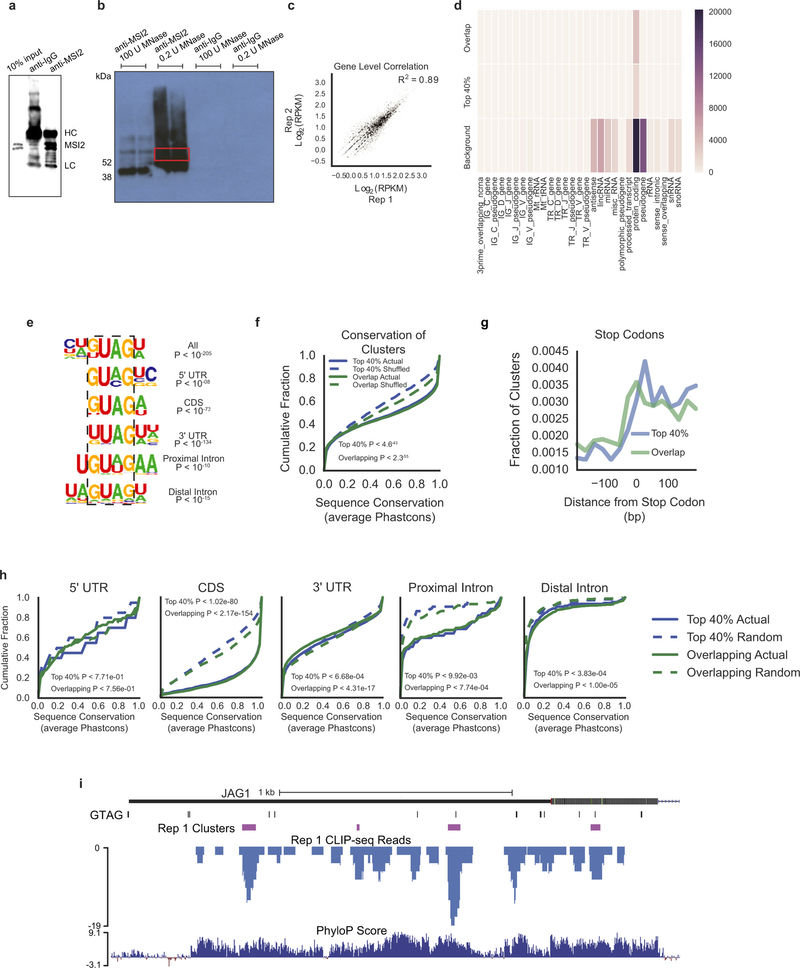
\includegraphics[width=0.5\textwidth]{chapter_4_figures/Figure_S9}
  \caption[Supplementary Figure 3]{. MSI2 preferentially binds mature mRNA within the 3'UTR a, Validation of the capacity of the anti-MSI2 antibody to immunoprecipitate MSI2 compared to IgG control pulldowns. b, Autoradiogram showing anti-MSI2 immunoprecipitated, MNase digested and radiolabelled RNA isolated for CLIP library construction and sequencing (red box). Low levels of MNase show a smearing pattern extending upwards from the modal weight of MSI2. c, Scatter plot of total number of uniquely mapped CLIP-seq reads for each gene, comparing both replicates. d, Heatmap indicating the number of different classes of Gencode annotated genes that contain at least one predicted MSI2 binding site. e, Consensus motifs within MSI2 clusters in the different genic regions. P-values for the most statistically significant enriched motif is presented for all overlapping clusters between replicates. f, Cumulative distribution function of mean conservation score (Phastcons) of MSI2 clusters, compared to a shuffled background control, computed for all overlapping clusters and the top 40\% of overlapping clusters. P- values were obtained by a Kolgomorov-Smirnov two-tailed test comparing the distributions from actual and shuffled locations. g, Number of clusters within 200 bases of the annotated stop codon in known mRNA transcripts for all overlapping clusters between replicates and the top 40\% of overlapping clusters. h, Cumulative distribution function of mean conservation score (Phastcons) of MSI2 clusters, compared to a shuffled background control, computed for overlapping clusters between the replicates and the top 40\% of overlapping clusters found in different genic regions. Similarity in the 3'UTR conservation for the top 40\% with the shuffled background control is likely due to MSI2 sites being small and not needing structural contexts for conservation. P-values were obtained by a Kolgomorov-Smirnov two-tailed test comparing the distributions from actual and shuffled locations. i, Genome browser views displaying CLIP-seq mapped reads from replicate 1 (blue), predicted clusters (purple), exact matches for the GUAG sequence (black) and mammal conservation scores (PhyloP) in the 3' UTRs for a previously predicted Msi1 target. \index{Figure_S3}}
  \label{fig:Figure_S3}
\end{figure}

\begin{figure}[ht]
  \centering
  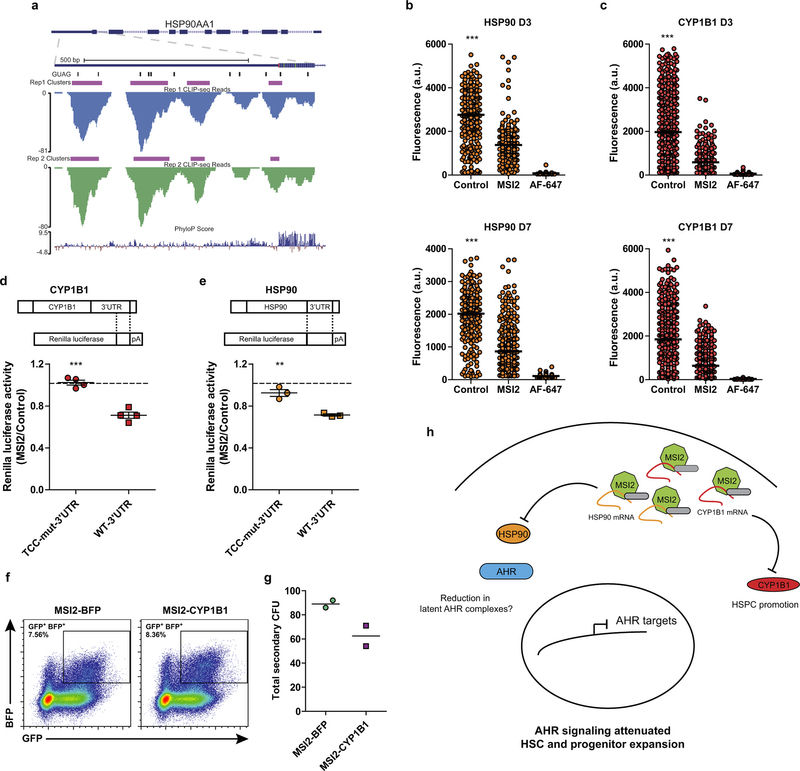
\includegraphics[width=0.5\textwidth]{chapter_4_figures/Figure_S10}
  \caption[Supplementary Figure 4]{. MSI2 OE represses CYP1B1 and HSP90 3'UTR Renilla Luciferase reporter activity a, CLIP-seq reads (replicate 1 in blue and replicate 2 in green) and clusters (purple) mapped to the 3'UTR of HSP90. Matches to the GUAG motif are shown in black. Mammal PhyloP score listed in last track. b and c, Representative data of mean per cell fluoresence for HSP90 and CYP1B1 protein in transduced CD34+ CB. Protein level in cells during in vitro culture was analyzed 3 days (D3) and 7 days (D7) after transduction and sorting for GFP. Corresponding secondary alone antibody staining is shown for each experiment. Each circle represents a cell, and greater than 200 cells were analyzed per condition. d and e, Levels of renilla luciferase activity in NIH-3T3 cells co-transfected with control or MSI2 OE vectors and the CYP1B1 or HSP90 wild type or TCC mutant 3'UTR luciferase reporter (dotted line indicates no change in renilla activity; n=4 CYP1B1 and n=3 HSP90 experiments). f, Flow plots of co-transduced CD34+ CB cells with MSI2 (GFP) and CYP1B1 (BFP) lentivirus. g, GFP+ BFP+ CFU-GEMMs generated from f were replated in to secondary CFU assays and enumerated for total number of colonies formed. A total of 24 CFU-GEMMs from MSI2- BFP and MSI2-CYP1B1 were replated (n=2 experiments). Data presented as mean ± SEM. ***p$<$0.001, **p$<$0.01. h, A model for AHR pathway attenuation through MSI2 post- transcriptional processing. MSI2 mediates the post-transcriptional down regulation of HSP90 at the outset of culture and continuously represses the prominent AHR pathway effector CYP1B1 to facilitate HSPC expansion. The resultant MSI2-mediated repression of AHR signaling enforces a self-renewal program and allows HSPC expansion ex vivo. \index{Figure_S4}}
  \label{fig:Figure_S4}
\end{figure}

\section{METHODS}

\subsection{RIP sample preparation for Western, Northern or RNA-seq analysis}
To monitor protein depletions, if used, and recovery of Flag- or Myc-epitope tagged proteins and/or coprecipitating proteins, a fraction of the input lysate and IP was set aside for Western blotting in 1x SDS loading buffer (60 mM Tris-HCl, pH 6.8, 2\% SDS, 4\% β-mercaptoethanol, 10\% glycerol, 0.1\% bromophenol blue and xylene cyanol). To monitor RNA, Trizol (Ambion) was added to input, unbound, and IP samples. RNA was isolated according to the manufacturer, with 25 μg linear polyacrylamide used as carrier for either library preparation for RNA-seq analysis (see below) or Northern blotting. 

\subsection{RIP-seq and CLIP-seq analysis}
Sequence alignment of CLIP-seq and RIP-seq data to the human genome.
Sequencing reads from CLIP-seq and RIP-seq libraries were first trimmed of polyA tails, adapters, and low quality ends using cutadapt with parameters --match-read-wildcards --times 2 -e 0 -O 5 --quality-cutoff' 6 -m 18 -b TCGTATGCCGTCTTCTGCTTG -b ATCTCGTATGCCGTCTTCTGCTTG -b CGACAGGTTCAGAGTTCTACAGTCCGACGATC -b TGGAATTCTCGGGTGCCAAGG -b AAAAAAAAAAAAAAAAAAAAAAAAAAAAAAAAAAAAAAAAAAAAAAAAAA -b TTTTTTTTTTTTTTTTTTTTTTTTTTTTTTTTTTTTTTTTTTTTTTTTTT. Reads were then mapped against a database of repetitive elements derived from RepBase18.05. Bowtie version 1.0.0 with parameters -S -q -p 16 -e 100 -l 20 was used to align reads against an index generated from Repbase sequences \cite{Langmead2009}. Reads not mapped to Repbase sequences were aligned to the hg19 human genome (UCSC assembly) using STAR \cite{Dobin2013a} version 2.3.0e with parameters --outSAMunmapped Within –outFilterMultimapNmax 1 –outFilterMultimapScoreRange 1.


\subsection{CLIP-seq Cluster Identification and analyses.}
Reads that were PCR replicates were removed from each CLIP-seq library using a custom script. Briefly one read was kept at each nucleotide position when more than one read’s 5' end was mapped. Clusters were then assigned using the CLIPper software with parameters --bonferroni --superlocal --threshold- software \cite{Lovci2013}. Clusters that overlap by at least one base pair are considered overlapping clusters, as determined using bedtools \cite{Quinlan2010} and pybedtools\cite{Dale2011a}.

\subsection{Read Distribution Region Counting and comparisons.}
Genic features were defined using gencode v17 annotations \cite{Harrow2006}. For each gene, all annotated transcripts for that gene were combined and gene level features were generated. 5' UTR, CDS, and 3' UTR regions from gencode genes were identified and merged at the gene level. The number of reads mapping to each annotated meta-region for each gene was counted. Each gene region (3' and 5' UTRs and CDS) was binned into 100 bins, and the mean of reads in each bin was calculated. Then for all genes, the mean of each bin was calculated and plotted. Finally, for each experiment the distribution was normalized to compute a probability density across each bin. To compare different regions, the total number of reads within each region was totaled. For each region the RPK (reads per 1,000 bases) was calculated. To find the percent of reads falling into each region, the percent of RPK normalized reads that were contained within a given region per gene was calculated.

\subsection{Read Distribution Feature Counting.}
For read distributions around specific genic features (termination codons and 3’ transcript ends), features from gencode v17 were selected, the number of reads around each feature was counted, and the mean for each base was calculated across all features. Finally, for each experiment the distribution was normalized to show a probability density across each bin. A background model was generated assuming a uniform distribution of reads distributed to each base, and reads were normally distributed. Each feature at each base is then an independent observation and a z-test was applied to each base (Bonferroni corrected) to see if the reads at that base differed significantly from the background distribution.

\subsection{RIP-seq Analysis.}
RPKMs for each gene annotated in gencode v17 were calculated from RIP-seq data using custom scripts. We determined the fold-change (log2) threshold by which at most 5\% of genes in the FLAG RIP-seq sample were “enriched”. This threshold reflected a false discovery rate (FDR) of 5\%, and was applied to both WT Upf1 and mutant Upf1 RIP-seq samples to identify Upf1 target genes. Non-targets were defined as having a log2 fold change in WT Upf1 RIPs of between -0.05 and 0.05 RPKM

\subsection{UV CLIP–seq library preparation}
CLIP–seq was performed as previously described\cite{Yeo2009}. Briefly, 25 million NB4 cells (a transformed human cell line of haematopoietic origin) were washed in PBS and UV-cross-linked at 400 mJ cm−2 on ice. Cells were pelleted, lysed in wash buffer (PBS, 0.1\% SDS, 0.5\% Na-deoxycholate, 0.5\% NP-40) and DNase-treated, and supernatants from lysates were collected for immunoprecipitation. MSI2 was immunoprecipitated overnight using 5 μg of anti-MSI2 antibody (EP1305Y, Abcam) and Protein A Dynabeads (Invitrogen). Beads containing immunoprecipated RNA were washed twice with wash buffer, high-salt wash buffer (5× PBS, 0.1\% SDS, 0.5\% Na-Deoxycholate, 0.5\% NP-40), and PNK buffer (50 mM Tris-Cl pH 7.4, 10 mM MgCl2, 0.5\% NP-40). Samples were then treated with 0.2 U MNase for 5 min at 37° with shaking to trim immunopreciptated RNA. MNase inactivation was then carried out with PNK + EGTA buffer (50 mM Tris-Cl pH 7.4, 20 mM EGTA, 0.5\% NP-40). The sample was dephosphorylated using alkaline phosphatase (CIP, NEB) at 37° for 10 min followed by washing with PNK+EGTA, PNK buffer, and then 0.1 mg ml−1 BSA in nuclease-free water. 3′RNA linker ligation was performed at 16° overnight with the following adaptor: 5′P-UGGAAUUCUCGGGUGCCAAGG-puromycin. Samples were then washed with PNK buffer, radiolabelled using P32-y-ATP (Perkin Elmer), run on a 4-12\% Bis-Tris gel and then transferred to a nitrocellulose membrane. The nitrocellulose membrane was developed via autoradiography and RNA–protein complexes 15–20 kDa above the molecular weight of MSI2 were extracted with proteinase K followed by RNA extraction with acid phenol-chloroform. A 5′RNA linker (5′HO-GUUCAGAGUUCUACAGUCCGACGAUC-OH) was ligated to the extracted RNA using T4 RNA ligase (Fermentas) for 2 h and the RNA was again purified using acid phenol-chloroform. Adaptor ligated RNA was re-suspended in nuclease-free water and reverse transcribed using Superscript III reverse transcriptase (Invitrogen). Twenty cycles of PCR were performed using NEB Phusion Polymerase using a 3′PCR primer that contained a unique Illumina barcode sequence. PCR products were run on an 8\% TBE gel. Products ranging between 150 and 200 bp were extracted using the QIAquick gel extraction kit (Qiagen) and re-suspended in nuclease-free water. Two separate libraries were prepared and sent for single-end 50-bp Illumina sequencing at the Institute for Genomic Medicine at the University of California, San Diego. 47,098,127 reads from the first library passed quality filtering, of which 73.83\% mapped uniquely to the human genome. 57,970,220 reads from the second library passed quality filtering, of which 69.53\% mapped uniquely to the human genome. CLIP-data reproducibility was verified through high correlation between gene RPKMs and statistically significant overlaps in the clusters and genes within replicates. CLIP–seq data have been deposited in NCBI’s GEO and are accessible through GEO Series accession number GSE69583.


\subsection{CLIP–seq mapping and cluster identification}
Before sequence alignment of CLIP–seq reads to the human genome was performed, sequencing reads from libraries were trimmed of polyA tails, adapters, and low quality ends using Cutadapt with parameters -match-read-wildcards -times 2 -e 0 -O 5 -quality-cutoff 6 -m 18 -b TCGTATGCCGTCTTCTGCTTG -b ATCTCGTATGCCGTCTTCTGCTTG -b CGACAGGTTCAGAGTTCTACAGTCCGACGATC -b TGGAATTCTCGGGTGCCAAGG -b AAAAAAAAAAAAAAAAAAAAAAAAAAAAAAAAAAAAAAAAAAAAAAAAAA -b TTTTTTTTTTTTTTTTTTTTTTTTTTTTTTTTTTTTTTTTTTTTTTTTTT. Reads were then mapped against a database of repetitive elements derived from RepBase (version 18.05). Bowtie (version 1.0.0) with parameters -S -q -p 16 -e 100 -l 20 was used to align reads against an index generated from Repbase sequences\cite{Langmead2009}. Reads not mapped to Repbase sequences were aligned to the hg19 human genome (UCSC assembly) using STAR (version 2.3.0e)\cite{Dobin2013a} with parameters -outSAMunmapped Within -outFilterMultimapNmax 1 -outFilterMultimapScoreRange 1. To identify clusters in the genome of significantly enriched CLIP-seq reads, reads that were PCR replicates were removed from each CLIP–seq library using a custom script of the same method as in \cite{Darnell2012}; otherwise, reads were kept at each nucleotide position when more than one read’s 5′-end was mapped. Clusters were then assigned using the CLIPper software with parameters -bonferroni -superlocal-threshold\cite{Lovci2013}. The ranked list of significant targets was calculated assuming a Poisson distribution, where the observed value is the number of reads in the cluster, and the background is the number of reads across the entire transcript and or across a window of 1000 bp $\pm$ the predicted cluster.

\subsection{Gene annotations for CLIP–seq}
Transcriptomic regions and gene classes were defined using annotations found in gencode v17. Depending on the analysis, clusters were associated by the Gencode-annotated 5′UTR, 3′UTR, CDS or intronic regions. If a cluster overlapped multiple regions, or a single part of a transcript was annotated as multiple regions, clusters were iteratively assigned first as CDS, then 3′UTR, 5′UTR and finally as proximal ($<$500 bases from an exon) or distal ($>$500 bases from an exon) introns. Overlapping peaks were calculated using bedtools and pybedtools\cite{Quinlan2010, Dale2011a}.

\subsection{Gene ontology analysis for CLIP–seq}
Significantly enriched gene ontology (GO) terms were identified using a hypergeometric test that compared the number of genes that were MSI2 targets in each GO term to genes expressed in each GO term as the proper background. Expressed genes were identified using the control samples in SRA study SRP012062. Mapping was performed identically to CLIP–seq mapping, without peak calling and changing the STAR parameter outFilterMultimapNmax to 10. Counts were calculated with featureCounts37 and RPKMs were then computed. Only genes with a mean RPKM $>$ 1 between the two samples were used in the background expressed set.

\subsection{De novo motif and conservation analysis for CLIP–seq}
Randomly located clusters within the same genic regions as predicted MSI2 clusters were used to calculate a background distribution for motif and conservation analyses. Motif analysis was performed using the HOMER algorithm as in \cite{Lovci2013}. For evolutionary sequence conservation analysis, the mean (mammalian) phastCons score for each cluster was used.

%
% Of course, if you prefer, you can just start with
%   \chapter{My First Chapter Name}
% and start typing away.  
\chapter{Just a Test}
This is only a test.
\section{A section}
Lorem ipsum dolor sit amet, consectetuer adipiscing elit. Nulla odio
sem, bibendum ut, aliquam ac, facilisis id, tellus. Nam posuere pede
sit amet ipsum. Etiam dolor. In sodales eros quis pede.  Quisque sed
nulla et ligula vulputate lacinia. In venenatis, ligula id semper
feugiat, ligula odio adipiscing libero, eget mollis nunc erat id orci.
Nullam ante dolor, rutrum eget, vestibulum euismod, pulvinar at, nibh.
In sapien. Quisque ut arcu. Suspendisse potenti. Cras consequat cursus
nulla.

\subsection{A Figure Example}
\label{ssec:figure_example}

This subsection shows a sample figure.

\begin{figure}[ht] 
  \centering
  \includegraphics[width=0.5\textwidth]{sandiego}
  \caption[Short figure caption (must be \protect{$< 4$} lines in the list of figures)]{A picture of San Diego.  Note that figures must be on their own line (no neighboring text) and captions must be single-spaced and appear \protect\textit{below} the figure.  Captions can be as long as you want, but if they are longer than 4 lines in the list of figures, you must provide a short figure caption.\index{SanDiego}} 
  \label{fig:sandiego}
\end{figure}


\subsection{A Table Example}

While in Section \ref{ssec:figure_example} Figure \ref{fig:sandiego} we had a majestic figure, here we provide a crazy table example.

%%%% TABLE 1 %%%%
\vspace{0.25in}
\begin{table}[!ht]
\caption[Short figure caption (must be \protect{$< 4$} lines in the list of tables)]{A table of when I get hungry.  Note that tables must be on their own line (no neighboring text) and captions must be single-spaced and appear \protect\textit{above} the table.  Captions can be as long as you want, but if they are longer than 4 lines in the list of figures, you must provide a short figure caption.}

\vspace{-0.25in}
\begin{center}
\begin{tabular}{|p{1in}|p{2in}|p{3in}|}

\hline
Time of day & Hunger Level & Preferred Food \\

\hline
8am & high & IHOP (French Toast) \\

\hline
noon & medium & Croutons (Tomato Basil Soup \& Granny Smith Chicken Salad) \\

\hline
5pm & high & Bombay Coast (Saag Paneer) or Hi Thai (Pad See Ew) \\

\hline
8pm & medium & Yogurt World (froyo!) \\

\hline
\end{tabular}
\end{center}
\label{tab:analysis3}
\end{table}



%% APPENDIX
\appendix
\chapter{Final notes}
What to do about things \cite{Martin_1983}.  What did he say \cite{Rilling_Insel_1999}.
  Remove me in case of abdominal pain.
  \cite{Arai2006}


%% END MATTER
% \printindex %% Uncomment to display the index
% \nocite{}  %% Put any references that you want to include in the bib 
%               but haven't cited in the braces.
\bibliographystyle{alpha}  %% This is just my personal favorite style. 
%                              There are many others.
%\setlength{\bibleftmargin}{0.25in}  % indent each item
%\setlength{\bibindent}{-\bibleftmargin}  % unindent the first line
%\def\baselinestretch{1.0}  % force single spacing
%\setlength{\bibitemsep}{0.16in}  % add extra space between items
\bibliography{library}  %% This looks for the bibliography in template.bib 
%                          which should be formatted as a bibtex file.
%                          and needs to be separately compiled into a bbl file.
\end{document}

